\documentclass[a4paper,12pt]{report}

\usepackage{geometry}
\geometry{a4paper,left=18mm,right=18mm, top=3cm, bottom=2cm}

\usepackage{lmodern}
\usepackage[T1]{fontenc}
\usepackage{eurosym}
\usepackage{setspace}
\usepackage[latin1]{inputenc}
\usepackage{graphicx}
\usepackage[ngerman]{babel}
\usepackage[solution_on]{mathematik} % solution_on/off
\usepackage{blindtext}
\setcounter{Zufall}{0}


\pagestyle{empty} %PAGESTYLE: empty, plain, fancy
\onehalfspacing %Zeilenabstand
\setcounter{secnumdepth}{-1} % keine Nummerierung der �berschriften



%
%
%%%%%%%%%%%%%%%%%%%%%%%%%%%%%%%%%%%%%%%%%%%%%%%%%%%%%%%%%%%%%%%%%%%%%%%%%%%%%%%%%%%%%%%%%% DOKUMENT - ANFANG %%%%%%%%%%%%%%%%%%%%%%%%%%%%%%%%%%%%%%%%%%%%%%%%%%%%%%%%%%%%%%%%%%%%%%%%%%%%%%%%%%%%%%%
%
%
\begin{document}
\section{02 - MAT - WS 2.3, WS 3.2, WS 3.3 - Aufnahmetest - BIFIE Aufgabensammlung}

\begin{langesbeispiel} \item[0] %PUNKTE DES BEISPIELS
Eine Universität führt für die angemeldeten Bewerber/innen einen Aufnahmetest durch. Dabei werden zehn Multiple-Choice-Fragen gestellt, wobei jede Frage vier Antwortmöglichkeiten hat.
Nur eine davon ist richtig. Wer mindestens acht Fragen richtig beantwortet, wird sicher aufgenommen. Wer alle zehn Fragen richtig beantwortet, erhält zusätzlich ein Leistungsstipendium.
Die Ersteller/innen dieses Tests geben die Wahrscheinlichkeit, bei zufälligem Ankreuzen aller Fragen aufgenommen zu werden, mit 0,04158\,\% an. Nimm an, dass Kandidat $K$ alle
Antworten völlig zufällig ankreuzt.

\subsection{Aufgabenstellung:}

\begin{enumerate}
	\item Nenne zwei Gründe, warum die Anzahl der richtig beantworteten Fragen unter den vorliegenden Angaben binomialverteilt ist! 
	
Gib einen möglichen Grund an, warum in der Realität das Modell der Binomialverteilung hier eigentlich nicht anwendbar ist!
	
	\item Geben Sie die Wahrscheinlichkeit an, dass Kandidat $K$ nicht aufgenommen wird! Berechnen Sie die Wahrscheinlichkeit, dass Kandidat $K$ ein Leistungsstipendium erhält!
\end{enumerate}

\antwort{\subsection{Lösungserwartung:}

\begin{enumerate}
	\item Dieser Aufgabenteil ist durch sinngemäßes Angeben von mindestens zwei der vier angeführten Gründe richtig gelöst: \leer
	
Die Anzahl der richtig beantworteten Fragen ist unter den vorliegenden Angaben binomialverteilt, weil

\begin{itemize}
	\item es nur die beiden Ausgänge "`richtig beantwortet"' und "`falsch beantwortet"' gibt
\item das Experiment unabhängig mit $n = 10$ Mal wiederholt wird
\item die Erfolgswahrscheinlichkeit dabei konstant bleibt
\item es sich dabei um ein "`Bernoulli-Experiment"' handelt
\end{itemize} 

Der zweite Aufgabenteil ist korrekt gelöst, wenn ein Grund (sinngemäß) angeführt wird, z. B.: \leer

\begin{itemize}
	\item Eine Bewerberin/ein Bewerber, die/der sich für ein Studium interessiert, wird sicher
nicht beim Aufnahmetest zufällig ankreuzen.
\item Sobald Kandidat $K$ auch nur eine Antwortmöglichkeit einer Frage ausschließen kann, wäre die Voraussetzung für die Binomialverteilung verletzt. Genau aus diesem Grund
wird die Universität mit zehn Multiple-Choice-Fragen nicht das Auslangen finden, da die Erfolgswahrscheinlichkeit für kompetenzbasiertes Antworten sicher wesentlich höher ist als 0,25.

\item Die Unabhängigkeit der Wiederholung des Zufallsexperiments ist sicher dadurch verletzt, dass die einzelnen Kandidatinnen und Kandidaten aufgrund ihrer Vorbildung
unterschiedliche Erfolgswahrscheinlichkeiten für die Beantwortung der einzelnen Fragen aufweisen. Somit kann unter diesen Voraussetzungen niemals von einer unabhängigen
Wiederholung mit Zählen der Anzahl der Erfolge im Sinne eines Bernoulli-Experiments gesprochen werden.
\end{itemize}

Es sind auch weitere eigenständige Lösungen denkbar. \leer

\item Für die Lösung ist keine Binomialverteilung nötig, da das gesuchte Ereignis das Gegenereignis zur "`Aufnahme"' darstellt. Somit beträgt die (von den Testautorinnen und Testautoren) angegebene Wahrscheinlichkeit:

\[P(\text{Ablehnung})=1-P(\text{Aufnahme})=1-0,0004158=0,9995842\]

Die Ablehnung des Kandidaten $K$ ist somit praktisch sicher.\leer

Auch hier ist keine Binomialverteilung nötig, da ein Zufallsexperiment mit einer Erfolgswahrscheinlichkeit
von 0,25 zehnmal unabhängig wiederholt wird, wobei bei jeder Wiederholung ein "`Erfolg"' eintritt. \leer


Die Wahrscheinlichkeit beträgt somit $P(\text{Leistungsstipendium})=0,25^{10}\approx 0$.
\end{enumerate}
}

				
\end{langesbeispiel}%
\hrule  \leer

\section{3 - MAT - WS 1.1, WS 1.3, WS 3.1, WS 3.2, WS 3.3 - Section Control - BIFIE Aufgabensammlung}

\begin{langesbeispiel} \item[0] %PUNKTE DES BEISPIELS
Der Begriff Section Control (Abschnittskontrolle) bezeichnet ein System zur Überwachung von Tempolimits im Straßenverkehr, bei dem nicht die Geschwindigkeit an einem bestimmten Punkt gemessen wird, sondern die Durchschnittsgeschwindigkeit über eine längere Strecke. Dies geschieht mithilfe von zwei Überkopfkontrollpunkten, die mit Kameras ausgestattet sind. 
Das Fahrzeug wird sowohl beim ersten als auch beim zweiten Kontrollpunkt fotografiert.
 
Die zulässige Höchstgeschwindigkeit bei einer bestimmten Abschnittskontrolle beträgt $100\,$km/h. Da die Polizei eine Toleranz kleiner $3\,$km/h gewährt, löst die Section Control bei $103\,$km/h aus. Lenker/innen von Fahrzeugen, die dieses Limit erreichen oder überschreiten, machen sich strafbar und werden im Folgenden als "`Temposünder"' bezeichnet.

Eine Stichprobe der Durchschnittsgeschwindigkeiten von zehn Fahrzeugen ist in der nachfolgenden Tabelle aufgelistet und im abgebildeten Boxplot dargestellt.
				\leer
				
				\begin{tabular}{|c|c|c|c|c|c|c|c|c|c|c|} \hline
				$v$ in $km/h$&88&113&93&98&121&98&90&98&105&129 \\ \hline				
				\end{tabular}
				\leer
				
				\begin{center}\newrgbcolor{zzttqq}{0.6 0.2 0.}
\psset{xunit=0.3cm,yunit=0.3cm,algebraic=true,dimen=middle,dotstyle=o,dotsize=5pt 0,linewidth=0.8pt,arrowsize=3pt 2,arrowinset=0.25}
\begin{pspicture*}(84.8,-2.)(131.,7.765)
\multips(86,0)(1.0,0){45}{\psline[linestyle=dashed,linecap=1,dash=1.5pt 1.5pt,linewidth=0.4pt,linecolor=gray]{c-c}(0,0)(0,7.765)}
\psaxes[labelFontSize=\scriptstyle,xAxis=true,yAxis=true,Dx=2.,Dy=5.,ticksize=-2pt 0,subticks=2]{->}(0,0)(86.08,-2.)(131.,7.765)
\psframe[linecolor=zzttqq,fillcolor=zzttqq,fillstyle=solid,opacity=0.1](93.,1.0)(113.,5.)
\psline[linecolor=zzttqq,fillcolor=zzttqq,fillstyle=solid,opacity=0.1](88.,1.)(88.,5.)
\psline[linecolor=zzttqq,fillcolor=zzttqq,fillstyle=solid,opacity=0.1](129.,1.)(129.,5.)
\psline[linecolor=zzttqq,fillcolor=zzttqq,fillstyle=solid,opacity=0.1](98.,1.)(98.,5.)
\psline[linecolor=zzttqq,fillcolor=zzttqq,fillstyle=solid,opacity=0.1](88.,3.)(93.,3.)
\psline[linecolor=zzttqq,fillcolor=zzttqq,fillstyle=solid,opacity=0.1](113.,3.)(129.,3.)
\end{pspicture*}\end{center}%Aufgabentext

\begin{aufgabenstellung}
\item %Aufgabentext

\Subitem{Bestimme den arithmetischen Mittelwert $\overline{x}$ und die empirische Standardabweichung $s$ der Durchschnittsgeschwindigkeiten in der Stichprobe!} %Unterpunkt1
\Subitem{Kreuze die zutreffende(n) Aussage(n) zur Standardabweichung an!

\multiplechoice[5]{  %Anzahl der Antwortmoeglichkeiten, Standard: 5
					L1={Die Standardabweichung ist ein Maß für die Streuung um den arithmetischen Mittelwert.},   %1. Antwortmoeglichkeit 
					L2={Die Standardabweichung ist immer ca. ein Zehntel des arithmetischen Mittelwerts.},   %2. Antwortmoeglichkeit
					L3={Die Varianz ist die quadrierte Standardabweichung.},   %3. Antwortmoeglichkeit
					L4={Im Intervall $[\overline{x}-s;\overline{x}+2]$ der obigen Stichprobe liegen ca. $60\,\%$ bis $80\,\%$ der Werte.},   %4. Antwortmoeglichkeit
					L5={Die Standardabweichung ist der arithmetische Mittelwert der Abweichung von 	$\overline{x}$.},	 %5. Antwortmoeglichkeit
					L6={},	 %6. Antwortmoeglichkeit
					L7={},	 %7. Antwortmoeglichkeit
					L8={},	 %8. Antwortmoeglichkeit
					L9={},	 %9. Antwortmoeglichkeit
					%% LOESUNG: %%
					A1=1,  % 1. Antwort
					A2=3,	 % 2. Antwort
					A3=4,  % 3. Antwort
					A4=0,  % 4. Antwort
					A5=0,  % 5. Antwort
					}} %Unterpunkt2

\item %Aufgabentext

\Subitem{Bestimme aus dem Boxplot (Kastenschaubild) der Stichprobe den Median sowie das obere und untere Quartil.} %Unterpunkt1
\Subitem{Gib an, welche zwei Streumaße aus dem Boxplot ablesbar sind. Bestimme auch deren Werte.} %Unterpunkt2

\item Die Erfahrung zeigt, dass die Wahrscheinlichkeit, ein zufällig ausgewähltes Fahrzeug mit einer Durchschnittsgeschwindigkeit von mindestens $103\,km/h$ zu erfassen, $14\,\%$ beträgt. %Aufgabentext

\Subitem{Berechne den Erwartungswert $\mu$ und die Standardabweichung $\sigma$ der Temposünder unter fünfzig zufällig ausgewählten Fahrzeuglenkern.} %Unterpunkt1
\Subitem{Berechne, wie groß die Wahrscheinlichkeit ist, dass die Anzahl der Temposünder unter fünfzig Fahrzeuglenkern innerhalb der einfachen Standardabweichung um den Erwartungswert, d.h. im Intervall $[\mu-\sigma;\mu+\sigma]$ liegt.} %Unterpunkt2

\end{aufgabenstellung}

\begin{loesung}
\item \subsection{Lösungserwartung:} 

\Subitem{$\overline{x}=\frac{1}{10}\cdot\sum_{i=1}^{10}{x_i=103,3}\,km/h$

$s=\sqrt{\frac{1}{9}\cdot\sum_{i=1}^{10}{(x_i-\overline{x})^2}}=13,6\,km/h$} %Lösung von Unterpunkt1
\Subitem{Richtige MC-Antworten: 1,3,4} %%Lösung von Unterpunkt2

\setcounter{subitemcounter}{0}
\subsection{Lösungsschlüssel:}
 
\Subitem{Ein Punkt für die richtige Berechnung des arithmetischen Mittelwerts und der Standardabweichung.} %Lösungschlüssel von Unterpunkt1
\Subitem{Ein Punkt für die korrekten Antworten.} %Lösungschlüssel von Unterpunkt2

\item \subsection{Lösungserwartung:} 

\Subitem{Median ... $98\,$km/h\qquad unteres Quartil ... $93\,$km/h\qquad oberes Quartil ... $113\,$km/h} %Lösung von Unterpunkt1
\Subitem{Spannweite ... $41\,$km/h\qquad Quartilsabstand ... $20\,$km/h} %%Lösung von Unterpunkt2

\setcounter{subitemcounter}{0}
\subsection{Lösungsschlüssel:}
 
\Subitem{Ein Punkt für die korrekten Werte.} %Lösungschlüssel von Unterpunkt1
\Subitem{Ein Punkt für die korrekten Werte.} %Lösungschlüssel von Unterpunkt2

\item \subsection{Lösungserwartung:} 

\Subitem{$\mu=n\cdot p=50\cdot 0,14=7$\qquad $\sigma=\sqrt{\mu\cdot (1-p)}=2,45$} %Lösung von Unterpunkt1
\Subitem{$P(\mu-\sigma<X<\mu+\sigma)=P(5\leq X\leq 9)=P(X=5)+P(X=6)+P(X=7)+P(X=8)+P(X=9)=0,1286+0,1570+0,1606+0,1406+0,1068=0,6936=69,36\,\%$} %%Lösung von Unterpunkt2

\setcounter{subitemcounter}{0}
\subsection{Lösungsschlüssel:}
 
\Subitem{Ein Punkt für die korrekten Werte.} %Lösungschlüssel von Unterpunkt1
\Subitem{Ein Punkt für die korrekte Wahrscheinlichkeit.} %Lösungschlüssel von Unterpunkt2

\end{loesung}

\end{langesbeispiel}%
\hrule  \leer

\section{5 - MAT - WS 2.2, WS 3.1, WS 3.3 - Mathematikschularbeiten - BIFIE Aufgabensammlung}

\begin{langesbeispiel} \item[0] %PUNKTE DES BEISPIELS
Wenn in der Oberstufe in einem Semester höchstens zwei Mathematikschularbeiten vorgesehen sind, muss jede versäumte Schularbeit nachgeholt werden.
				Ein Mathematiklehrer hat auf Basis seiner langjährigen Erfahrung die untenstehende Tabelle erstellt. Dabei beschreibt $h(n)$ die relative Häufigkeit, dass bei einer Schularbeit insgesamt $n$ Schüler/innen fehlen.\vspace{0,3cm}
				
\begin{center}
				\begin{tabular}{|c|c|c|c|c|c|c|c|c|c|} \hline
				$n$&0&1&2&3&4&5&6&7&>7\\ \hline
				$h(n)$&0,15&0,15&0,2&0,3&0,1&0,05&0,03&0,02&0\\ \hline
				\end{tabular}	
\end{center}%Aufgabentext

\begin{aufgabenstellung}
\item %Aufgabentext

\Subitem{Gib an, mit wie vielen Fehlenden der Mathematiklehrer im Durchschnitt bei jeder Schularbeit rechnen muss.} %Unterpunkt1
\Subitem{Lässt sich aus dem errechneten Durchschnittswert mit Sicherheit behaupten, dass bei jeder Mathematikschularbeit mindestens eine Schülerin/ein Schüler fehlt? Begründe deine Antwort.} %Unterpunkt2

\item %Aufgabentext

\Subitem{Kreuze die beiden zutreffenden Aussagen an!
	
	\multiplechoice[5]{  %Anzahl der Antwortmoeglichkeiten, Standard: 5
					L1={Es kann nie passieren, dass acht Schüler/innen bei einer Schularbeit fehlen.},   %1. Antwortmoeglichkeit 
					L2={Die Wahrscheinlichkeit, dass bei einer Mathematikschularbeit niemand fehlt, ist gleich groß wie die Wahrscheinlichkeit, dass eine Schülerin/ein Schüler fehlt.},   %2. Antwortmoeglichkeit
					L3={Die Wahrscheinlichkeit, dass drei Schüler/innen bei einer Mathematikschularbeit fehlen, ist größer als die Wahrscheinlichkeit, dass höchstens zwei oder mindestens vier Schüler/innen fehlen.},   %3. Antwortmoeglichkeit
					L4={Die Wahrscheinlichkeit, dass eine Schularbeit nachgeholt werden muss, weil mindestens eine Schülerin/ein Schüler fehlt, beträgt $85\,\%$.},   %4. Antwortmoeglichkeit
					L5={Im Durchschnitt muss eine von vier Schularbeiten pro Jahr nicht nachgeholt werden.},	 %5. Antwortmoeglichkeit
					L6={},	 %6. Antwortmoeglichkeit
					L7={},	 %7. Antwortmoeglichkeit
					L8={},	 %8. Antwortmoeglichkeit
					L9={},	 %9. Antwortmoeglichkeit
					%% LOESUNG: %%
					A1=2,  % 1. Antwort
					A2=4,	 % 2. Antwort
					A3=0,  % 3. Antwort
					A4=0,  % 4. Antwort
					A5=0,  % 5. Antwort
					}} %Unterpunkt1
					
In einer bestimmten Klasse werden im kommenden Schuljahr vier Schularbeiten (zwei pro Semester) geschrieben.

\Subitem{Gib einen Term an, mit dem die Wahrscheinlichkeitsverteilung für die Anzahl der Mathematikschularbeiten dieser Klasse, die aufgrund fehlender SchülerInnen nachgeholt werden müssen, berechnet werden kann!
					
					$P(X=k)=$ \antwort[\rule{3cm}{0.3pt}]{$\Vek{4}{k}{}\cdot 0,85^k\cdot 0,15^{4-k}$} mit $k=$ \antwort[\rule{3cm}{0.3pt}]{0,1,2,...,4}} %Unterpunkt2

\end{aufgabenstellung}

\begin{loesung}
\item \subsection{Lösungserwartung:} 

\Subitem{Im Durchschnitt muss der Mathematiklehrer mit 2,42 Fehlenden rechnen.} %Lösung von Unterpunkt1
\Subitem{Daraus lässt sich nicht mit Sicherheit behaupten, dass bei jeder Mathematikschularbeit jemand fehlt, da es sich dabei um eine statistische Kenngröße handelt, die keine konkrete Aussage über die einzelne Schularbeit erlaubt.} %%Lösung von Unterpunkt2

\setcounter{subitemcounter}{0}
\subsection{Lösungsschlüssel:}
 
\Subitem{Ein Punkt für die korrekte Angabe der zu erwartenden Anzahl. Eine auf ganze Zahlen gerundete Antwort ist nicht korrekt, da der Erwartungswert nur statistische Aussagekraft hat und somit die Rundung die Aussage verändert.} %Lösungschlüssel von Unterpunkt1
\Subitem{Ein Punkt für eine korrekte Begründung. Eine Schülerantwort, die darauf abzielt, dass es entsprechend der empirischen Häufigkeitsverteilung mit $15\,\%$iger Häufigkeit zu keinem Fehlen kommt, ist als nicht korrekt zu bewerten, da in der Aufgabenstellung verlangt wird, den Erwartungswert zu interpretieren.} %Lösungschlüssel von Unterpunkt2

\item \subsection{Lösungserwartung:} 

\Subitem{Richtigen MC-Antworten: 2,4} %Lösung von Unterpunkt1
\Subitem{$P(X=k)=\Vek{4}{k}{}\cdot 0,85^k\cdot 0,15^{4-k}$ mit $k=0,1,2,...,4$} %%Lösung von Unterpunkt2

\setcounter{subitemcounter}{0}
\subsection{Lösungsschlüssel:}
 
\Subitem{Ein Punkt für die richtigen MC-Antworten.} %Lösungschlüssel von Unterpunkt1
\Subitem{Ein Punkt für den richtigen Term.} %Lösungschlüssel von Unterpunkt2

\end{loesung}

\end{langesbeispiel}%
\hrule  \leer

\section{6 - MAT - WS 2.2, WS 3.1, WS 3.2 - Ärztliche Untersuchung an einer Schule - BIFIE Aufgabensammlung}

\begin{langesbeispiel} \item[0] %PUNKTE DES BEISPIELS
Eine Schulärztin hat die Untersuchung der Oberstufenschüler/innen einer Schule abgeschlossen. Die Auswertung der Ergebnisse ist in den nachstehenden Abbildungen grafisch dargestellt.
				\leer
				\begin{center}
				\begin{tabular}{|c|c|} \hline
				Mädchen&Burschen\\ \hline
				\multicolumn{2}{|c|}{Körpergröße}\\
				\multicolumn{1}{|c}{\resizebox{0.3\linewidth}{!}{\kreisdiagramm\begin{tikzpicture}
				\tikzstyle{every node}=[font=\footnotesize]
				\pie[color={black!10 ,black!20 , black!30, black!40}, %Farbe
				text=inside %Format: inside,pin, legend
				]
				{22/unter 150\,cm , 14/über 175\,cm , 64/150-175\,cm} %Werte
				\end{tikzpicture}}}&\multicolumn{1}{c|}{\resizebox{0.3\linewidth}{!}{\kreisdiagramm\begin{tikzpicture}
				\tikzstyle{every node}=[font=\footnotesize]
				\pie[color={black!10 ,black!20 , black!30, black!40}, %Farbe
				text=inside %Format: inside,pin, legend
				]
				{7/unter 150\,cm , 34/über 175\,cm , 59/150-175\,cm} %Werte
				\end{tikzpicture}}}\\ \hline
				\multicolumn{2}{|c|}{Gewicht}\\
				\multicolumn{1}{|c}{\resizebox{0.3\linewidth}{!}{\kreisdiagramm\begin{tikzpicture}
				\tikzstyle{every node}=[font=\footnotesize]
				\pie[color={black!10 ,black!20 , black!30, black!40}, %Farbe
				text=inside %Format: inside,pin, legend
				]
				{28/Untergewicht , 11/Übergewicht, 61/Normalgewicht} %Werte
				\end{tikzpicture}}}&\multicolumn{1}{c|}{\resizebox{0.3\linewidth}{!}{\kreisdiagramm\begin{tikzpicture}
				\tikzstyle{every node}=[font=\footnotesize]
				\pie[color={black!10 ,black!20 , black!30, black!40}, %Farbe
				text=inside %Format: inside,pin, legend
				]
				{13/Untergewicht, 21/Übergewicht, 66/Normalgewicht} %Werte
				\end{tikzpicture}}}\\ \hline
				\multicolumn{2}{|c|}{Rauchverhalten}\\
				\multicolumn{1}{|c}{\resizebox{0.3\linewidth}{!}{\kreisdiagramm\begin{tikzpicture}
				\tikzstyle{every node}=[font=\footnotesize]
				\pie[color={black!10 ,black!20 , black!30, black!40}, %Farbe
				text=inside %Format: inside,pin, legend
				]
				{42/Raucherinnen, 58/Nichtraucherinnen} %Werte
				\end{tikzpicture}}}&\multicolumn{1}{c|}{\resizebox{0.3\linewidth}{!}{\kreisdiagramm\begin{tikzpicture}
				\tikzstyle{every node}=[font=\footnotesize]
				\pie[color={black!10 ,black!20 , black!30, black!40}, %Farbe
				text=inside %Format: inside,pin, legend
				]
				{37/Raucher, 63/Nichtraucher} %Werte
				\end{tikzpicture}}}\\ \hline
				\end{tabular}
				\end{center}
				
Von den einzelnen Klassen wurde dabei folgende Schüleranzahl erfasst:
				
				\begin{center}
				\begin{tabular}{|c||c|c|c|c|c|c|c|c|}\hline
				Klasse&5A&5B&6A&6B&7A&7B&8A&8B\\ \hline \hline
				weiblich&18&22&20&16&16&15&12&18\\ \hline
				männlich&14&9&7&9&10&11&13&8\\ \hline \hline
				gesamt&32&31&27&25&26&26&25&26\\ \hline
				\end{tabular}
				\end{center}%Aufgabentext

\begin{aufgabenstellung}
\item %Aufgabentext

\Subitem{Gib auf Basis der erhobenen Daten einen Term zur Berechnung der Wahrscheinlichkeit für folgendes Ereignis an, wobei angenommen wird, dass die angegebenen Prozentsätze unabhängig von der Schulstufe sind: 
\begin{center}
"`In den 5. Klassen gibt es höchstens 2 Raucherinnen."'
\end{center}} %Unterpunkt1

In dieser Schule wurden die Schüler/innen nicht nach Klassen geordnet untersucht, sondern jede/r entschied selbst, wann sie/er zur Schulärztin ging (zufällige Reihenfolge angenommen).

\Subitem{Wie viele Schüler/innen musste die Schulärztin untersuchen, um mit absoluter Sicherheit mindestens eine Raucherin/einen Raucher aus den 5. Klassen zu finden, wenn sie weiß, dass es in den 5. Klassen mindestens eine/n davon gibt?} %Unterpunkt2

\item Auf Basis der oben angeführten Daten wurde für die Burschen eines Jahrgangs der folgende statistische Kennwert ermittelt:
\begin{center}
$\mu=n\cdot p=23\cdot 0,34=7,82$
\end{center} %Aufgabentext

\Subitem{Was drückt dieser Kennwert aus? Interpretiere diesen Kennwert im gegebenen 
Zusammenhang und nutzen Sie dabei sowohl die grafische Abbildung der Untersuchungsergebnisse als auch die tabellarische Übersicht über die Klassenschülerzahlen.} %Unterpunkt1
\Subitem{Ist der so errechnete Kennwert aussagekräftig? Begründe deine Antwort.} %Unterpunkt2

\end{aufgabenstellung}

\begin{loesung}
\item \subsection{Lösungserwartung:} 

\Subitem{$X$ ... Anzahl der Raucherinnen aus allen 5. Klassen
	
	$X$ ... Binomialverteilung mit $n=40,p=0,42$
	
	$P(X\leq2)=P(X=0)+P(X=1)+P(X=2)=$
	
	$=\binom{40}{0}\cdot 0,42^0\cdot 0,58^{40}+\binom{40}{1}\cdot 0,42^1\cdot 0,58^{39}+\binom{40}{2}\cdot 0,42^2\cdot 0,58^{38}$} %Lösung von Unterpunkt1
\Subitem{Da in der Angabe nur statistische Aussagen gemacht werden, aufgrund derer nicht mit Sicherheit behauptet werden kann, ob es mehr als eine Raucherin/einen Raucher in den 5. Klassen gibt, müssen alle Schüler/innen untersucht werden, um mit Sicherheit eine Raucherin/einen Raucher in der 5. Klasse zu finden.} %%Lösung von Unterpunkt2

\setcounter{subitemcounter}{0}
\subsection{Lösungsschlüssel:}
 
\Subitem{Ein Punkt für einen korrekten Term.} %Lösungschlüssel von Unterpunkt1
\Subitem{Ein Punkt für die richtige Angabe der zu untersuchenden Schüler/innen.} %Lösungschlüssel von Unterpunkt2

\item \subsection{Lösungserwartung:} 

\Subitem{In allen 5. Klassen zusammen gibt es 23 Burschen. Der Prozentsatz der Burschen mit einer Körpergröße von über 175 cm beträgt 34\,\%.
	
Somit drückt der berechnete Wert $\mu=n\cdot p=23\cdot 0,34=7,82$ die Anzahl der zu erwartenden Burschen in den 5. Klassen mit einer Körpergröße von über 175 cm aus.} %Lösung von Unterpunkt1
\Subitem{Da die Daten für die gesamte Oberstufe ausgewertet sind und Schüler/innen während der Oberstufe noch wachsen, werden voraussichtlich weniger so große Schüler in den 5. Klassen zu finden sein. Somit ist der errechnete Erwartungswert nicht aussagekräftig bzw. sinnvoll.} %%Lösung von Unterpunkt2

\setcounter{subitemcounter}{0}
\subsection{Lösungsschlüssel:}
 
\Subitem{Ein Punkt für die korrekte Deutung des Kennwerts.

Wesentlich für die Richtigkeit der Antwort sind:
\subitem $\circ$ sinngemäße Formulierung für "`Erwartungswert"'
\subitem $\circ$ Burschen aus 5. Klassen mit über 175 cm Körpergröße 

Eine Rundung auf 8 ist in diesem Zusammenhang als falsch zu werten, da
 es sich bei $\mu$ nur um einen statistischen Kennwert und nicht um einen realen Ausgang eines Zufallsexperiments handelt.} %Lösungschlüssel von Unterpunkt1
\Subitem{Ein Punkt für eine korrekte Begründung.

Wesentlich für die Richtigkeit der Antwort ist die sinngemäße Darstellung einer der folgenden Interpretationen:
\subitem $\circ$ Die unabhängige Wiederholung (im Sinne des Bernoulli-Experiments) ist nicht gegeben.
\subitem $\circ$ Die verwendete Wahrscheinlichkeit (über 175 cm Körpergröße) bzw. relative Häufigkeit ist auf die beobachtete Eigenschaft (Bursch aus 5. Klassen) nicht anzuwenden.

Die Burschen/Jugendlichen wachsen im Laufe der Oberstufe, daher ist die relative Häufigkeit auf diese Gruppe nur eingeschränkt übertragbar.} %Lösungschlüssel von Unterpunkt2

\end{loesung}

\end{langesbeispiel}%
\hrule  \leer

\section{07 - MAT - FA 1.4, WS 3.1 - Glücksrad - BIFIE Aufgabensammlung}

\begin{langesbeispiel} \item[0] %PUNKTE DES BEISPIELS
				Auf einem Jahrmarkt werden nach dem Drehen eines Glücksrades \EUR{0}, \EUR{1}, \EUR{2} oder \EUR{4} ausbezahlt.Jedes Mal, bevor das Rad gedreht wird, ist eine Spielgebühr $e$ (in \euro) zu entrichten.
				
Der Spielbetreiber hat für mathematisch Interessierte den Graphen einer sogenannten kumulativen Verteilungsfunktion $F$ mit $F(x)=P(X \leq x)$ angegeben. Die Zufallsvariable $X$ gibt dabei die Größe des auszuzahlenden Betrags an. Aus der Abbildung lassen sich die Wahrscheinlichkeiten für die einzelnen Auszahlungsbeträge ermitteln, wobei die Variable $x$ angibt, welche Werte die Zufallsvariable $X$ annimmt, d.h. wie groß die einzelnen auszuzahlenden Beträge sind.

Bei diesem Spiel sind sie, wie oben angegeben, \EUR{0}, \EUR{1}, \EUR{2} oder \EUR{4}. 
				\leer
				\begin{center}
				\resizebox{0.8\linewidth}{!}{\psset{xunit=2cm,yunit=10cm,algebraic=true,dimen=middle,dotstyle=o,dotsize=5pt 0,linewidth=0.8pt,arrowsize=3pt 2,arrowinset=0.25}
\begin{pspicture*}(-0.7907949790794977,-0.15)(5.2,1.0757839248873753)
\psaxes[labelFontSize=\scriptstyle,xAxis=true,yAxis=true,Dx=1.,Dy=0.1,ticksize=-2pt 0,subticks=2]{->}(0,0)(-0.7907949790794977,-0.15)(5.2,1.0757839248873753)[x,140] [y,-40]
\psline[linewidth=2.pt](0.,0.2)(1.,0.2)
\psline[linewidth=2.pt](1.,0.5)(2.,0.5)
\psline[linewidth=2.pt](2.,0.9)(4.,0.9)
\psline[linewidth=2.pt](4.,1.)(6.,1.)
\psline[linewidth=2.pt](0.,0.)(-2.,0.)
\begin{scriptsize}
\psdots[dotstyle=*](0.,0.2)
\psdots(1.,0.2)
\psdots[dotstyle=*](1.,0.5)
\psdots(2.,0.5)
\psdots[dotstyle=*](2.,0.9)
\psdots(4.,0.9)
\psdots[dotstyle=*](4.,1.)
\psdots(6.,1.)
\psdots(0.,0.)
\psdots[dotstyle=*,linecolor=blue](-2.,0.)
\end{scriptsize}
\end{pspicture*}}
				\end{center}
				
\subsection{Aufgabenstellung:}
\begin{enumerate}
	\item Ermittle mithilfe der Graphik die Wahrscheinlichkeitsverteilung der Zufallsvariablen $X$ und trag die entsprechenden Werte in der nachstehenden Tabelle ein!
	\leer
	
	\begin{tabular}{|l|C{2cm}|C{2cm}|C{2cm}|C{2cm}|}\hline
	Ausbezahlungsbetrag $x$ in \euro&0&1&2&4\\ \hline
	P(X=x) &\antwort{0,2}&\antwort{0,3}&\antwort{0,4}&\antwort{0,1}\\ \hline
	\end{tabular}

Begründe, warum die Funktion $F$ monoton steigend ist und warum das Maximum von $F$ immer 1 sein muss!

\item Der Erwartungswert von $X$ beträgt bei diesem Spiel \EUR{1,50}, d. h., im Mittel beträgt der auszuzahlende Betrag \EUR{1,50}.

Versetze dich in die Lage des Spielbetreibers. Wie groß wählst du den Betrag der Spielgebühr $e$ pro Drehung mindestens, wenn du die Größe des Erwartungswerts von $X$ kennst? Gib eine Begründung für deine Wahl an!

Die Zufallsvariable $Y$ gibt die Höhe des (tatsächlichen) Gewinns aus der Sicht 
der Spielerin/des Spielers an. 

Welche Werte $y$ wird der Gewinn in Abhängigkeit von $e$ bei den bekannten Auszahlungsbeträgen \EUR{0}, \EUR{1}, \EUR{2} oder \EUR{4} annehmen?
 
Vervollständige die Tabelle und gib die Wahrscheinlichkeitsverteilung von 
$Y$ an!
\leer

\begin{tabular}{|l|C{2cm}|C{2cm}|C{2cm}|C{2cm}|}\hline
	Gewinn $y$ in \euro&\antwort{$0-e$}&\antwort{$1-e$}&\antwort{$2-e$}&\antwort{$4-e$} \\ \hline
	$P(Y=y)$ &\antwort{0,2}&\antwort{0,3}&\antwort{0,4}&\antwort{0,1}\\ \hline
	\end{tabular}
\end{enumerate}
	
\antwort{\subsection{Lösungserwartung:}
\begin{enumerate}
	\item Tabelle: siehe oben!
	
	Eine kumulierte Verteilungsfunktion entsteht durch Summenbildung der Einzelwahrscheinlichkeiten. Da die Einzelwahrscheinlichkeiten definitionsgemäß immer größer oder gleich 0 sein müssen, ist die Funktion $F$ monoton steigend. Das Maximum muss 1 sein, da die Summe aller Einzelwahrscheinlichkeiten einer Wahrscheinlichkeitsverteilung 1 ergeben muss.
	
	\item Tabelle: siehe oben!
	
	$e$ muss größer als \EUR{1,50} sein, da der Spielbetreiber auf lange Sicht einen Gewinn und keinen Verlust erzielen möchte, der sich aus $e-1,5>0$ errechnet.
\end{enumerate}}
\end{langesbeispiel}%
\hrule  \leer

\section{14 - MAT - AG 2.2, FA 1.7, FA 5.2, WS 2.3, WS 3.1, WS 3.3 - Schwarzfahren als Volkssport - BIFIE Aufgabensammlung}

\begin{langesbeispiel} \item[0] %PUNKTE DES BEISPIELS
				Im Jahr 2010 wurden in den Graz-Linien exakt 36\,449 Schwarzfahrer und Schwarzfahrerinnen auf frischer Tat ertappt.  
				
\textit{"`Ihren Fahrschein, bitte!"' - diese freundliche, aber bestimmte Aufforderung treibt Schwarzfahrern regelm��ig den Angstschwei� ins Gesicht. Zu Recht, hei�t es dann doch 65 Euro Strafe zahlen. Mehr als 800\,000 Fahrschein-
kontrollen wurden im Vorjahr in den Grazer Bus- und Stra�enbahnlinien durchgef�hrt. 36\,449 Personen waren Schwarzfahrer. Gegen�ber 2009 ist das ein leichtes Minus von 300 Beanstandungen. F�r die Graz-Linien ist das ein Beweis f�r den Erfolg der strengen Kontrollen. F�r den Vorstand der Graz-Linien steht darum eines fest: "`Wir werden im Interesse unserer zahlenden Fahrg�ste 
auch 2011 die Kontrollen im gleichen Ausma� fortsetzen."' Denn den Graz-Linien entgehen durch den Volkssport Schwarzfahren jedes Jahr Millionen. Rechnet m
an die Quote der bei den Kontrollen ertappten Schwarzfahrer (ca. 5\,\%) 
auf die Gesamtzahl der bef�rderten Personen hoch (ca. 100 Mio. pro Jahr), dann werden aus 36\,449 schnell f�nf Millionen, die aufs Ticket pfeifen...} 

\begin{footnotesize}(Quelle: Meine Woche Graz, April 2011, adaptiert)\end{footnotesize}

In diesem Zeitungsartikel wird der Begriff Schwarzfahrer f�r Personen, die ohne g�ltigen Fahrschein angetroffen werden, verwendet. Fahrg�ste, die ihre Zeitkarte (z. B. Wochenkarte, Sch�lerfreifahrtsausweis) nicht bei sich haben,
 gelten nicht als Schwarzfahrer/innen. 

Nach Angaben der Graz-Linien betr�gt der Anteil der Schwarzfahrer/innen etwa 5\,\%. 

Zwei Kontrolleure steigen an der Haltestelle Jakominiplatz in einen Wagen der Stra�enbahnlinie 5 und kontrollieren alle 25 Fahrg�ste. An der Haltestelle 
Hauptplatz steigen sie in einen Wagen der Linie 3 um, in dem sie alle 18 Fahrg�ste kontrollieren.
				
\subsection{Aufgabenstellung:}
\begin{enumerate}
	\item Es soll die Wahrscheinlichkeit $p_1$ berechnet werden, dass die Kontrolleure mindestens eine Schwarzfahrerin/einen Schwarzfahrer ermitteln, aber erst in der Linie 3 auf diese Person treffen. Gib einen geeigneten Term an, mit dem diese Wahrscheinlichkeit $p_1$ ermittelt werden kann, und berechne diese! 
	
Es sei $p_2$ die Wahrscheinlichkeit, bereits im Wagen der Linie 5 auf mindestens eine Schwarzfahrerin/einen Schwarzfahrer zu treffen. Begr�nde, warum $p_2$ gr��er als $p_1$ sein muss, ohne $p_2$ zu berechnen!

\item  Es wird angenommen, dass bei den durchgef�hrten Kontrollen nur 1\,\% aller f�nf Millionen Personen, die keinen Fahrschein mithaben, entdeckt werden. Man wei�, dass 10\,\% dieser f�nf Millionen Personen eine Zeitkarte besitzen, die sie aber nicht bei sich haben, und daher nicht als Schwarzfahrer/innen gelten. Wird eine Schwarzfahrerin/ein Schwarzfahrer erwischt, muss sie/er zus�tzlich zum Fahrpreis von \EUR{2} noch \EUR{65} Strafe zahlen. Gehe 
davon aus, dass im Durchschnitt die nicht erwischten Schwarzfahrer/innen jeweils entgangene Einnahmen eines Einzelfahrscheins von \EUR{2} verursachen.
  
Berechne den in einem Jahr durch die Schwarzfahrer/innen entstandenen finanziellen Verlust f�r die Grazer Linien! 

Das Bu�geld m�sste wesentlich erh�ht werden, um eine Kostendeckung zu erreichen. Ermittle den neuen Betrag f�r ein kostendeckendes Bu�geld!

\item Die Anzahl der entdeckten Schwarzfahrer/innen nahm gegen�ber 2009 um 300 ab und betrug 2010 nur mehr 36\,449. Man geht davon aus, dass durch verst�rkte Kontrollen eine weitere Abnahme der Anzahl an Schwarzfahrerinnen/Schwarzfahrern erreicht werden kann. 

Beschreibe diese Abnahme beginnend mit dem Jahr 2009 sowohl als lineares als auch als exponentielles Modell!  

Gib jeweils einen Funktionsterm an, der die Anzahl $S$ der Schwarzfahrer/innen nach $t$ Jahren, ausgehend von dem Jahr 2009, beschreibt! 

Berechne die Anzahl der Schwarzfahrer/innen nach 10 Jahren, also im Jahr 2019, mit beiden Modellen! Welche Schlussfolgerungen �ber die beiden Modelle ziehst du aus dem Ergebnis?
	
				\end{enumerate}\leer
				
				
\antwort{\subsection{L�sungserwartung:}
\begin{enumerate}
	\item $p_1=0,95^{25}\cdot (1-0,95^{18})\approx 0,1672$
	
	M�gliche Argumentationen:
	
	\begin{itemize}
		\item Die Wahrscheinlichkeit $p_1$ ist h�chstens die Wahrscheinlichkeit, unter 18 Personen mindestens 1 Schwarzfahrer/in zu finden. Die Wahrscheinlichkeit $p_2$, bereits im Wagen der Linie 5 auf mindestens 1 Schwarzfahrer/in zu treffen, ist gr��er als die Wahrscheinlichkeit $p_1$, da die Wahrscheinlichkeit, unter 25 Kontrollierten eher 1 Schwarzfahrer/in anzu-
treffen, gr��er ist als unter 18 Kontrollierten.

\item Die Wahrscheinlichkeit $p_1$ ist h�chstens die Wahrscheinlichkeit, unter 25 Personen keine Schwarzfahrerin/keinen Schwarzfahrer zu finden. Diese 
ist kleiner als 0,5. Die Wahrscheinlichkeit $p_2$ ist die Wahrscheinlichkeit, unter 25 Personen mindestens 1 Schwarzfahrer/in zu treffen. $p_2$ ist gr��er als 0,5, also $p_2>p_1$.
	\end{itemize}

		\item Der zu erwartende Verlust wird wie folgt berechnet:
		
		10\,\% der Fahrg�ste ohne Fahrschein besitzen eine Zeitkarte, daraus folgt, dass 90\,\% von den 99\,\% Schwarzfahrer/innen sind.
		
		$V=(-0,99\cdot 0,9\cdot 2+0,01\cdot 0,9\cdot 65)\cdot 5\,000\,000=$
		
		$=(-0,891\cdot 2+0,009\cdot 65)\cdot 5\,000\,000\approx -1,197\cdot 5\,000\,000\approx$ \EUR{-5.985-000}
		
		Soll der Verlust $V=0$ sein, dann gilt: $0=-0,891\cdot 2+0,009\cdot B$
		
		$\rightarrow B=$ \EUR{198}.
		
		Das Bu�geld $B$ m�sste auf \EUR{198} erh�ht werden.
		
		\item lineare Abnahme: $S(t)=36\,749-300\cdot t$
		
		exponentielle Abnahme: $S(t)=36\,749\cdot (36\,449/36\,749)^t$
		
		Bei linearer Abnahme sind es nach 10 Jahren noch 33\,749, bei exponentieller Abnahme 33\,857 Personen. Der Unterschied ist gering und beide Modelle sind f�r diesen Zeitraum gleich gut.
		\end{enumerate}}
\end{langesbeispiel}%
\hrule  \leer

\section{17 - MAT - AN 1.1, WS 1.1, AN 1.3, FA 1.9 - Emissionen - BIFIE Aufgabensammlung}

\begin{langesbeispiel} \item[0] %PUNKTE DES BEISPIELS
				Laut Immissionsschutzgesetz - Luft (IG-L) gilt auf manchen Autobahnabschnitten in Österreich für PKW eine Tempo-100-Beschränkung, wenn die Grenzwerte für bestimmte Luftschadstoffe überschritten werden. Für LKW gilt ein generelles Tempolimit von 80\,km/h.
				
				Abbildung 1 zeigt vier Messwerte für die freigesetzte Menge von Stickoxiden ($\text{NO}_x$) bei unterschiedlichen Fahrgeschwindigkeiten (in km/h) für einen durchschnittlichen PKW. Die freigesetzte $\text{NO}_x$-Menge wird in Gramm pro gefahrenem Kilometer angegeben. Die Abhängigkeit von Fahrgeschwindigkeit und $\text{NO}_x$-Ausstoß wurde durch eine Funktion $A$ modelliert, deren Graph ebenfalls in Abbildung 1 dargestellt ist.

Abbildung 2 zeigt den Anteil der Verkehrsmittel (PKW, LKW, sonstige) am Verkehrsaufkommen und am Ausstoß (=\, Emission) von Stickoxiden und Feinstaub (PM 10) im Unterinntal in Tirol.

\meinlr{\resizebox{0.9\linewidth}{!}{\psset{xunit=0.1cm,yunit=10.0cm,algebraic=true,dimen=middle,dotstyle=o,dotsize=5pt 0,linewidth=0.8pt,arrowsize=3pt 2,arrowinset=0.25}
\begin{pspicture*}(41.30981178490294,-0.06843236608355657)(173.93575390877118,1.2559528422129693)
\multips(0,0)(0,0.1){14}{\psline[linestyle=dashed,linecap=1,dash=1.5pt 1.5pt,linewidth=0.4pt,linecolor=lightgray]{c-c}(41.30981178490294,0)(173.93575390877118,0)}
\multips(40,0)(10.0,0){14}{\psline[linestyle=dashed,linecap=1,dash=1.5pt 1.5pt,linewidth=0.4pt,linecolor=lightgray]{c-c}(0,-0.06843236608355657)(0,1.2559528422129693)}
\psaxes[labelFontSize=\scriptstyle,xAxis=true,yAxis=true,Ox=50,Dx=10.,Dy=0.1,ticksize=-2pt 0,subticks=0]{->}(50,0)(41.30981178490294,-0.06843236608355657)(173.93575390877118,1.2559528422129693)
\psplot[linewidth=1.2pt,plotpoints=200]{50}{173.93575390877118}{2.0833333333333553E-7*x^(3.0)+2.0833333333325842E-6*x^(2.0)-4.583333333332503E-4*x+0.26666666666666367}
\rput[tl](119.0744204197815,0.5426711944212202){A}
\rput[tl](153.16301598575566,0.05536031659104452){v in km/h}
\rput[tl](52.85022174213378,1.1734243870965686){A in g/km}
\begin{scriptsize}
\psdots[dotstyle=*](80.,0.35)
\psdots[dotstyle=*](100.,0.45)
\psdots[dotstyle=*](130.,0.7)
\psdots[dotstyle=*](160.,1.1)
\end{scriptsize}
\end{pspicture*}}

\scriptsize{Abbildung 1}}{\resizebox{1\linewidth}{!}{\psset{xunit=1.0cm,yunit=0.1cm,algebraic=true,dimen=middle,dotstyle=o,dotsize=5pt 0,linewidth=0.8pt,arrowsize=3pt 2,arrowinset=0.25}
\begin{pspicture*}(-1.0428663167474181,-8.170837668794338)(11.388098799340856,107.06742802791399)
\multips(0,0)(0,10.0){12}{\psline[linestyle=dashed,linecap=1,dash=1.5pt 1.5pt,linewidth=0.4pt,linecolor=black!60]{c-c}(0,0)(11.388098799340856,0)}
\multips(0,0)(100.0,0){1}{\psline[linestyle=dashed,linecap=1,dash=1.5pt 1.5pt,linewidth=0.4pt,linecolor=black!60]{c-c}(0,0)(0,107.06742802791399)}
\psaxes[labelFontSize=\scriptstyle,xAxis=true,yAxis=true,labels=y,ylabelFactor={\%},Dx=1.,Dy=10
,ticksize=-2pt 0,subticks=2](0,0)(0.,0.)(11.388098799340856,107.06742802791399)
\pspolygon[fillcolor=black!75,fillstyle=solid,opacity=1](1.,100.)(3.,100.)(3.,92.)(1.,92.)
\pspolygon[fillcolor=black!50,fillstyle=solid,opacity=1](1.,76.)(1.,92.)(3.,92.)(3.,76.)
\pspolygon[fillcolor=black!15,fillstyle=solid,opacity=1](1.,76.)(1.,0.)(3.,0.)(3.,76.)
\pspolygon[fillcolor=black!75,fillstyle=solid,opacity=1](4.,100.)(4.,89.)(6.,89.)(6.,100.)
\pspolygon[fillcolor=black!50,fillstyle=solid,opacity=1](4.,89.)(4.,35.)(6.,35.)(6.,89.)
\pspolygon[fillcolor=black!15,fillstyle=solid,opacity=1](4.,35.)(4.,0.)(6.,0.)(6.,35.)
\pspolygon[fillcolor=black!15,fillstyle=solid,opacity=1](7.,0.)(9.,0.)(9.,60.)(7.,60.)
\pspolygon[fillcolor=black!50,fillstyle=solid,opacity=1](7.,60.)(7.,83.)(9.,83.)(9.,60.)
\pspolygon[fillcolor=black!75,fillstyle=solid,opacity=1](7.,83.)(7.,100.)(9.,100.)(9.,83.)
\pspolygon[fillcolor=black!50,fillstyle=solid,opacity=1](9.75,72.5)(10.,72.5)(10.,70.)(9.75,70.)
\pspolygon[fillcolor=black!15,fillstyle=solid,opacity=1](9.75,67.5)(9.75,65.)(10.,65.)(10.,67.5)
\pspolygon[fillcolor=black!75,fillstyle=solid,opacity=1](9.75,77.5)(9.75,75.)(10.,75.)(10.,77.5)
\psline(1.,100.)(3.,100.)
\psline(3.,100.)(3.,92.)
\psline(3.,92.)(1.,92.)
\psline(1.,92.)(1.,100.)
\psline(1.,76.)(1.,92.)
\psline(1.,92.)(3.,92.)
\psline(3.,92.)(3.,76.)
\psline(3.,76.)(1.,76.)
\psline(1.,76.)(1.,0.)
\psline(1.,0.)(3.,0.)
\psline(3.,0.)(3.,76.)
\psline(3.,76.)(1.,76.)
\psline(4.,100.)(4.,89.)
\psline(4.,89.)(6.,89.)
\psline(6.,89.)(6.,100.)
\psline(6.,100.)(4.,100.)
\psline(4.,89.)(4.,35.)
\psline(4.,35.)(6.,35.)
\psline(6.,35.)(6.,89.)
\psline(6.,89.)(4.,89.)
\psline(4.,35.)(4.,0.)
\psline(4.,0.)(6.,0.)
\psline(6.,0.)(6.,35.)
\psline(6.,35.)(4.,35.)
\psline(7.,0.)(9.,0.)
\psline(9.,0.)(9.,60.)
\psline(9.,60.)(7.,60.)
\psline(7.,60.)(7.,0.)
\psline(7.,60.)(7.,83.)
\psline(7.,83.)(9.,83.)
\psline(9.,83.)(9.,60.)
\psline(9.,60.)(7.,60.)
\psline(7.,83.)(7.,100.)
\psline(7.,100.)(9.,100.)
\psline(9.,100.)(9.,83.)
\psline(9.,83.)(7.,83.)
\rput[tl](1.8,84){16}
\rput[tl](4.8,62){54}
\rput[tl](7.8,71.5){23}
\rput[tl](7.8,30){60}
\rput[tl](4.8,17.5){35}
\rput[tl](1.8,38){76}
\psline(9.75,72.5)(10.,72.5)
\psline(10.,72.5)(10.,70.)
\psline(10.,70.)(9.75,70.)
\psline(9.75,70.)(9.75,72.5)
\psline(9.75,67.5)(9.75,65.)
\psline(9.75,65.)(10.,65.)
\psline(10.,65.)(10.,67.5)
\psline(10.,67.5)(9.75,67.5)
\psline(9.75,77.5)(9.75,75.)
\psline(9.75,75.)(10.,75.)
\psline(10.,75.)(10.,77.5)
\psline(10.,77.5)(9.75,77.5)
\begin{scriptsize}
\rput[tl](10.1,77.2){sonstige}
\rput[tl](10.1,72.2){LKW}
\rput[tl](10.1,67.2){PKW}
\rput[tl](1.6074770023635618,-2.3423126696833667){Verkehr}
\rput[tl](4.787888985296738,-3.0084298124389064){$\text{NO}_x$}
\rput[tl](7.797311076674367,-2.009254098305597){PM10}
\end{scriptsize}
\end{pspicture*}}

\scriptsize{Abbildung 2}

\tiny{Quelle: http://www.tirol.gv.at/themen/verkehr/verkehrsplanung/ 
verkehrsprojekte/tempo100}}
				
\subsection{Aufgabenstellung:}
\begin{enumerate}
	\item Ermittle anhand der Messwerte in Abbildung 1, um wie viele Prozent der Sickoxid-Ausstoß eines PWK abnimmt, wenn statt der sonst erlaubten 130\,km/h nur mit einer Geschwindigkeit von 100\,km/h gefahren werden darf!
	
Ist der Stickoxid-Ausstoß eines PKW direkt proportional zur Fahrgeschwindigkeit? Begründe deine Antwort anhand des Graphen der Modellfunktion $A$ in Abbildung 1.

\item Verursachen im Tiroler Unterinntal die Verkehrsmittel mit dem größten Anteil am Verkehrsaufkommen auch die meisten Stickoxid- bzw. Feinstaub-Emissionen? Begründe deine Antwort!

Geschwindigkeitsmessungen auf der Autobahn A12 im Tiroler Unterinntal haben gezeigt, dass die Geschwindigkeitslimits von mehr als 90\,\% der Verkehrsteilnehmer/innen eingehalten werden und weniger als 1\,\% der Verkehrsteilnehmer/innen die Geschwindigkeitslimits um mehr als 10\,\% überschreiten. Die Geschwindigkeitsüberschreitungen können daher für die
 folgende Fragestellung vernachlässigt werden.

Begründe, welche der beiden Maßnahmen (A oder B) wirkungsvoller ist, wenn entlang der A12 die Stickoxid-Emissionen weiter reduziert werden sollten! Durch Maßnahme A eventuell anfallende zusätzliche Emissionen durch die Bahn werden vernachlässigt.

\hspace*{1cm}A\hspace*{1cm} eine Verlagerung der Hälfte des Gütertransports durch LKW \hspace*{2.3cm} auf die Schiene (d. h. Transport der LKW mit der Bahn)

\hspace*{1cm}B\hspace*{1cm} ein Tempolimit von 80 km/h für PKW und LKW

Entnehme die für die Begründung benötigten Werte den Abbildungen 1 und 2 und 
führe diese an!

\item Ermittle rechnerisch anhand von Abbildung 1 das Ergebnis des Ausdrucks $\frac{A(160)-A(100)}{60}$ auf vier Dezimalstellen genau!

Interpretiere das Ergebnis dieses Ausdrucks im Hinblick auf die $\text{NO}_x$Emissionen!

\item Zur Modellierung der in Abbildung 1 dargestellten Abhängigkeit des $\text{NO}_x$-Ausstoßes $A$ von der Fahrgeschwindigkeit $v$ kommen unterschiedliche Funktionstypen in Frage.

Welche Funktionstypen können zur Modellierung der Funktion $A$ verwendet worden sein? Kreuze die beiden geeigneten Funktionsgleichungen an!

\multiplechoice[5]{  %Anzahl der Antwortmoeglichkeiten, Standard: 5
				L1={$A(v)=a\cdot v+b$ mit $a>0,b>0$},   %1. Antwortmoeglichkeit 
				L2={$A(v)=a\cdot v²+b$ mit $a<0,b>0$},   %2. Antwortmoeglichkeit
				L3={$A(v)=a\cdot v²+b\cdot v+c$ mit $a>0,c>0,b\in\mathbb{R}$},   %3. Antwortmoeglichkeit
				L4={$A(v)=a\cdot b^v$ mit $a>0,b>1$},   %4. Antwortmoeglichkeit
				L5={$A(v)=a\cdot b^v$ mit $a>0,b<1$},	 %5. Antwortmoeglichkeit
				L6={},	 %6. Antwortmoeglichkeit
				L7={},	 %7. Antwortmoeglichkeit
				L8={},	 %8. Antwortmoeglichkeit
				L9={},	 %9. Antwortmoeglichkeit
				%% LOESUNG: %%
				A1=3,  % 1. Antwort
				A2=4,	 % 2. Antwort
				A3=0,  % 3. Antwort
				A4=0,  % 4. Antwort
				A5=0,  % 5. Antwort
				}
				
				Begründe, warum die drei restlichen Funktionsgleichungen für die Modellierung von $A$ in Abbildung 1 nicht geeignet sind!
						
						\end{enumerate}\leer
				
\antwort{\subsection{Lösungserwartung:}
\begin{enumerate}
	\item Richtige Berechnung der Abnahme der $\text{NO}_x$-Emissionen: $\frac{0,5}{0,75}\approx 0,67$.
	
	\textit{Der Stickoxid-Ausstoß nimmt um ungefähr 33\,\% ab.}
	
	Alle Ergebnisse im Intervall [30\,\%;35\,\%] sind als richtig zu werten.
	
	Auch die Antwort, dass die Emissionen bei einer Reduktion der Geschwindigkeit auf 100\,km/h nur mehr 67\,\% des Wertes bei 130\,km/h betragen, ist als richtig zu werden (Lösungsintervall, falls die noch vorhandenen Emissionen angegeben werden: [65\,\%; 70\,\%]).
	
	Zudem muss eine Begründung angegeben sein, dass $A$ nicht direkt proportional zu $v$ ist, z.B.: \textit{Der Stickoxid-Ausstoß ist nicht direkt proportional zur Fahrgeschwindigkeit, weil der Graph von $A$ nicht linear verläuft.}
	
	Auch andere, aus der Abbildung ableitbare Formulierungen wie z.B. \textit{Nicht direkt proportional, weil sich die Emissionen mehr als verdoppeln, wenn die Geschwindigkeit verdoppelt wird}, aufgrund derer eine direkte Proportionalität ausgeschlossen werden kann, sind als richtig zu werten.
	
	\item Die Antwort ist als richtig zu werten, wenn sinngemäß begründet ist, dass PKW zwar den größten Anteil an den Feinstaub-Emissionen besitzen, bei den Stickoxid-Emissionen aber die LKW die Hauptverursacher sind, z. B.: Im Tiroler Unterinntal haben PKW mit 76\,\% den größten Anteil am Verkehrsaufkommen. Sie verursachen mit 60\,\% zwar den größten Anteil der Feinstaub-Emissionen, aber nur 35\,\% der Stickoxid-Emissionen. Anmerkung: Die Zahlenwerte müssen nicht angeführt sein.
	
	Zudem muss eine schlüssige Begründung angegeben werden, dass Maßnahme 
$A$ wirkungsvoller für eine Stickoxid.Reduktion ist, z. B.: LKW verursachen 54\,\% der $\text{NO}_x$-Emissionen im Straßenverkehr, obwohl ihr Anteil am Verkehrsaufkommen nur 16\,\% beträgt. Eine Reduktion des LKW-Verkehrs auf die Hälfte würde die $\text{NO}_x$-Emissionen um ca. 27\,\% reduzieren.

PKW haben zwar einen Anteil von 76\,\% am Verkehrsaufkommen, sind aber nur für 35\,\% der $\text{NO}_x$-Emissionen verantwortlich. Durch eine Reduktion des Tempolimits von 130\,km/h auf 80\,km/h könnten laut Abbildung 1 maximal die Hälfte dieser Emissionen, also etwa 17\,\%, vermieden werden. Eine Verlagerung der Hälfte des LKW-Verkehrs auf die Schiene wäre daher die wirkungsvollere Maßnahme zur Reduktion der $\text{NO}_x$-Emissionen.

Anmerkung: Auch eine Begründung mit gerundeten relativen Anteilen (drei Viertel
 etc.) ist als richtig zu werten.
	
	\item Richtige Berechnung des Differenzenquotienten: $\frac{A(160)-A(100)}{60}=\frac{1,05-0,5}{60}\approx 0,0092$, wobei Ergebnisse aus dem Intervall [0,0088;0,0095] als richtig zu werten sind. Die Angabe der Einheit ist nicht erforderlich.
	
	Zudem muss der Differenzenquotient richtig interpretiert werden, z.B.: \textit{Wenn die Geschwindigkeit von 100\,km/h auf 160\,km/h erhöht wird, beträgt die mittlere Zunahme der $\text{NO}_x$-Emissionen 0,0092\,g/km pro km/h}.
	
	Auch analoge Formulierungen wie z.B. \textit{mittlere Änderungsrate des Stickoxid-Ausstoßes} sind als richtig zu werten. Das Geschwindigkeisintervall [100\,km/h; 160\,km/h] muss in der Interpretation in irgendeiner Form vorkommen.
	
	\item Lösung Multiple Choice: siehe oben.
	
	Zudem müssen drei sinngemäß richtige Begründungen angegeben sein, warum die restlichen Funktionsgleichungen für die Modellierung nicht geeignet sind, z.B.:
	
	\textit{Der Graph von $A(v)=a\cdot v+b$ ist linear und daher nicht geeignet.}
	
	\textit{Der Graph von $A(v)=a\cdot v²+b$ mit $a<0,b>0$ ist eine nach unten geöffnete Parabel und daher nicht geeignet.}
	
	\textit{Der Graph von $A(v)=a\cdot b^v$ mit $a>0,b<1$ ist fallend und daher nicht geeignet.}
	
		\end{enumerate}}
\end{langesbeispiel}%
\hrule  \leer

\section{22 - MAT - AN 1.3, FA 1.5, FA 1.8, WS 2.3, WS 3.2 - Zehnkampf - BIFIE Aufgabensammlung}

\begin{langesbeispiel} \item[0] %PUNKTE DES BEISPIELS
				Die "`K�nigsdisziplin"' der Leichtathletik ist bei den M�nnern der Zehnkampf. Dabei erh�lt jeder Athlet in jeder der 10 Disziplinen Punkte, die f�r jede Disziplin nach einer eigenen Formel errechnet werden. F�r den Weitsprung gilt die Formel $P=0,14354\cdot(x-220)^{1,4}$. Dabei ist $x$ die Sprungweite in cm und $P$ die Punktezahl (auf Ganze gerundet).
				
Im Bewerb sind 3 Spr�nge erlaubt. Gewertet wird der weiteste fehlerfreie Sprung. Als Fehlversuch gilt in erster Linie das �bertreten beim Absprungbalken. Dies passiert in ca. 1 von 20 Versuchen. Der Weltrekord im Weitsprung liegt bei 895 cm. Der Weltrekord im Zehnkampf wurde von Roman Sebrle 2001 beim Leichtathletikmeeting in G�tzis aufgestellt und liegt bei 9\,026 Punkten. Seine Weitsprungleistung betrug dabei 811 cm. 

\subsection{Aufgabenstellung:}
\begin{enumerate}
	\item Berechne, wie viele Punkte Roman Sebrle mehr erhalten h�tte, wenn er die Weltrekordweite gesprungen w�re!
	
	Begr�nde mit der Formel, warum erst Spr�nge ab 220 cm einen Punktwert ergeben.
	
	\item Eine Sprungleistungssteigerung um 84 cm bringt nicht von jedem Ausgangswert den gleichen durchschnittlichen Punktezuwachs (in Punkten/cm). Zeige das f�r die Intervalle $[500\,\text{cm}; 584\,\text{cm}]$ und $[811\,\text{cm};895\,\text{cm}]$ durch Rechnung!
	
	Begr�nde mithilfe der untenstehenden Graphik, warum ein absolut gleicher Weitenzuwachs f�r gr��ere Ausgangswerte mehr Punkte bringt als f�r kleinere Ausgangswerte!
	
	\begin{center}
		\resizebox{0.8\linewidth}{!}{\psset{xunit=0.0066cm,yunit=0.005cm,algebraic=true,dimen=middle,dotstyle=o,dotsize=5pt 0,linewidth=0.8pt,arrowsize=3pt 2,arrowinset=0.25}
\begin{pspicture*}(-120.06849315068379,-110.34782608693672)(1323.2876712328716,1773.7391304344762)
\multips(0,0)(0,200.0){10}{\psline[linestyle=dashed,linecap=1,dash=1.5pt 1.5pt,linewidth=0.4pt,linecolor=lightgray]{c-c}(0,0)(1323.2876712328716,0)}
\multips(0,0)(200.0,0){8}{\psline[linestyle=dashed,linecap=1,dash=1.5pt 1.5pt,linewidth=0.4pt,linecolor=lightgray]{c-c}(0,0)(0,1773.7391304344762)}
\psaxes[labelFontSize=\scriptstyle,xAxis=true,yAxis=true,xlabelFactor={\text{\,cm}},Dx=200.,Dy=200.,ticksize=-2pt 0,subticks=2]{->}(0,0)(0.,0.)(1323.2876712328716,1773.7391304344762)
\psplot[linewidth=1.2pt,plotpoints=200]{220.0000000684934}{1323.2876712328716}{0.14354*(x-220.0)^(1.4)}
\psline[linestyle=dashed,dash=4pt 2pt](0.,1312.194532507742)(895.,1312.194532507742)
\psline[linestyle=dashed,dash=4pt 2pt](895.,1312.194532507742)(895.,0.)
\psline[linestyle=dashed,dash=4pt 2pt](811.,0.)(811.,1089.4201785316532)
\psline[linestyle=dashed,dash=4pt 2pt](811.,1089.4201785316532)(0.,1089.4201785316532)
\psline[linestyle=dashed,dash=4pt 2pt](584.,0.)(584.,552.7323443269263)
\psline[linestyle=dashed,dash=4pt 2pt](584.,552.7323443269263)(0.,552.7323443269263)
\psline[linestyle=dashed,dash=4pt 2pt](500.,0.)(500.,382.8196181903659)
\psline[linestyle=dashed,dash=4pt 2pt](500.,382.8196181903659)(0.,382.8196181903659)
\begin{scriptsize}
\rput[tl](30.35616438356212,1700.1739130431847){Punkte}
\rput[tl](1000.8356164383522,80.60869565215339){Sprungweite}
\psdots[dotsize=3pt 0,dotstyle=*](220.,0.)
\rput[bl](210.95890410958873,28.608695652169658){$A$}
\end{scriptsize}
\end{pspicture*}}
	\end{center}
	
	\item Berechne die Wahrscheinlichkeit, dass ein Athlet die Weitsprungpunkte bei seinem Zehnkampf ohne Fehlversuch erh�lt!
	
	Durch bessere Trainingsmethoden kann dieser Wahrscheinlichkeitswert erh�ht werden, indem die Fehlerquote von $1:20$ gesenkt wird, etwa auf $1:n$.
	
	Wenn unter $n$ Spr�ngen nur ein Fehlversuch dabei ist, ergibt sich eine Erfolgsquote von $\frac{n-1}{n}$. Begr�nde damit, warum die oben genannte Wahrscheinlichkeit nie 1 sein kann!
	
						\end{enumerate}\leer
				
\antwort{\subsection{L�sungserwartung:}
\begin{enumerate}
	\item $f(895)\approx 1\,312$, $f(811)\approx 1\,089$. Er h�tte um 223 Punkte mehr erzielt.
	
	Die Basis (der Radikand) wird erst ab $220\,\text{cm}\geq 0$. (oder eine sinngem��ge Formulierung.
	\item $\frac{f(584)-f(500)}{584-500}$ bzw. $\frac{f(895)-f(811)}{895-811}$
	
	im ersten Intervall: ca. 2,02 Punkte/cm
	
	im zweiten Intervall: ca. 2,65 Punkte/cm
	
	Begr�ndung: $f$ ist streng monoton wachsend und steig im zweiten Intervall schneller. (Jede sinngem�� formulierte Antwort ist richtig.)
	
	\item $X$ ... Anzahl der Fehlversuche
	
	$p=\frac{1}{20}$, $q=p-1=\frac{19}{20}$
	
		$P(X=0)=...=\left(\frac{19}{20}\right)^3=0,857$, d.h. mit einer Wahrscheinlichkeit von 85,7\,\%.
	
	Begr�ndung: Da der Z�hler immer kleiner als der Nenner ist, ist $\frac{n-1}{n}<1$. Daher muss auch die 3. Potenz $<1$ sein.
	
	Oder:
	
	Sobald die Wahrscheinlichkeit f�r einen Fehlversuch gr��er als 0 ist, muss die Wahrscheinlichkeit, dass 3 Spr�nge ohne Fehlversuch gelingen, kleiner als 1 sein. (Sinngem��e Argumentation m�glich!)
		\end{enumerate}}
		\end{langesbeispiel}%
\hrule  \leer

\section{24 - MAT - AN 1.1, FA 2.2, FA 5.2, FA 5.3, FA 5.6, WS 1.1, WS 1.2 - Bevölkerungsentwicklung - BIFIE Aufgabensammlung}

\begin{langesbeispiel} \item[0] %PUNKTE DES BEISPIELS
				Die Weltbevölkerung ist in den vergangenen Jahrhunderten unterschiedlich stark gewachsen. Für die weitere Entwicklung bis zum Ende dieses Jahrhunderts gibt es unterschiedliche Prognosen.
				
				Abbildung 1 zeigt die Bevölkerungsentwicklung in den vergangenen 3\,000 Jahren.\\			
				Abbildung 2 zeigt die Bevölkerungsentwicklung von 1750 bis 2010.\\				
				Abbildung 3 zeigt die Bevölkerungsentwicklung von 1950 bis 2010.
				
				Die untenstehende Tabelle zeigt die Bevölkerungsentwicklung nach Kontinenten und Subkontinenten von 1900 bis 2000.
				
				\begin{center}\resizebox{0.6\linewidth}{!}{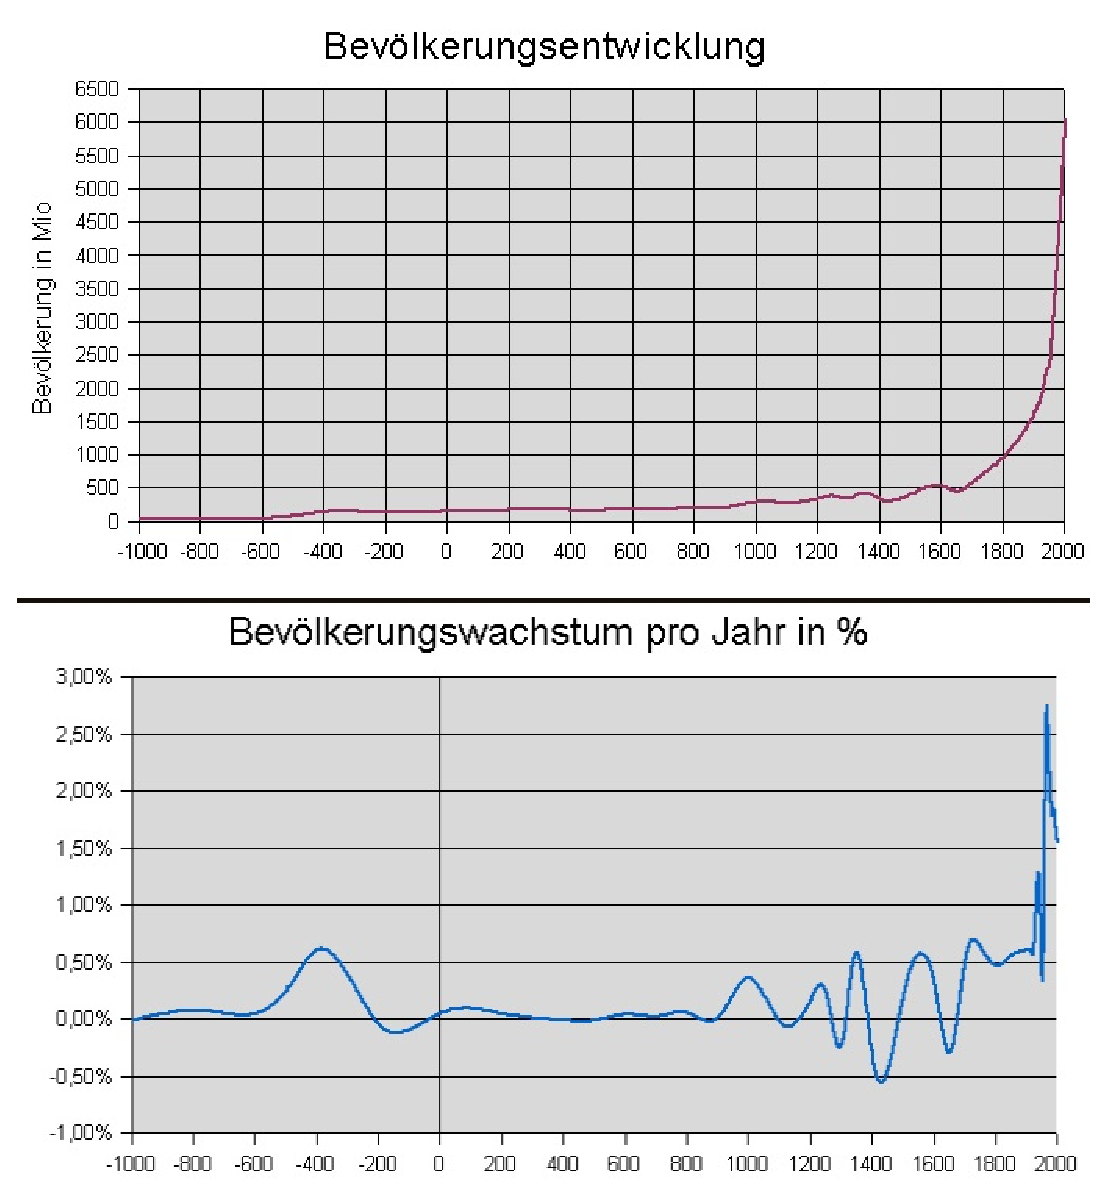
\includegraphics{../_database/Bilder/Bild24-1.eps}}
				\begin{tiny}Quelle: https://upload.wikimedia.org/wikipedia/commons/8/8a/World-pop-hist-de-2.png\end{tiny}
								
				\begin{scriptsize}Abbildung 1\end{scriptsize}
				\end{center}
				
				\meinlr{\resizebox{1\linewidth}{!}{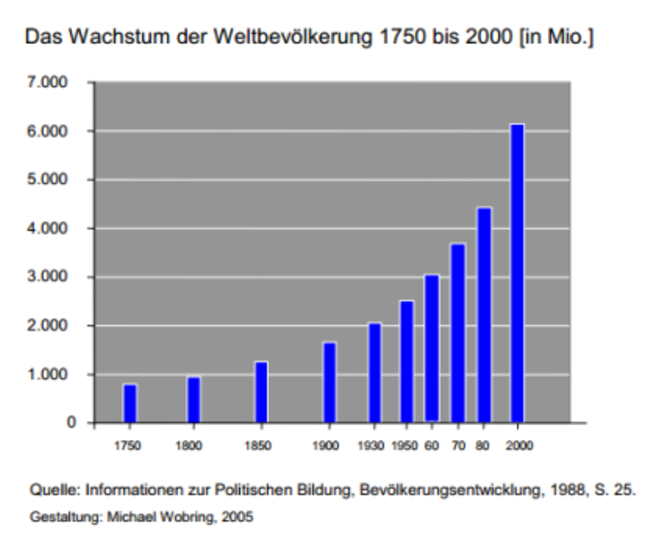
\includegraphics{../_database/Bilder/Bild24-2.eps}}
								\begin{center}\begin{scriptsize}Abbildung 2\end{scriptsize}\end{center}}{\resizebox{1.4\linewidth}{!}{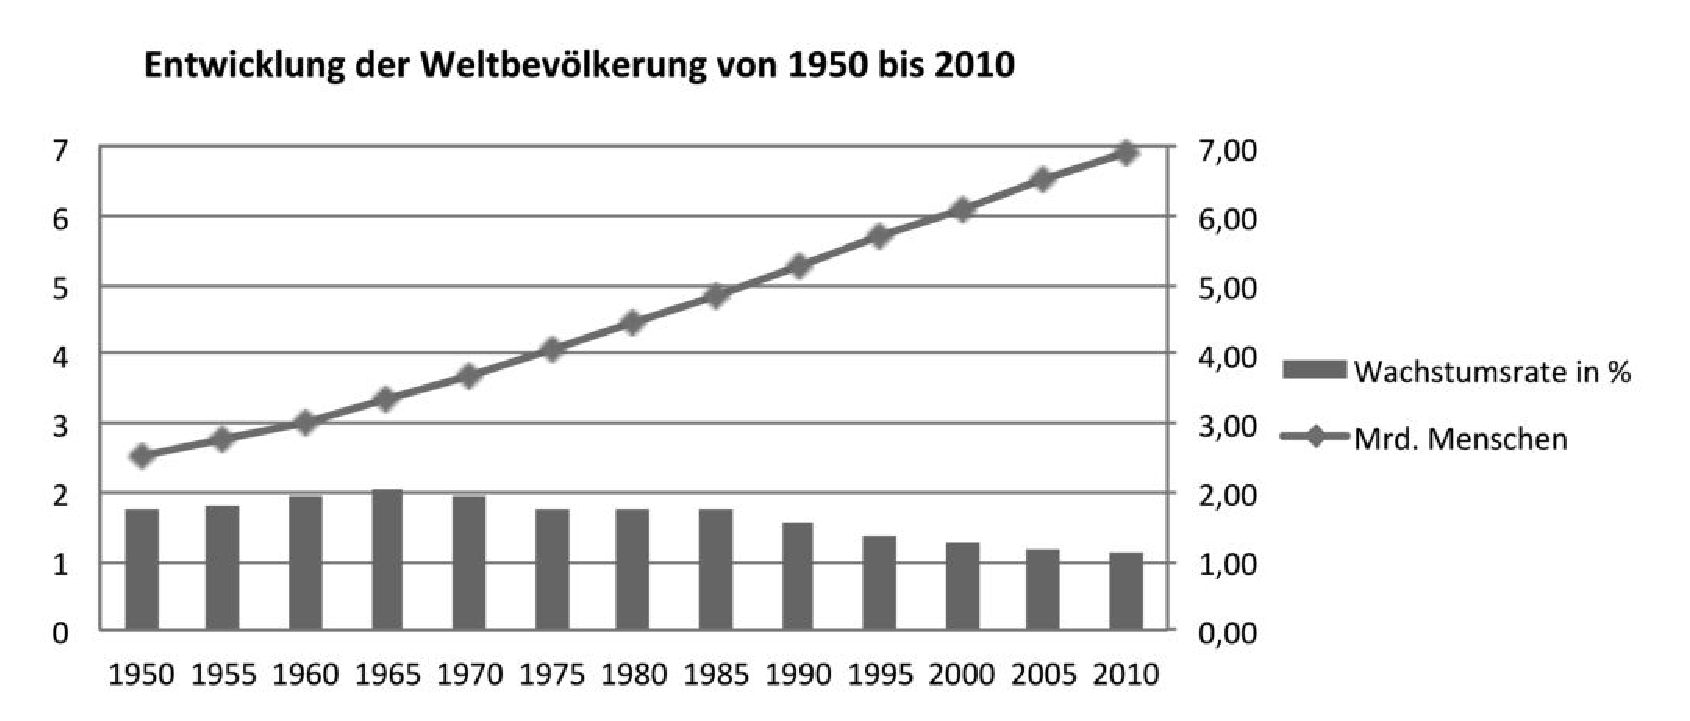
\includegraphics{../_database/Bilder/Bild24-3.eps}}
								\begin{center}\begin{scriptsize}Abbildung 3\end{scriptsize}\end{center}}\leer
								
				\begin{scriptsize}				
				\begin{tabular}{|C{1.7cm}|C{1.7cm}|C{1.7cm}|C{1.7cm}|C{1.7cm}|C{1.7cm}|C{1.7cm}|}\hline
				Jahr&Afrika&Asien&Europa&Lateinamerika&Nordamerika&Ozeanien\\ \hline
				1900&133&925&430&74&82&6\\ \hline
				1950&227&1\,403&547&167&172&13\\ \hline
				1975&419&2\,379&676&323&242&21\\ \hline
				2000&819&3\,698&727&521&319&31\\ \hline				
				\end{tabular}
				\end{scriptsize}

\subsection{Aufgabenstellung:}
\begin{enumerate}
	\item Ermittle anhand der Abbildungen, um wie viele Menschen die Weltbevölkerung von 1600 bis 18000 zugenommen hat!
	
	Nenne zwei Zeiträume, in denen die Weltbevölkerung mindesten 100 Jahre lang abgenommen hat, und begründe ihre Antwort!
	
	\item Die Weltbevölkerung hat von 1930 bis 1980 annähernd exponentiell zugenommen. Berechne unter dieser Annahme für diesen Zeitraum die jährliche Wachstumsrate auf Zehntelprozent genau!
	
	\item Begründe anhand der jährlichen Wachstumsraten aus Abbildung 3, warum die Entwicklung der Weltbevölkerung von 1950 bis 2010 nicht durch eine Exponentialfunktion beschrieben werden kann!
	
Bei konstanter Zunahme der Bevölkerungszahl ab 2010 wird für das Jahr 2050 eine Bevölkerungszahl von 10,4 Milliarden prognostiziert.\\
Berechne, von welcher jährlichen Zunahme bei dieser Prognose ausgegangen wird!
Gib die jährliche Zunahme in Millionen Menschen an!

\item Angenommen, die absoluten Zahlen der Bevölkerungsentwicklung der Kontinente und
Subkontinente im Zeitraum von 1900 bis 2000 werden in einem Säulendiagramm mit
linearer Skalierung dargestellt.\\
Begründe, warum die starke Bevölkerungszunahme in Ozeanien von 1900 bis 2000
in einem solchen Diagramm nicht erkennbar ist!

Gegeben sind fünf Aussagen zur Bevölkerungsentwicklung nach Kontinenten und Subkontinenten von 1900 bis 2000.\\
Kreuze die zutreffende(n) Aussage(n) an!\leer

\multiplechoice[5]{  %Anzahl der Antwortmoeglichkeiten, Standard: 5
				L1={Die Bevölkerung Asiens hat sich im 20. Jahrhundert annähernd
vervierfacht.},   %1. Antwortmoeglichkeit 
				L2={Seit Beginn des 20. Jahrhunderts lebten in Lateinamerika mehr
Menschen als in Nordamerika.},   %2. Antwortmoeglichkeit
				L3={Im Zeitraum von 1975 bis 2000 war die relative Bevölkerungszu-
nahme in Afrika am größten.},   %3. Antwortmoeglichkeit
				L4={In Europa war die Bevölkerungszunahme von 1975 bis 2000 ge-
ringer als von 1950 bis 1975.},   %4. Antwortmoeglichkeit
				L5={1950 lebten in Europa und Amerika zusammen bereits mehr als
eine Milliarde Menschen.},	 %5. Antwortmoeglichkeit
				L6={},	 %6. Antwortmoeglichkeit
				L7={},	 %7. Antwortmoeglichkeit
				L8={},	 %8. Antwortmoeglichkeit
				L9={},	 %9. Antwortmoeglichkeit
				%% LOESUNG: %%
				A1=1,  % 1. Antwort
				A2=3,	 % 2. Antwort
				A3=4,  % 3. Antwort
				A4=0,  % 4. Antwort
				A5=0,  % 5. Antwort
				}
						\end{enumerate}\leer
				
\antwort{\subsection{Lösungserwartung:}
\begin{enumerate}
	\item Zunahme von 1600 bis 1800: ca. 500 Millionen Menschen
	
	Die Weltbevölkerung hat mindestens 100 Jahre lang abgenommen in [250 v. Chr.; 50 v. Chr.] (bzw. $[-250;-50]$) und $[1400;1500]$, da in diesen Zeitintervallen das jährliche Bevölkerungswachstum in \% negativ ist.
	
	\item $N(t)=N_0\cdot a^t$\\
	$4,5=2\cdot a^50$\\
	$a\approx 1,016$, d.h. Zunahme um 1,6\,\% pro Jahr
	
	\item Bei einer exponentiellen Zunahme ist die jährliche Wachstumsrate konstant. Abbildung 3 zeigt, dass diese Voraussetzung im Zeitraum von 1950 bis 2010 nicht erfüllt ist.
	
	Konstante jährliche Zunahme von 2010 bis 2050:\\
	$\frac{10,4-6,9}{40}=0,0874$ Milliarden = 87,5 Millionen
	
	\item Da die Bevölkerungszahl Ozeaniens von 1900 bis 2000 jeweils weniger als 1\,\% der
Bevölkerungszahl Asiens betrug, sind die entsprechenden Säulen für Ozeanien sehr
niedrig (Höhe fast null).\\
Daher ist die Verfünffachung der Bevölkerungszahl Ozeaniens nicht erkennbar.

Lösung Multiple Choice siehe oben
			\end{enumerate}}
		\end{langesbeispiel}%
\hrule  \leer

\section{27 - MAT - AN 1.1, AN 1.3, FA 2.2, WS 1.2, WS 1.3, WS 1.1 - Kartoffeln in �sterreich - BIFIE Aufgabensammlung}

\begin{langesbeispiel} \item[0] %PUNKTE DES BEISPIELS
				Die Kartoffel ist weltweit eines der wichtigsten Nahrungsmittel.
				
				Die nachstehende Grafik zeigt die Entwicklung der Kartoffelerzeugung in �sterreich vom Jahr 2000 bis zum Jahr 2011.
				
				\begin{center}
					\textbf{Kartoffelerzeugung}
					
					\resizebox{0.8\linewidth}{!}{\psset{xunit=1.0cm,yunit=0.7cm,algebraic=true,dimen=middle,dotstyle=o,dotsize=5pt 0,linewidth=0.8pt,arrowsize=3pt 2,arrowinset=0.25}
\begin{pspicture*}(-1.366338441507557,-1.4071090537819535)(11.835465721609575,9.72757238201069)
\multips(0,0)(0,1.0){12}{\psline[linestyle=dashed,linecap=1,dash=1.5pt 1.5pt,linewidth=0.4pt,linecolor=lightgray]{c-c}(0,0)(11.835465721609575,0)}
\multips(0,0)(1.0,0){13}{\psline[linestyle=dashed,linecap=1,dash=1.5pt 1.5pt,linewidth=0.4pt,linecolor=lightgray]{c-c}(0,0)(0,9.72757238201069)}
\psaxes[labelFontSize=\scriptstyle,xAxis=true,yAxis=true,yLabels={,100, 200, 300, 400, 500, 600, 700, 800, 900},Ox=2000,Dx=1.,Dy=1.,ticksize=-2pt 0,subticks=2]{->}(0,0)(0.,0.)(11.835465721609575,9.72757238201069)
\psline[linewidth=1.2pt](0.,6.95)(1.,6.95)
\psline[linewidth=1.2pt](1.,6.95)(2.,6.84)
\psline[linewidth=1.2pt](2.,6.84)(3.,5.6)
\psline[linewidth=1.2pt](3.,5.6)(4.,6.93)
\psline[linewidth=1.2pt](4.,6.93)(5.,7.63)
\psline[linewidth=1.2pt](5.,7.63)(6.,6.55)
\psline[linewidth=1.2pt](6.,6.55)(7.,6.69)
\psline[linewidth=1.2pt](7.,6.69)(8.,7.57)
\psline[linewidth=1.2pt](8.,7.57)(9.,7.22)
\psline[linewidth=1.2pt](9.,7.22)(10.,6.72)
\psline[linewidth=1.2pt](10.,6.72)(11.,8.16)
\begin{scriptsize}
\rput[tl](-1,6){$\rotatebox{90}{\text{Menge in 1000 Tonnen}}$}
\rput[tl](0.02236339286879133,7.3){695}
\rput[tl](0.75,6.8){695}
\rput[tl](1.75,7.3){684}
\rput[tl](2.75,5.5){560}
\rput[tl](3.75,7.4){693}
\rput[tl](4.75,8){763}
\rput[tl](5.75,6.45){655}
\rput[tl](6.75,6.6){669}
\rput[tl](7.75,7.9){757}
\rput[tl](8.75,7.6){722}
\rput[tl](9.75,6.6){672}
\rput[tl](10.75,8.55){816}
\rput[tl](5.151545584806671,-0.8116715438465181){Jahr}
\end{scriptsize}
\end{pspicture*}}
				\end{center}\leer
				
				In der nachstehenden Abbildung werden Kartoffelexporte und -importe f�r den gleichen Zeitraum einander gegen�bergestellt.
				
				\begin{center}
					\textbf{Au�enhandel}
					
					\resizebox{0.8\linewidth}{!}{\newrgbcolor{qqzzff}{0. 0.6 1.}
\psset{xunit=1.0cm,yunit=0.3cm,algebraic=true,dimen=middle,dotstyle=o,dotsize=5pt 0,linewidth=0.8pt,arrowsize=3pt 2,arrowinset=0.25}
\begin{pspicture*}(-1.38,-3.449354157872534)(12.4,28.08759814267654)
\multips(0,-0)(0,5.0){7}{\psline[linestyle=dashed,linecap=1,dash=1.5pt 1.5pt,linewidth=0.4pt,linecolor=lightgray]{c-c}(0,0)(12.4,0)}
\multips(0,0)(1.0,0){14}{\psline[linestyle=dashed,linecap=1,dash=1.5pt 1.5pt,linewidth=0.4pt,linecolor=lightgray]{c-c}(0,0)(0,28.08759814267654)}
\psaxes[labelFontSize=\scriptstyle,xAxis=true,yAxis=true,yLabels={,50, 100, 150, 200, 250}, Ox=2000,Dx=1.,Dy=5.,ticksize=-2pt 0,subticks=2]{->}(0,0)(0.,0.)(12.4,28.08759814267654)
\psline[linewidth=1.2pt,linecolor=qqzzff](0.,8.4)(1.,9.1)
\psline[linewidth=1.2pt,linecolor=qqzzff](1.,9.1)(2.,12.9)
\psline[linewidth=1.2pt,linecolor=qqzzff](2.,12.9)(3.,13.5)
\psline[linewidth=1.2pt,linecolor=qqzzff](3.,13.5)(4.,11.9)
\psline[linewidth=1.2pt,linecolor=qqzzff](4.,11.9)(5.,12.8)
\psline[linewidth=1.2pt,linecolor=qqzzff](5.,12.8)(6.,16.4)
\psline[linewidth=1.2pt,linecolor=qqzzff](6.,16.4)(7.,17.7)
\psline[linewidth=1.2pt,linecolor=qqzzff](7.,17.7)(8.,15.4)
\psline[linewidth=1.2pt,linecolor=qqzzff](8.,15.4)(9.,18.2)
\psline[linewidth=1.2pt,linecolor=qqzzff](9.,18.2)(10.,19.8)
\psline[linewidth=1.2pt,linecolor=qqzzff](10.,19.8)(11.,17.2)
\psline[linewidth=1.2pt,linestyle=dashed,dash=7pt 7pt,linecolor=red](0.,7.5)(1.,6.6)
\psline[linewidth=1.2pt,linestyle=dashed,dash=7pt 7pt,linecolor=red](1.,6.6)(2.,9.)
\psline[linewidth=1.2pt,linestyle=dashed,dash=7pt 7pt,linecolor=red](2.,9.)(3.,8.2)
\psline[linewidth=1.2pt,linestyle=dashed,dash=7pt 7pt,linecolor=red](3.,8.2)(4.,10.2)
\psline[linewidth=1.2pt,linestyle=dashed,dash=7pt 7pt,linecolor=red](4.,10.2)(5.,14.8)
\psline[linewidth=1.2pt,linestyle=dashed,dash=7pt 7pt,linecolor=red](5.,14.8)(6.,13.2)
\psline[linewidth=1.2pt,linestyle=dashed,dash=7pt 7pt,linecolor=red](6.,13.2)(7.,13.2)
\psline[linewidth=1.2pt,linestyle=dashed,dash=7pt 7pt,linecolor=red](7.,13.2)(8.,17.1)
\psline[linewidth=1.2pt,linestyle=dashed,dash=7pt 7pt,linecolor=red](8.,17.1)(9.,17.2)
\psline[linewidth=1.2pt,linestyle=dashed,dash=7pt 7pt,linecolor=red](9.,17.2)(10.,16.7)
\psline[linewidth=1.2pt,linestyle=dashed,dash=7pt 7pt,linecolor=red](10.,16.7)(11.,20.8)
\psline[linewidth=1.2pt,linecolor=qqzzff](1.,24.)(2.,24.)
\psline[linewidth=1.2pt,linestyle=dashed,dash=7pt 7pt,linecolor=red](1.,22.)(2.,22.)
\begin{scriptsize}
\rput[tl](6.1,-1.8478682988602764){Jahr}
\rput[tl](0.1,9.5){\qqzzff{84}}
\rput[tl](0.85,10.5){\qqzzff{91}}
\rput[tl](1.8,14.1){\qqzzff{129}}
\rput[tl](2.8,14.6){\qqzzff{135}}
\rput[tl](3.8,13.25){\qqzzff{119}}
\rput[tl](4.8,12.5){\qqzzff{128}}
\rput[tl](5.8,17.65){\qqzzff{164}}
\rput[tl](6.8,18.7){\qqzzff{177}}
\rput[tl](7.8,15){\qqzzff{154}}
\rput[tl](8.8,19.45){\qqzzff{182}}
\rput[tl](9.8,20.8){\qqzzff{198}}
\rput[tl](10.8,16.9){\qqzzff{172}}
\rput[tl](0.1,6.9){\red{75}}
\rput[tl](0.85,6.3){\red{66}}
\rput[tl](1.85,10.1){\red{90}}
\rput[tl](2.85,8){\red{82}}
\rput[tl](3.8,9.7){\red{102}}
\rput[tl](4.8,16){\red{148}}
\rput[tl](5.8,12.9){\red{132}}
\rput[tl](6.8,12.9){\red{132}}
\rput[tl](7.8,18.2){\red{171}}
\rput[tl](8.8,16.8){\red{172}}
\rput[tl](9.8,16.5){\red{167}}
\rput[tl](10.8,21.8){\red{208}}
\rput[tl](2.4,24.5){\qqzzff{Kartoffelimporte}}
\rput[tl](2.4,22.5){\red{Kartoffelexporte}}
\rput[tl](-1.08,20.08016884761525){$\rotatebox{90}{\text{Menge in 1000 Tonnen}}$}
\end{scriptsize}
\end{pspicture*}}
					\end{center}

\subsection{Aufgabenstellung:}
\begin{enumerate}
	\item Entnehmen Sie der entsprechenden Graphik, zwischen welchen (aufeinanderfolgenden)
Jahren die absolute Zunahme (in Tonnen) und die relative Zunahme (in Prozent) der Erzeugung im Vergleich zum Vorjahr jeweils am gr��ten war! Gib die entsprechenden
Werte an!

Im vorliegenden Fall fand die gr��te relative Zunahme der Erzeugung in einem anderen
Zeitintervall statt als die gr��te absolute Zunahme.\\
Gib eine mathematische Begr�ndung an, warum die gr��te relative Zunahme und
die gr��te absolute Zunahme einer Gr��e oder eines Prozesses nicht im gleichen Zeitintervall stattfinden m�ssen!

\item Berechne und interpretiere den Ausdruck $\frac{E_{2011}-E_{2000}}{11}$, wobei $E_\text{Jahr}$ die Exportmenge in einem Kalenderjahr angibt! Gib bei der Interpretation auch die entsprechende Einheit an.

Die Exportentwicklung von 2000 bis 2011 soll durch eine lineare Funktion $f$ approximiert
werden, wobei die Variable t die Anzahl der seit 2000 vergangenen Jahre sein soll. Die
Funktionswerte f�r die Jahre 2000 und 2011 sollen dabei mit den in der Graphik angef�hrten Werten �bereinstimmen. Gib eine Gleichung dieser Funktion $f$ an!

\item Stelle in der nachstehenden Abbildung die Differenz "`Export minus Import"' der Mengen an Kartoffeln f�r die Jahre 2003 bis 2009 in einem S�ulendiagramm dar!
	
	\begin{center}
					\textbf{Saldo Export-Import}
					
					\resizebox{0.8\linewidth}{!}{\psset{xunit=1.4cm,yunit=0.05cm,algebraic=true,dimen=middle,dotstyle=o,dotsize=5pt 0,linewidth=0.8pt,arrowsize=3pt 2,arrowinset=0.25}
\begin{pspicture*}(-1,-69.33333333333154)(7.151969309462931,66.39999999999834)
\multips(0,-60)(0,4.0){34}{\psline[linestyle=dashed,linecap=1,dash=1.5pt 1.5pt,linewidth=0.4pt,linecolor=lightgray]{c-c}(0,0)(7.151969309462931,0)}
\multips(0,0)(100.0,0){1}{\psline[linestyle=dashed,linecap=1,dash=1.5pt 1.5pt,linewidth=0.4pt,linecolor=lightgray]{c-c}(0,-60)(0,66.39999999999834)}
\psaxes[labelFontSize=\scriptstyle,xAxis=true,yAxis=true,labels=y,Dx=1.,Dy=20.,ticksize=-2pt 0,subticks=2]{->}(0,0)(0.,-60)(7.151969309462931,66.39999999999834)
\antwort{\pspolygon[linecolor=blue,fillcolor=blue,fillstyle=solid,opacity=0.5](0.2,0.)(0.2,-53.)(0.8,-53.)(0.8,0.)
\pspolygon[linecolor=blue,fillcolor=blue,fillstyle=solid,opacity=0.5](1.2,0.)(1.2,-17.)(1.8,-17.)(1.8,0.)
\pspolygon[linecolor=blue,fillcolor=blue,fillstyle=solid,opacity=0.5](2.2,0.)(2.2,20.)(2.8,20.)(2.8,0.)
\pspolygon[linecolor=blue,fillcolor=blue,fillstyle=solid,opacity=0.5](3.2,0.)(3.2,-32.)(3.8,-32.)(3.8,0.)
\pspolygon[linecolor=blue,fillcolor=blue,fillstyle=solid,opacity=0.5](4.2,0.)(4.2,-45.)(4.8,-45.)(4.8,0.)
\pspolygon[linecolor=blue,fillcolor=blue,fillstyle=solid,opacity=0.5](5.2,0.)(5.2,17.)(5.8,17.)(5.8,0.)
\pspolygon[linecolor=blue,fillcolor=blue,fillstyle=solid,opacity=0.5](6.2,0.)(6.2,-10.)(6.8,-10.)(6.8,0.)}
\begin{scriptsize}
\rput[tl](0.3,-3.1999999999998883){2003}
\rput[tl](1.3,-3.1999999999998883){2004}
\rput[tl](2.3,-3.1999999999998883){2005}
\rput[tl](3.3,-3.1999999999998883){2006}
\rput[tl](4.3,-3.1999999999998883){2007}
\rput[tl](5.3,-3.1999999999998883){2008}
\rput[tl](6.3,-3.1999999999998883){2009}
\rput[tl](3,-63){Jahr}
\rput[tl](-0.8,26.93333333333268){$\rotatebox{90}{\text{Saldo in 1000 Tonnen}}$}
\end{scriptsize}
\end{pspicture*}}
\end{center}

Berechne das arithmetische Mittel dieser Differenz f�r die genannten Jahre!

\item Ein Index ist eine statistische Kennziffer, um die Entwicklung von Gr��en im Zeitverlauf darzustellen. Oft wird der Ausgangswert mit dem Basiswert 100 versehen. Ein Index von 120 bedeutet beispielsweise, dass eine Gr��e seit dem Basiszeitpunkt um 20\,\% gestiegen ist.

Die nachstehende Graphik zeigt die Entwicklung der in �sterreich verzehrten Kartoffelmenge (Nahrungsverbrauch) bezogen auf das Jahr 2000.

\begin{center}
					\textbf{Nahrungsverbrauch}
					
					\resizebox{0.8\linewidth}{!}{\psset{xunit=1.6cm,yunit=0.8cm,algebraic=true,dimen=middle,dotstyle=o,dotsize=5pt 0,linewidth=0.8pt,arrowsize=3pt 2,arrowinset=0.25}
\begin{pspicture*}(-0.8674067054466462,-1.1184701870029385)(6.267692353635041,8.521136170252973)
\multips(0,0)(0,1.0){10}{\psline[linestyle=dashed,linecap=1,dash=1.5pt 1.5pt,linewidth=0.4pt,linecolor=lightgray]{c-c}(0,0)(7.267692353635041,0)}
\multips(0,0)(100.0,0){1}{\psline[linestyle=dashed,linecap=1,dash=1.5pt 1.5pt,linewidth=0.4pt,linecolor=lightgray]{c-c}(0,0)(0,8.521136170252973)}
\psaxes[labelFontSize=\scriptstyle,xAxis=true,yAxis=true,labels=y,yLabels={,\text{94,0}, \text{96,0},\text{98,0},\text{100,0},\text{102,0},\text{104,0},\text{106,0},\text{108,0},\text{110,0}},Dx=1.,Dy=1.,ticksize=-2pt 0,subticks=2]{->}(0,0)(0.,0.)(6.267692353635041,8.521136170252973)
\pspolygon[linecolor=blue,fillcolor=blue,fillstyle=solid,opacity=1.0](0.25,0.)(0.25,3.)(0.5,3.)(0.5,0.)
\pspolygon[linecolor=red,fillcolor=red,fillstyle=solid,opacity=1.0](0.75,0.)(0.5,0.)(0.5,3.)(0.75,3.)
\pspolygon[linecolor=blue,fillcolor=blue,fillstyle=solid,opacity=1.0](1.25,0.)(1.25,5.1)(1.5,5.1)(1.5,0.)
\pspolygon[linecolor=red,fillcolor=red,fillstyle=solid,opacity=1.0](1.5,5.15)(1.75,5.15)(1.75,0.)(1.5,0.)
\pspolygon[linecolor=blue,fillcolor=blue,fillstyle=solid,opacity=1.0](2.25,0.)(2.25,4.)(2.5,4.)(2.5,0.)
\pspolygon[linecolor=red,fillcolor=red,fillstyle=solid,opacity=1.0](2.5,0.)(2.5,3.4)(2.75,3.4)(2.75,0.)
\pspolygon[linecolor=blue,fillcolor=blue,fillstyle=solid,opacity=1.0](3.25,0.)(3.25,3.9)(3.5,3.9)(3.5,0.)
\pspolygon[linecolor=red,fillcolor=red,fillstyle=solid,opacity=1.0](3.5,0.)(3.5,2.8)(3.75,2.8)(3.75,0.)
\pspolygon[linecolor=blue,fillcolor=blue,fillstyle=solid,opacity=1.0](4.25,0.)(4.25,7.2)(4.5,7.2)(4.5,0.)
\pspolygon[linecolor=red,fillcolor=red,fillstyle=solid,opacity=1.0](4.5,0.)(4.5,5.6)(4.75,5.6)(4.75,0.)
\pspolygon[linecolor=blue,fillcolor=blue,fillstyle=solid,opacity=1.0](5.25,0.)(5.25,6.05)(5.5,6.05)(5.5,0.)
\pspolygon[linecolor=red,fillcolor=red,fillstyle=solid,opacity=1.0](5.5,0.)(5.5,4.2)(5.75,4.2)(5.75,0.)
\pspolygon[linecolor=blue,fillcolor=blue,fillstyle=solid,opacity=1.0](0.25,8.)(0.25,7.5)(0.5,7.5)(0.5,8.)
\pspolygon[linecolor=red,fillcolor=red,fillstyle=solid,opacity=1.0](0.25,7.)(0.25,6.5)(0.5,6.5)(0.5,7.)
\begin{scriptsize}
\rput[tl](0.63,7.85){Nahrungsverbrauch}
\rput[tl](0.63,6.85){Nahrungsverbrauch pro Kopf}
\rput[tl](-0.8,6.949255369364486){$\rotatebox{90}{\text{Index bezogen auf das Jahr 2000}}$}
\rput[tl](3,-0.7){Jahr}
\rput[tl](0.3,-0.15){2000}
\rput[tl](1.3,-0.15){2002}
\rput[tl](2.3,-0.15){2004}
\rput[tl](3.3,-0.15){2006}
\rput[tl](4.3,-0.15){2008}
\rput[tl](5.3,-0.15){2010}
\end{scriptsize}
\end{pspicture*}}
\end{center}

Geben Sie jeweils ein Jahr an, in dem die Einwohnerzahl in �sterreich h�her bzw. niedriger
war als im Jahr 2000! Begr�nde deine Antwort!

Zeichne in die nachstehende Graphik zwei m�gliche S�ulen f�r ein Jahr, in dem der
absolute Nahrungsverbrauch niedriger und die Bev�lkerungszahl h�her war als im
Jahr 2000!

\begin{center}
					\textbf{Nahrungsverbrauch}
					
					\resizebox{0.8\linewidth}{!}{\psset{xunit=5cm,yunit=0.8cm,algebraic=true,dimen=middle,dotstyle=o,dotsize=5pt 0,linewidth=0.8pt,arrowsize=3pt 2,arrowinset=0.25}
\begin{pspicture*}(-0.35,-1.1184701870029385)(2.267692353635041,11.521136170252973)
\multips(0,0)(0,1.0){12}{\psline[linestyle=dashed,linecap=1,dash=1.5pt 1.5pt,linewidth=0.4pt,linecolor=lightgray]{c-c}(0,0)(7.267692353635041,0)}
\multips(0,0)(100.0,0){1}{\psline[linestyle=dashed,linecap=1,dash=1.5pt 1.5pt,linewidth=0.4pt,linecolor=lightgray]{c-c}(0,0)(0,8.521136170252973)}
\psaxes[labelFontSize=\scriptstyle,xAxis=true,yAxis=true,labels=y,yLabels={,\text{0,0}, \text{20,0},\text{40,0},\text{60,0},\text{80,0},\text{100,0},\text{120,0},\text{140,0},\text{160,0},\text{180,0},\text{200,0}},Dx=1.,Dy=1.,ticksize=-2pt 0]{->}(0,0)(0.,0.)(2.267692353635041,11.521136170252973)
\pspolygon[linecolor=blue,fillcolor=blue,fillstyle=solid,opacity=1.0](0.25,0.)(0.25,3.)(0.5,3.)(0.5,0.)
\pspolygon[linecolor=red,fillcolor=red,fillstyle=solid,opacity=1.0](0.75,0.)(0.5,0.)(0.5,3.)(0.75,3.)

\pspolygon[linecolor=blue,fillcolor=blue,fillstyle=solid,opacity=1.0](0.25,11.)(0.25,10.5)(0.35,10.5)(0.35,11.)
\pspolygon[linecolor=red,fillcolor=red,fillstyle=solid,opacity=1.0](0.25,10.)(0.25,9.5)(0.35,9.5)(0.35,10.)
\begin{scriptsize}
\rput[tl](0.4,10.85){Nahrungsverbrauch}
\rput[tl](0.4,9.85){Nahrungsverbrauch pro Kopf}
\rput[tl](-0.25,7.6){$\rotatebox{90}{\text{Index bezogen auf das Jahr 2000}}$}
\rput[tl](1,-0.4){Jahr}
\rput[tl](0.44,-0.15){2000}
\rput[tl](1.44,-0.15){2002}
\end{scriptsize}
\end{pspicture*}}
\end{center}
						\end{enumerate}\leer
				
\antwort{\subsection{L�sungserwartung:}
\begin{enumerate}
	\item absolute Zunahme zwischen 2003 und 2004: 133 000 Tonnen\\
absolute Zunahme zwischen 2010 und 2011: 144 000 Tonnen\\
Die gr��te absolute Zunahme war im Zeitintervall von 2010 bis 2011.\\
relative Zunahme zwischen 2003 und 2004: 23,75\,\%\\
L�sungsintervall in Prozent: $[23; 24]$\\
relative Zunahme zwischen 2010 und 2011: ca. 21,43\,\%\\
L�sungsintervall in Prozent: $[21; 22]$
Die gr��te relative Zunahme war zwischen 2003 und 2004.\\
Da f�r die Berechnung der relativen Zunahme einer Gr��e auch der Bezugswert entscheidend ist, m�ssen gr��te absolute Zunahme und gr��te relative Zunahme einer Gr��e oder
eines Prozesses nicht im gleichen Zeitintervall stattfinden. �quivalente Formulierungen sind
ebenfalls als richtig zu werten.

\item $\frac{E_{2011}-E_{2000}}{11}\approx 12\,000$ Tonnen pro Jahr.

Die durchschnittliche Zunahme des �sterreichischen Kartoffelexports betr�gt
ca. 12 000 Tonnen pro Jahr.\\
L�sungsintervall: $[12 000; 12 100]$
Die richtige Einheit muss in der Interpretation vorhanden sein.\\
$f$ mit $f(t)=75000+12000\cdot t$ oder $f(t)=75+12\cdot t$ oder $f(t)=\frac{133}{11}\cdot t+75$
Jede j�hrliche Zunahme aus dem oben angef�hrten L�sungsintervall muss akzeptiert werden.

\item L�sung Grafik siehe oben

Genauigkeit der S�ulenl�ngen: Toleranzbereich $\pm 5\,000$ Tonnen

arithmetisches Mittel: $\frac{-53-17+20-32-45+17-10}{7}\approx -17$

L�sungsintervall: bei Berechnung in 1\,000 Tonnen: $[-18; -16]$; bei Berechnung in Tonnen:
$[-18\,000; -16\,000]$
	
\item \begin{itemize}
	\item niedrigere Einwohnerzahl (als im Jahr 2000) in den Jahren: 2002 (prozentuelle Ver�nderung des Nahrungsverbrauchs kleiner als jene des Nahrungsverbrauchs pro Kopf)
\item h�here Einwohnerzahl (als im Jahr 2000) in den Jahren: 2004, 2006, 2008 und 2010
(prozentuelle Ver�nderung des Nahrungsverbrauchs gr��er als jene des Nahrungsverbrauchs pro Kopf)
\end{itemize}
Die Angabe eines Jahres ist hier ausreichend.

Die S�ule f�r den gesamten Nahrungsverbrauch muss niedriger sein als die S�ule f�r
100\% im Jahr 2000. Die S�ule f�r den Nahrungsverbrauch pro Kopf muss bei einer steigenden Bev�lkerungszahl niedriger als die S�ule f�r den gesamten Nahrungsverbrauch
sein.
			\end{enumerate}}
		\end{langesbeispiel}%
\hrule  \leer

\section{30 - MAT - AG 2.1, FA 4.1, FA 4.3, FA 5.1, FA 5.6, AN 1.1, AN 1.4, WS 1.3 - Waldbewirtschaftung - BIFIE Aufgabensammlung}

\begin{langesbeispiel} \item[0] %PUNKTE DES BEISPIELS
				Der Holzbestand eines durchschnittlichen Fichtenwaldes in Österreich beträgt $350\,m^3$ pro Hektar Waldfläche. Pro Jahr ist mit einem durchschnittlichen Zuwachs von $3,3\,\%$ zu rechnen. Bei einer nachhaltigen Bewirtschaftung, wie sie in Österreich vorgeschrieben ist, soll der Holzbestand des Waldes gleich bleiben oder leicht zunehmen.
				
Der nachstehenden Grafik kann die Entwicklung des Holzpreises bei Fichtenholz im Zeitraum von 1995 bis 2011 entnommen werden.

\begin{center}
\subsection{Holzpreis bei Fichtenholz in \euro$/m^3$}
\resizebox{1\linewidth}{!}{\psset{xunit=2.3cm,yunit=0.25cm,algebraic=true,dimen=middle,dotstyle=o,dotsize=5pt 0,linewidth=0.8pt,arrowsize=3pt 2,arrowinset=0.25}
\begin{pspicture*}(-0.82,-3.166666666666629)(9.52,49.66666666666655)
\multips(0,0)(0,2.0){27}{\psline[linestyle=dashed,linecap=1,dash=1.5pt 1.5pt,linewidth=0.4pt,linecolor=lightgray]{c-c}(0,0)(9.52,0)}
\multips(0,0)(100.0,0){1}{\psline[linestyle=dashed,linecap=1,dash=1.5pt 1.5pt,linewidth=0.4pt,linecolor=lightgray]{c-c}(0,0)(0,49.66666666666655)}
\psaxes[labelFontSize=\scriptstyle,xAxis=true,yAxis=true,labels=y,Oy=50,Dy=2.,ticksize=-2pt 0,subticks=2]{->}(0,0)(0.,0.)(9.52,49.66666666666655)
\rput[tl](0.06,48.749999999999886){\euro$/m^3$}
\rput[tl](8.42,2.){Jahr}
\psline[linewidth=1.2pt](0.5,26.)(1.,14.)
\psline[linewidth=1.2pt](1.,14.)(1.5,23.)
\psline[linewidth=1.2pt](1.5,23.)(2.,28.)
\psline[linewidth=1.2pt](2.,28.)(2.5,29.)
\psline[linewidth=1.2pt](2.5,29.)(3.,23.)
\psline[linewidth=1.2pt](3.,23.)(3.5,23.)
\psline[linewidth=1.2pt](3.5,23.)(4.,24.)
\psline[linewidth=1.2pt](4.,24.)(4.5,16.)
\psline[linewidth=1.2pt](4.5,16.)(5.,18.)
\psline[linewidth=1.2pt](5.,18.)(5.5,19.)
\psline[linewidth=1.2pt](5.5,19.)(6.,26.)
\psline[linewidth=1.2pt](6.,26.)(6.5,26.)
\psline[linewidth=1.2pt](6.5,26.)(7.,19.)
\psline[linewidth=1.2pt](7.,19.)(7.5,20.)
\psline[linewidth=1.2pt](7.5,20.)(8.,39.)
\psline[linewidth=1.2pt](8.,39.)(8.5,44.)
\begin{scriptsize}
\psdots[dotsize=4pt 0,dotstyle=square*,dotangle=45](0.5,26.)
\psdots[dotsize=4pt 0,dotstyle=square*,dotangle=45](1.,14.)
\psdots[dotsize=4pt 0,dotstyle=square*,dotangle=45](1.5,23.)
\psdots[dotsize=4pt 0,dotstyle=square*,dotangle=45](2.,28.)
\psdots[dotsize=4pt 0,dotstyle=square*,dotangle=45](2.5,29.)
\psdots[dotsize=4pt 0,dotstyle=square*,dotangle=45](3.,23.)
\psdots[dotsize=4pt 0,dotstyle=square*,dotangle=45](3.5,23.)
\psdots[dotsize=4pt 0,dotstyle=square*,dotangle=45](4.,24.)
\psdots[dotsize=4pt 0,dotstyle=square*,dotangle=45](4.5,16.)
\psdots[dotsize=4pt 0,dotstyle=square*,dotangle=45](5.,18.)
\psdots[dotsize=4pt 0,dotstyle=square*,dotangle=45](5.5,19.)
\psdots[dotsize=4pt 0,dotstyle=square*,dotangle=45](6.,26.)
\psdots[dotsize=4pt 0,dotstyle=square*,dotangle=45](6.5,26.)
\psdots[dotsize=4pt 0,dotstyle=square*,dotangle=45](7.,19.)
\psdots[dotsize=4pt 0,dotstyle=square*,dotangle=45](7.5,20.)
\psdots[dotsize=4pt 0,dotstyle=square*,dotangle=45](8.,39.)
\psdots[dotsize=4pt 0,dotstyle=square*,dotangle=45](8.5,44.)
\rput[tl](-0.18,-1){1994}
\rput[tl](0.82,-1){1996}
\rput[tl](1.82,-1){1998}
\rput[tl](2.82,-1){2000}
\rput[tl](3.82,-1){2002}
\rput[tl](4.82,-1){2004}
\rput[tl](5.82,-1){2006}
\rput[tl](6.82,-1){2008}
\rput[tl](7.82,-1){2010}
\rput[tl](8.82,-1){2012}
\end{scriptsize}
\end{pspicture*}}
\end{center}

\subsection{Aufgabenstellung:}
\begin{enumerate}
	\item Bestimme das maximale Holzvolumen (in $m^3/ha$), das bei einer nachhaltigen Bewirtschaftung pro Jahr geschlägert werden darf!
	
Berechne, um wie viel Prozent der Holzbestand eines durchschnittlichen Fichtenwaldes innerhalb von 10 Jahren zunimmt, unter der Annahme, dass keinerlei Schlägerungen vorgenommen werden, alle anderen genannten Rahmenbedingungen jedoch unverändert bleiben!

\item Der Holzbestand eines 20 ha großen Fichtenwaldes wird in einem Zeitraum von 15 Jahren jährlich jeweils am Ende des Jahres (nachdem der jährliche Zuwachs abgeschlossen ist) um 10 $m^3$ pro Hektar (also um 200 $m^3$) verringert.

Ermitteln Sie den Holzbestand des Fichtenwaldes nach Ablauf von 15 Jahren!

Gib an, ob bei dieser Art der Bewirtschaftung der Holzbestand des Fichtenwaldes trotz Schlägerung exponentiell zunimmt, und begründe deine Entscheidung!
	
\item Ermittel für den Zeitraum 2003 bis 2011 die empirische Standardabweichung des Holzpreises entsprechend der Formel

$$\sigma=\sqrt{\frac{1}{n-1}\cdot\sum^n_{i=1}({x_i-\overline{x})^2}}$$

Dabei werden mit $x_i$ die Beobachtungswerte und mit $\overline{x}$ das arithmetische Mittel der Beobachtungswerte bezeichnet. Lies die dazu notwendigen Daten aus der Grafik ab!

Begründen Sie anhand der Grafik, warum die empirische Standardabweichung des
Holzpreises für den Zeitraum 1998 bis 2004 kleiner ist als die empirische Standardabweichung für den Zeitraum 2005 bis 2011!

\item Die Entwicklung des Holzpreises soll für den Zeitraum von 2009 bis 2011 durch eine Funktion $P$ mit $P(t)=a\cdot t^2+b\cdot t+c$ mit $a,b,c\in\mathbb{R}$ und $a\neq 0$ modelliert werden. Der Holzpreis $P(t)$ wird in \euro$/m^3$ angegeben, die Zeitrechnung beginnt mit dem Jahr 2009 und erfolgt in der Einheit "`Jahre"'.

Führe die Modellierung auf Basis der Daten für die Jahre 2009, 2010 und 2011 durch und begründe, warum der Parameter $a$ negativ sein muss!

Ermittle eine Prognose für den in der Grafik nicht angegebenen Holzpreis für das Jahr 2012 mithilfe dieser Modellfunktion!

\item Bestimme für den Zeitraum von 1995 bis 2011 die absoluten Holzpreisänderungen aufeinanderfolgender Jahre!

Gib dasjenige Intervall [Jahr 1; Jahr 2] an, in dem sich der Holzpreis prozentuell am stärksten ändert!
						\end{enumerate}\leer
				
\antwort{\subsection{Lösungserwartung:}
\begin{enumerate}
	\item $350\cdot 0,033=11,55$\\
	Jährlich dürfen bei einer nachhaltigen Bewirtschaftung maximal 11,55 $m^3$/ha Holz geschlägert werden.
	
	$1,033^{10}\approx 1,384$\\
	Unter der Annahme, dass keine Schlägerungen erfolgen, nimmt der Holzbestand innerhalb von zehn Jahren um ca. 38,4\,\% zu.
	
	\item Tabelle:
	
	\begin{tabular}{|c|c|}\hline
	Jahr&Holzbestand in $m^3$\\ \hline
	0&7\,000\\ \hline
	1&7\,031\\ \hline
	2&7\,063,023\\ \hline
	3&7\,096,102759\\ \hline
4&7\,130,27415\\ \hline
5&7\,165,573197\\ \hline
6&7\,202,037112\\ \hline
7&7\,239,704337\\ \hline
8&7\,278,61458\\ \hline
9&7\,318,808861\\ \hline
10&7\,360,329554\\ \hline
11&7\,403,220429\\ \hline
12&7\,447,526703\\ \hline
13&7\,493,295085\\ \hline
14&7\,540,573822\\ \hline
15&7\,589,412759\\ \hline
	\end{tabular}\leer
	
	Wenn der Holzbestand eines 20 ha großen Fichtenwaldes jährlich jeweils am Ende des Jahres um 10 $m^3$ pro Hektar verringert wird, beträgt er nach Ablauf von 15 Jahren ca. 7 589,41 $m^3$.
	
Bei dieser Art der Bewirtschaftung nimmt der Holzbestand nicht exponentiell zu, da das jährliche prozentuelle Wachstum nicht konstant ist.

\item Die empirische Standardabweichung beträgt ca. 9,91 \euro$/m^3$.

Im Zeitraum von 1998 bis 2004 ist die empirische Standardabweichung des Holzpreises kleiner als im Zeitraum von 2005 bis 2011, da die Schwankungen der Werte des Holzpreises im Zeitraum von 1998 bis 2004 geringer sind.

\item $P(t)=-7\cdot t^2+26\cdot t+70$

\begin{center}
	\subsection{Holzpreis in \euro$/m^3$}
	
	\resizebox{0.8\linewidth}{!}{\psset{xunit=5cm,yunit=0.09cm,algebraic=true,dimen=middle,dotstyle=o,dotsize=5pt 0,linewidth=0.8pt,arrowsize=3pt 2,arrowinset=0.25}
\begin{pspicture*}(-0.2473684210526314,-12.595999999999828)(2.9368421052631564,109.31528571428521)
\multips(0,0)(0,10.0){13}{\psline[linestyle=dashed,linecap=1,dash=1.5pt 1.5pt,linewidth=0.4pt,linecolor=lightgray]{c-c}(0,0)(2.9368421052631564,0)}
\multips(0,0)(10.0,0){1}{\psline[linestyle=dashed,linecap=1,dash=1.5pt 1.5pt,linewidth=0.4pt,linecolor=lightgray]{c-c}(0,0)(0,109.31528571428521)}
\psaxes[labelFontSize=\scriptstyle,xAxis=true,yAxis=true,Dx=0.5,Dy=10.,ticksize=-2pt 0,subticks=2]{->}(0,0)(0.,0.)(2.9368421052631564,109.31528571428521)
\psplot[linewidth=1.2pt,plotpoints=200]{0}{2}{-7.0*x^(2.0)+26.0*x+70.0}
\rput[tl](1.2052631578947361,-5.9){Jahre ab 2009}
\rput[tl](0.10526315789473682,104.36685714285666){$y=-7x^2+26x+70$}
\rput[tl](0.32631578947368406,95.19349999999955){$R^2=1$}
\begin{scriptsize}
\psdots[dotsize=4pt 0,dotstyle=square*,dotangle=45](0.,70.)
\psdots[dotsize=4pt 0,dotstyle=square*,dotangle=45](1.,89.)
\psdots[dotsize=4pt 0,dotstyle=square*,dotangle=45](2.,94.)
\end{scriptsize}
\end{pspicture*}}
\end{center}\leer

Der Wert des Parameters $a$ muss negativ sein, weil der Graph der Modellfunktion eine nach unten geöffnete Parabel ist.

Prognosewert für das Jahr 2012:\\
$P(3)=85\,$\euro$/m^3$

\item Tabelle:

\begin{tabular}{|c|c|c|c|}\hline
Jahr&Holzpreis in \euro$/m^3$&absolute Änderungen&prozentuelle Änderungen\\ \hline
1995&76& & \\ \hline
1996&64&-12&-15,79\\ \hline
1997&73&9&14,06\\ \hline
1998&78&5&6,85\\ \hline
1999&79&1&1,28\\ \hline
2000&73&-6&-7,59\\ \hline
2001&73&0&0\\ \hline
2002&74&1&1,37\\ \hline
2003&66&-8&-10,81\\ \hline
2004&68&2&3,03\\ \hline
2005&69&1&1,47\\ \hline
2006&76&7&10,14\\ \hline
2007&76&0&0\\ \hline
2008&69&-7&-9,21\\ \hline
2009&70&1&1,45\\ \hline
2010&89&19&27,14\\ \hline
2011&94&5&5,62\\ \hline
\end{tabular}\leer

Im Zeitraum $[2009; 2010]$ ändert sich der Holzpreis prozentuell am stärksten.
	\end{enumerate}}
		\end{langesbeispiel}%
\hrule  \leer

\section{31 - MAT - WS 1.1, WS 1.3 - Hallenbad - Matura 2013/14 Haupttermin}

\begin{langesbeispiel} \item[0] %PUNKTE DES BEISPIELS
				Das �rtliche Hallenbad einer kleinen Gemeinde ver�ffentlicht Anfang 2008 in der Gemeindezeitschrift eine Statistik �ber die j�hrlichen Besucherzahlen und die Anzahl der offenen Tage f�r die letzten acht Jahre:
					
					\resizebox{1\linewidth}{!}{\begin{tabular}{|l|c|c|c|c|c|c|c|c|}\hline
					Jahr&2000&2001&2002&2003&2004&2005&2006&2007\\ \hline
					Besucherzahlen&33\,200&32\,500&34\,000&33\,500&33\,200&33\,100&32\,900&32\,500\\ \hline
					offene Tage&197&192&200&195&193&190&186&180\\ \hline
					\end{tabular}}

Das Hallenbad bedarf einer Renovierung. Im Gemeinderat steht nun die Entscheidung an, ob Geld in das Hallenbad investiert oder das Hallenbad geschlossen werden soll. Im Vorfeld der Entscheidung ver�ffentlichen zwei �rtliche Gemeinderatsparteien - Partei $A$ und Partei $B$ - folgende Diagramme in ihren Parteizeitschriften:

\begin{center}
\textbf{Besucherzahlen 2000-2007}\leer

\resizebox{0.5\linewidth}{!}{\psset{xunit=1.0cm,yunit=0.15cm,algebraic=true,dimen=middle,dotstyle=o,dotsize=5pt 0,linewidth=0.8pt,arrowsize=3pt 2,arrowinset=0.25}
\begin{pspicture*}(-1.6848,-4.089123900293161)(8.8938,44.10412206744805)
\multips(0,0)(0,5.0){10}{\psline[linestyle=dashed,linecap=1,dash=1.5pt 1.5pt,linewidth=0.4pt,linecolor=lightgray]{c-c}(0,0)(8.8938,0)}
\multips(0,0)(1.0,0){11}{\psline[linestyle=dashed,linecap=1,dash=1.5pt 1.5pt,linewidth=0.4pt,linecolor=lightgray]{c-c}(0,0)(0,44.10412206744805)}
\psaxes[labelFontSize=\scriptstyle,xAxis=true,yAxis=true,showorigin=false,ylabelFactor={\,000}, Ox=1999,Dx=1.,Dy=5.,ticksize=-2pt 0,subticks=2]{->}(0,0)(0.,0.)(8.8938,44.10412206744805)
\psline(1.,33.2)(2.,32.5)
\psline(2.,32.5)(3.,34.)
\psline(3.,34.)(4.,33.5)
\psline(4.,33.5)(5.,33.2)
\psline(5.,33.2)(6.,33.1)
\psline(6.,33.1)(7.,32.9)
\psline(7.,32.9)(8.,32.5)
\begin{scriptsize}
\psdots[dotsize=3pt 0,dotstyle=square*,dotangle=45](1.,33.2)
\psdots[dotsize=3pt 0,dotstyle=square*,dotangle=45](2.,32.5)
\psdots[dotsize=3pt 0,dotstyle=square*,dotangle=45](3.,34.)
\psdots[dotsize=3pt 0,dotstyle=square*,dotangle=45](4.,33.5)
\psdots[dotsize=3pt 0,dotstyle=square*,dotangle=45](5.,33.2)
\psdots[dotsize=3pt 0,dotstyle=square*,dotangle=45](6.,33.1)
\psdots[dotsize=3pt 0,dotstyle=square*,dotangle=45](7.,32.9)
\psdots[dotsize=3pt 0,dotstyle=square*,dotangle=45](8.,32.5)
\end{scriptsize}
\end{pspicture*}}

\textit{Partei $A$}
\end{center}

\begin{center}
\textbf{Besucherzahlen 2000-2007}\leer

\resizebox{0.5\linewidth}{!}{\psset{xunit=1.0cm,yunit=2cm,algebraic=true,dimen=middle,dotstyle=o,dotsize=5pt 0,linewidth=0.8pt,arrowsize=3pt 2,arrowinset=0.25}
\begin{pspicture*}(0,31.9)(8.8938,34.4)
\multips(0,32.2)(0,0.4){10}{\psline[linestyle=dashed,linecap=1,dash=1.5pt 1.5pt,linewidth=0.4pt,linecolor=lightgray]{c-c}(2,0)(8.8938,0)}
\multips(2,0)(1.0,0){11}{\psline[linestyle=dashed,linecap=1,dash=1.5pt 1.5pt,linewidth=0.4pt,linecolor=lightgray]{c-c}(0,32.2)(0,44.10412206744805)}
\psaxes[labelFontSize=\scriptstyle,xAxis=true,yAxis=true,showorigin=false,labels=x,Ox=1999,Dx=1.,Dy=0.4,ticksize=-2pt 0]{->}(2,32.2)(2.,32.45)(8.8938,44.10412206744805)
\pszigzag[coilarm=0.125,coilwidth=0.3,coilheight=0.5](2,32.2)(2,32.5)
\psline(3.,34.)(4.,33.5)
\psline(4.,33.5)(5.,33.2)
\psline(5.,33.2)(6.,33.1)
\psline(6.,33.1)(7.,32.9)
\psline(7.,32.9)(8.,32.5)
\begin{scriptsize}
\psdots[dotsize=3pt 0,dotstyle=square*,dotangle=45](3.,34.)
\psdots[dotsize=3pt 0,dotstyle=square*,dotangle=45](4.,33.5)
\psdots[dotsize=3pt 0,dotstyle=square*,dotangle=45](5.,33.2)
\psdots[dotsize=3pt 0,dotstyle=square*,dotangle=45](6.,33.1)
\psdots[dotsize=3pt 0,dotstyle=square*,dotangle=45](7.,32.9)
\psdots[dotsize=3pt 0,dotstyle=square*,dotangle=45](8.,32.5)
\rput[tl](1,32.65){32\,400}
\rput[tl](1,33.05){32\,800}
\rput[tl](1,33.45){33\,200}
\rput[tl](1,33.85){33\,600}
\rput[tl](1,34.25){34\,000}
\end{scriptsize}
\end{pspicture*}}

\textit{Partei $B$}
\end{center}


\subsection{Aufgabenstellung:}
\begin{enumerate}
	\item Gib f�r jede Partei eine passende Botschaft an, wie mit dem jeweiligen Diagramm bezogen auf die Entwicklung der Besucherzahlen transportiert werden soll!\leer
		
		Partei $A$: \rule{5cm}{0.3pt}\leer
		
		Partei $B$: \rule{5cm}{0.3pt}\leer
		
		\item Partei $B$ hat bei der grafischen Darstellung verschiedene Manipulationen eingesetzt, um die Entwicklung der Besucherzahlen aus ihrer Sicht darzustellen.
		
 Beschreibe zwei dieser angewandten Manipulationen!\leer

\item \framebox[5mm][c]{A} Ermittle die Besucherzahlen pro �ffnungstag (gerundet auf ein eine Nachkommastelle) f�r die entsprechenden Jahre!\leer

\resizebox{1\linewidth}{!}{\begin{tabular}{|l|c|c|c|c|c|c|c|c|}\hline
Jahr&2000&2001&2002&2003&2004&2005&2006&2007\\ \hline
BesucherInnen&&&&&&&&\\
pro Tag&&&&&&&&\\ \hline
\end{tabular}}\leer

Formuliere eine dazu passende Aussage in Bezug auf die bevorstehende Entscheidung im Gemeinderat!

						\end{enumerate}\leer
				
\antwort{
\begin{enumerate}
	\item \subsection{L�sungserwartung:} 
	
	Partei $A$:  Das Hallenbad muss renoviert werden, da die Besucherzahlen �ber die letzten Jahre ann�hernd konstant geblieben sind.
	
	Partei $B$:   Das Hallenbad soll nicht renoviert werden, da die Besucherzahlen in den letzten Jahren stark abgenommen haben.
	
	\subsection{L�sungsschl�ssel:}
	\begin{itemize}
		\item  Ein Punkt f�r eine richtige Aussage zu Partei $A$. 
		\item Ein Punkt f�r eine richtige Aussage zu Partei $B$.
		
		Zul�ssig sind auch andere Formulierungen, die den Kern der Aussagen treffen.
	\end{itemize}
	
	\item \subsection{L�sungserwartung:}
	\begin{itemize}
		\item Die senkrechte Achse beginnt bei null, allerdings ist der erste Abschnitt bis zum ersten  Skalierungswert verk�rzt dargestellt. 
		\item �nderung/"'Verfeinerung"' der Skalierung
		\item Die x-Achsen-Skala beginnt mit 2002, daher f�llt "`der ansteigende Teil"' in der Graphik weg (vgl. Anstieg der Besucherzahlen lt. Partei $A$).
	\end{itemize}
	
	\subsection{L�sungsschl�ssel:}
	Zwei Punkte: je ein Punkt f�r eine (sinngem��) korrekt angef�hrte Manipulation.
	
	\item \subsection{L�sungserwartung:} 
	\resizebox{1\linewidth}{!}{\begin{tabular}{|l|c|c|c|c|c|c|c|c|}\hline
Jahr&2000&2001&2002&2003&2004&2005&2006&2007\\ \hline
BesucherInnen&\multirow{2}{*}{168,5}&\multirow{2}{*}{169,3}&\multirow{2}{*}{170,0}&\multirow{2}{*}{171,8}&\multirow{2}{*}{172,0}&\multirow{2}{*}{174,2}&\multirow{2}{*}{176,9}&\multirow{2}{*}{180,6}\\
pro Tag&&&&&&&&\\ \hline
\end{tabular}}\leer

Investitionen in das Hallenbad lohnen sich, denn in den letzten acht Jahren stieg die Zahl der t�glichen Besucher/innen jedes Jahr an.

\subsection{L�sungsschl�ssel:}
\begin{itemize}
	\item Ein Ausgleichspunkt f�r die richtigen Werte in der Tabelle. Die Angabe einer Null nach dem Komma (z. B.: 170,0) kann entfallen.
	\item Ein Punkt f�r eine (sinngem��) korrekte Antwort
\end{itemize}
\end{enumerate}}
		\end{langesbeispiel}%
\hrule  \leer

\section{40 - MAT - WS 2.1, WS2.2, WS 2.3, WS 3.2, WS 3.3  - Lottozahlen - Matura 2013/14 1. Nebentermin}

\begin{langesbeispiel} \item[0] %PUNKTE DES BEISPIELS
				Beim österreichischen Zahlenlotto sind 45 Kugeln mit den Zahlen von 1 bis 45 beschriftet. Bei einer Lottoziehung werden zufällig und ohne Zurücklegen 6 der 45 Kugeln aus der "`Lottotrommel"' entnommen. Die Wahrscheinlichkeit, dass eine bestimmte Zahl im Rahmen einer Lottoziehung (6 aus 45) gezogen wird, beträgt $\frac{6}{45}$.
				
				Ein Zufallsexperiment habe genau zwei Ausgänge: Ein Ereignis $A$ tritt mit einer gewissen Wahrscheinlichkeit ein oder es tritt nicht ein. Das empirische Gesetz der großen Zahlen besagt nun Folgendes: Bei einer hinreichend großen Anzahl von Durchführungen dieses Experiments stabilisieren sich die relativen Häufigkeiten $h_r(A)$ bei einem Wert, der der Wahrscheinlichkeit $P(A)$ für das Ereignis $A$ entspricht.

Abbildung 1 zeigt die absoluten Ziehungshäufigkeiten der Zahlen 1 bis 45 bei den 104 Ziehungen im Kalenderjahr 2010. 

Abbildung 2 zeigt die absoluten Ziehungshäufigkeiten der Zahlen 1 bis 45 bei 2 056 Ziehungen vom 1.1.1986 bis zum 27.11.2011.

Abbildung 1:
				\begin{center}\resizebox{0.8\linewidth}{!}{\includegraphics{../_database/Bilder/Bild40-1.eps}}\end{center}
				
Abbildung 2:
\begin{center}\resizebox{0.8\linewidth}{!}{\includegraphics{../_database/Bilder/Bild40-2.eps}}\end{center}

\subsection{Aufgabenstellung:}
\begin{enumerate}
	\item \fbox{A} Kreuze die beiden zutreffenden Aussagen an!
	
	Stelle eine der falschen Aussagen zur Ziehungswahrscheinlichkeit richtig!
	\multiplechoice[5]{  %Anzahl der Antwortmoeglichkeiten, Standard: 5
					L1={Die Ziehung der Gewinnzahlen $3, 12, 19, 25, 36, 41$ bei einer Lottoziehung ist gleich wahrscheinlich wie die Ziehung der Gewinnzahlen $1, 2, 3, 4, 5, 6$.},   %1. Antwortmoeglichkeit 
					L2={Eine Zahl, die bei einer Lottoziehung gezogen wurde, wird bei der darauffolgenden Lottoziehung mit einer Wahrscheinlichkeit kleiner als $\frac{6}{45}$ erneut gezogen. },   %2. Antwortmoeglichkeit
					L3={Im Kalenderjahr 2010 war die Wahrscheinlichkeit, die Zahl 8 zu ziehen, bei manchen Ziehungen kleiner als $\frac{6}{45}$.},   %3. Antwortmoeglichkeit
					L4={Die Wahrscheinlichkeit, dass die Zahl 17 als erste Zahl gezogen wird, beträgt bei jeder Ziehung $\frac{1}{45}$.},   %4. Antwortmoeglichkeit
					L5={Die Wahrscheinlichkeit, dass die Zahl 32 bei einer Ziehung als zweite Zahl gezogen wird, beträgt $\frac{1}{44}$.},	 %5. Antwortmoeglichkeit
					L6={},	 %6. Antwortmoeglichkeit
					L7={},	 %7. Antwortmoeglichkeit
					L8={},	 %8. Antwortmoeglichkeit
					L9={},	 %9. Antwortmoeglichkeit
					%% LOESUNG: %%
					A1=1,  % 1. Antwort
					A2=4,	 % 2. Antwort
					A3=0,  % 3. Antwort
					A4=0,  % 4. Antwort
					A5=0,  % 5. Antwort
					}
					
		\item Ermittle die relative Ziehungshäufigkeit der Zahl 10 im Kalenderjahr 2010!
		
		Zeige, dass die Ziehungshäufigkeiten der Zahl 10 in den Abbildungen 1 und 2 mit dem empirischen Gesetz der großen Zahlen im Einklang stehen!
		
		\item Überprüfe anhand von Abbildung 2, bei welchen Zahlen die absolute Ziehungshäufigkeit bei den $2\,056$ Ziehungen um mehr als das Doppelte der Standardabweichung vom Erwartungswert abweicht!
		
		Gib an, welche Verteilung du für die Berechnungen verwendet hast, und begründe deine Entscheidung.
						\end{enumerate}\leer
				
\antwort{
\begin{enumerate}
	\item \subsection{Lösungserwartung:} 
	
	\subsubsection{Richtigstellung:}
	\begin{itemize}
		\item  Eine Zahl, die bei einer Lottoziehung gezogen wurde, wird bei der darauffolgenden Lottoziehung mit einer Wahrscheinlichkeit von $\frac{6}{45}$ erneut gezogen.
		\item Im Kalenderjahr 2010 war die Wahrscheinlichkeit, die Zahl 8 zu ziehen, bei jeder Ziehung gleich $\frac{6}{45}$.
		\item Die Wahrscheinlichkeit, dass die Zahl 32 bei einer Ziehung als zweite Zahl gezogen wird, beträgt $\frac{1}{45}$.
	\end{itemize}
	 	
	\subsection{Lösungsschlüssel:}
	\begin{itemize}
		\item  Ein Ausgleichspunkt ist nur dann zu geben, wenn genau zwei Aussagen angekreuzt sind und beide Kreuze richtig gesetzt sind.
		\item Ein Punkt für eine (sinngemäß) korrekte Richtigstellung einer der drei falschen Aussagen.
	\end{itemize}
	
	\item \subsection{Lösungserwartung:}
			
		Die relative Ziehungshäufigkeit der Zahl 10 im Kalenderjahr 2010 beträgt $\frac{19}{104}\approx 0,183$.
		
		Bei $2\,056$ Ziehungen hat sich die relative Häufigkeit $\left(\frac{270}{2\,056}\approx 0,131\right)$ der theoretischen Ziehungswahrscheinlichkeit von $\frac{6}{45}\approx 0,133$ im Vergleich zu den 104 Ziehungen des Kalenderjahres 2010 angenähert.
		
	\subsection{Lösungsschlüssel:}
	
\begin{itemize}
	\item  Ein Punkt für das korrekte Bestimmen der relativen Ziehungshäufigkeit, wobei das Ergebnis in Bruch-, Dezimal- oder Prozentschreibweise angegeben werden kann.
	\item  Ein Punkt für eine (sinngemäß) korrekte Erklärung, warum die Häufigkeiten in den Abbildungen 1 und 2 mit dem empirischen Gesetz der großen Zahlen für die relative Ziehungshäufigkeit der Zahl 10 im Einklang stehen.
\end{itemize}

\item \subsection{Lösungserwartung:}
			
		$\mu=2\,056\cdot\frac{6}{45}\approx 274$ \hspace{1cm} $\sigma=\sqrt{2\,056\cdot\frac{6}{45}\cdot\frac{39}{45}}\approx 15$
		
		$\mu-2\sigma\approx 243$
		
		$\mu+2\sigma\approx 305$
		
		Bei allen Zahlen, die höchstens 243-mal oder mindestens 305-mal gezogen wurden, weicht die Ziehungshäufigkeit um mehr als 2 $\sigma$ vom Erwartungswert ab. Dies trifft auf die Zahlen 39, 42 und 43 zu.
		
		Es wurde die Binomialverteilung verwendet, da es um Anzahlen geht ("`absolute Ziehungshäufigkeit"'), es nur zwei mögliche Ausgänge bei einer Lottoziehung gibt (eine bestimmte Zahl wurde gezogen oder sie wurde nicht gezogen) und weil die Ziehungswahrscheinlichkeit von Ziehung zu Ziehung gleich bleibt.
		
	\subsection{Lösungsschlüssel:}
	
\begin{itemize}
	\item  Ein Punkt für das Ermitteln der Zahlen $39,42$ und 43.
	\item  Ein Punkt für eine (sinngemäß) korrekte Begründung, warum die Binomialverteilung verwendet werden darf.

\end{itemize}
\end{enumerate}}
		\end{langesbeispiel}%
\hrule  \leer

\section{43 - MAT - AN 1.1, FA 2.2, FA 2.5, AN 1.3, WS 2.2, WS 2.3 - Verkehrsunf�lle - Matura 2013/14 2. Nebentermin}

\begin{langesbeispiel} \item[0] %PUNKTE DES BEISPIELS
				 Die Verkehrsunfallstatistik in �sterreich umfasst grunds�tzlich alle Unf�lle, die sich auf �sterreichs Stra�en mit �ffentlichem Verkehr ereignen und bei denen Personen verletzt oder get�tet werden.
				
Die bei Stra�enverkehrsunf�llen Verletzten und Get�teten werden unter dem Begriff Verungl�ckte zusammengefasst.

				Einige der erhobenen Daten werden nachstehend in einer Tabelle und in zwei Grafiken angef�hrt.
				
				\begin{center}
				\begin{tabular}{|c|>{\centering\arraybackslash}p{5cm}|>{\centering\arraybackslash}p{4cm}|}\hline
				Jahr&Anzahl der Verkehrsunf�lle mit Personenschaden&Kraftfahrzeugbestand zu Jahresende\\ \hline
				1961&42\,653&1\,426\,043\\ \hline
				1971&52\,763&2\,336\,520\\ \hline
				1981&46\,690&3\,494\,065\\ \hline
				1991&46\,013&4\,341\,042\\ \hline
				2001&43\,073&5\,684\,244\\ \hline
				2011&35\,129&6\,195\,207\\ \hline
				\end{tabular}
				\end{center}
				
	\begin{footnotesize}\begin{singlespace}
	\begin{center}
	Anzahl der bei Verkehrsunf�llen Get�teten
	\end{center}
	\end{singlespace}\end{footnotesize}
	
	
	\begin{center}
	\resizebox{0.9\linewidth}{!}{\psset{xunit=1.0cm,yunit=0.002cm,algebraic=true,dimen=middle,dotstyle=o,dotsize=4pt 0,linewidth=0.8pt,arrowsize=3pt 2,arrowinset=0.25}
	\begin{pspicture*}(-1.8981818181818189,-396.9696969696982)(11.12,3336.36363636364)
\multips(0,0)(0,500.0){8}{\psline[linestyle=dashed,linecap=1,dash=1.5pt 1.5pt,linewidth=0.4pt,linecolor=lightgray]{c-c}(0,0)(11.12,0)}
\multips(0,0)(100.0,0){1}{\psline[linestyle=dashed,linecap=1,dash=1.5pt 1.5pt,linewidth=0.4pt,linecolor=lightgray]{c-c}(0,0)(0,3336.36363636364)}
\psaxes[labelFontSize=\scriptstyle,xAxis=true,yAxis=true,labels=y,Dx=2.,Dy=500.,ticksize=-2pt 0,subticks=2]{->}(0,0)(0.,0.)(11.12,3336.36363636364)
\psline[linewidth=1.2pt](0.,1640.)(2.,2782.)
\psline[linewidth=1.2pt](2.,2782.)(4.,1898.)
\psline[linewidth=1.2pt](4.,1898.)(6.,1551.)
\psline[linewidth=1.2pt](6.,1551.)(8.,958.)
\psline[linewidth=1.2pt](8.,958.)(10.,523.)
\rput[tl](-1.5163636363636368,1718.1818181818198){$\rotatebox{90}{\text{Anzahl}}$}
\rput[tl](10.19272727272728,230){Jahr}
\begin{scriptsize}
\rput[tl](0.2,1650){$1\,640$}
\rput[tl](2.2,2850){$2\,782$}
\rput[tl](4.2,2008){$1\,898$}
\rput[tl](6.2,1630){$1\,551$}
\rput[tl](8.2,1050){958}
\rput[tl](10.2,640){523}
\rput[tl](-0.3,-80){1961}
\rput[tl](1.7,-80){1971}
\rput[tl](3.7,-80){1981}
\rput[tl](5.7,-80){1991}
\rput[tl](7.7,-80){2001}
\rput[tl](9.7,-80){2011}
\psdots[dotstyle=x](0.,1640.)
\psdots[dotstyle=x](2.,2782.)
\psdots[dotstyle=x](4.,1898.)
\psdots[dotstyle=x](6.,1551.)
\psdots[dotstyle=x](8.,958.)
\psdots[dotstyle=x](10.,523.)
\end{scriptsize}
\end{pspicture*}}
\end{center}
\newpage

	\begin{footnotesize}\begin{singlespace}
	\begin{center}
	Prozentueller Anteil der Get�teten an der Gesamtzahl der bei Verkehrsunf�llen verungl�ckten Personen
	\end{center}
	\end{singlespace}\end{footnotesize}
	
	\begin{center}\resizebox{0.8\linewidth}{!}{\psset{xunit=2.0cm,yunit=2.0cm,algebraic=true,dimen=middle,dotstyle=o,dotsize=4pt 0,linewidth=0.8pt,arrowsize=3pt 2,arrowinset=0.25}
\begin{pspicture*}(-1,-0.8328656126482282)(7.2,4.423853754940712)
\multips(0,0)(0,0.5){11}{\psline[linestyle=dashed,linecap=1,dash=1.5pt 1.5pt,linewidth=0.4pt,linecolor=lightgray]{c-c}(0,0)(7.7927272727272765,0)}
\multips(0,0)(100.0,0){1}{\psline[linestyle=dashed,linecap=1,dash=1.5pt 1.5pt,linewidth=0.4pt,linecolor=lightgray]{c-c}(0,0)(0,4.423853754940712)}
\psaxes[labelFontSize=\scriptstyle,xAxis=true,yAxis=true,labels=y,Dx=1.,Dy=0.5,ticksize=-2pt 0,subticks=2]{->}(0,0)(0.,0.)(7.2,4.423853754940712)
\pspolygon[linewidth=1.2pt,fillcolor=black,fillstyle=solid,opacity=0.6](0.5,0.)(1.,0.)(1.,2.8)(0.5,2.8)
\pspolygon[linewidth=1.2pt,fillcolor=black,fillstyle=solid,opacity=0.6](1.5,0.)(2.,0.)(2.,3.7)(1.5,3.7)
\pspolygon[linewidth=1.2pt,fillcolor=black,fillstyle=solid,opacity=0.6](2.5,0.)(3.,0.)(3.,3.)(2.5,3.)
\pspolygon[linewidth=1.2pt,fillcolor=black,fillstyle=solid,opacity=0.6](3.5,0.)(4.,0.)(4.,2.5)(3.5,2.5)
\pspolygon[linewidth=1.2pt,fillcolor=black,fillstyle=solid,opacity=0.6](4.5,0.)(5.,0.)(5.,1.7)(4.5,1.7)
\pspolygon[linewidth=1.2pt,fillcolor=black,fillstyle=solid,opacity=0.6](5.5,0.)(6.,0.)(6.,1.1)(5.5,1.1)
\rput[tl](6.610909090909094,0.2){Jahr}
\rput[tl](-0.7,3){$\rotatebox{90}{\text{Anteil (in Prozent)}}$}
\begin{scriptsize}
\rput[tl](0.65,2.95){2,8}
\rput[tl](1.65,3.85){3,7}
\rput[tl](2.65,3.15){3,0}
\rput[tl](3.65,2.65){2,5}
\rput[tl](4.65,1.85){1,7}
\rput[tl](5.65,1.25){1,1}
\rput[tl](0.6,-0.1){1961}
\rput[tl](1.6,-0.1){1971}
\rput[tl](2.6,-0.1){1981}
\rput[tl](3.6,-0.1){1991}
\rput[tl](4.6,-0.1){2001}
\rput[tl](5.6,-0.1){2011}
\end{scriptsize}
\end{pspicture*}}\end{center}
	
\subsection{Aufgabenstellung:}
\begin{enumerate}
	\item Entnimm der entsprechenden Grafik, in welchem Zeitintervall die absolute und die relative Abnahme (in Prozent) der bei Verkehrsunf�llen get�teten Personen jeweils am gr��ten waren, und gib die entsprechenden Werte an!
	
	Im vorliegenden Fall fand die gr��te relative Abnahme der Anzahl der bei Verkehrsunf�llen Get�teten in einem anderen Zeitintervall statt als die gr��te absolute Abnahme. Gib eine mathematische Begr�ndung an, warum die gr��te relative Abnahme und die gr��te absolute Abnahme einer Gr��e oder eines Prozesses nicht im gleichen Zeitintervall stattfinden m�ssen!

\item Die Entwicklung des prozentuellen Anteils der Get�teten gemessen an der Gesamtzahl der bei Verkehrsunf�llen verungl�ckten Personen kann f�r den Zeitraum von Beginn des Jahres 1971 bis Ende 2011 durch eine lineare Funktion $f$ angen�hert werden, wobei die Variable $t$ die Anzahl der seit Ende 1970 vergangenen Jahre bezeichnet. 

Ermittle eine Gleichung dieser Funktion $f$ auf Basis der Daten aus der entsprechenden Grafik im Zeitraum von Beginn des Jahres 1971 bis Ende 2011!

Gib den theoretisch gr��tm�glichen Zeitraum an, f�r den diese Funktion $f$ ein unter der Annahme eines gleichbleibenden Trends geeignetes Modell darstellt!

\item Im Jahr 1976 wurde in �sterreich die Gurtenpflicht eingef�hrt. Seit diesem Zeitpunkt ist man dazu verpflichtet, auf den vorderen Sitzen eines PKW oder Kombis den Sicherheitsgurt anzulegen. Durch die Einf�hrung der Gurtenpflicht kam es zu einer deutlichen Abschw�chung der Unfallfolgen.

Berechne auf Basis der Tabellenwerte f�r die Jahre 1971 und 1981 die durchschnittliche j�hrliche Abnahme der Anzahl der Unf�lle mit Personenschaden! 

Ein "`Gurtenmuffel"' behauptet, dass es auch schon vor der Einf�hrung der Gurtenpflicht im Zeitraum zwischen 1961 und 1971 zu einer relativen Abnahme der Verkehrsunf�lle mit  Personenschaden kam. Ermittle mithilfe des vorhandenen Datenmaterials Zahlen, die seine Aussage untermauern, und pr�zisieren Sie diese Aussage!

	\item Die nachstehende Tabelle enth�lt Daten �ber Verungl�ckte im Jahr 2001.
	
	\begin{center}
		\begin{tabular}{|l|c|c|}\hline
		Verkehrsart&Anzahl der Verletzten&Anzahl der Get�teten\\ \hline
		einspuriges KFZ&8\,605&85\\ \hline
		PKW&24\,853&290\\ \hline
		sonstige&11\,567&148\\ \hline
		\end{tabular}
	\end{center}
	
	Jemand ist im Jahr 2011 bei einem Verkehrsunfall verungl�ckt.
	
	\fbox{A} Gib die relative H�ufigkeit als Sch�tzwert der Wahrscheinlichkeit, dass diese Person mit einem einspurigen KFZ oder einem PKW unterwegs war und den Unfall nicht �berlebt hat, an!
	
	Interpretiere die mit $\frac{24\,853}{25\,143}\approx 0,99$ angegebene Wahrscheinlichkeit im vorliegenden Zusammenhang!
						\end{enumerate}\leer
				
\antwort{
\begin{enumerate}
	\item \subsection{L�sungserwartung:} 
	
		Die gr��te absolute Abnahme fand im Zeitintervall von 1971 bis 1981 statt (-884), die gr��te relative Abnahme war in den Jahren von 2001 bis 2011 (-0,454 bzw. -45,4\,\%).
		
		Da f�r die Berechnung der relativen Abnahme einer Gr��e auch der Bezugswert entscheidend ist, m�ssen gr��te absolute Abnahme und gr��te relative Abnahme einer Gr��e oder eines Prozesses nicht im gleichen Zeitintervall stattfinden.
	 	
	\subsection{L�sungsschl�ssel:}
	\begin{itemize}
		\item  Ein Punkt wird f�r die korrekten Zeitintervalle und die richtigen Abnahmewerte vergeben. Toleranzintervall f�r relative Abnahme: $[-0,46; -0,45]$ bzw. $[-46\,\%; -45\,\%]$; die Vorzeichen m�ssen nicht angegeben sein
		\item   Ein Punkt wird f�r eine (sinngem��) richtige verbale Begr�ndung vergeben. Dabei kann die Begr�ndung auch anhand konkreter Zahlen erfolgen.
	\end{itemize}
	
	\item \subsection{L�sungserwartung:}
			
		$f(t)=-0,065t+3,7$
		
		Diese Funktion kann h�chstens 57 Jahre, also bis zum Beginn des Jahres 2028, zur Modellbildung herangezogen werden.
		
	\subsection{L�sungsschl�ssel:}
	
\begin{itemize}
	\item   Ein Punkt wird f�r die Angabe eines korrekten Funktionsterms vergeben. (Der Punkt kann auch vergeben werden, wenn eine andere Variable als $t$ verwendet wird.)  Toleranzintervall f�r die ersten Parameter: $[-0,08; -0,05]$.
	\item   Ein Punkt wird f�r die Angabe der entsprechenden Zeitspanne und/oder des entsprechenden Jahres vergeben. Toleranzintervalle: $[51 \text{ Jahre}; 70 \text{ Jahre}]$, $[2022; 2042]$.
 
\end{itemize}

\item \subsection{L�sungserwartung:}
			Die Anzahl der Unf�lle mit Personensch�den nahm durchschnittlich um 607,3 pro Jahr ab.
			
			Anzahl der Unf�lle mit Personenschaden pro tausend KFZ:
			
			\begin{itemize}
				\item 1961: 30 (berechneter Wert liegt bei $\approx 29,9$)
				\item 1971: 23 (berechneter Wert liegt bei $\approx 22,5$)
			\end{itemize}
			
			Bezogen auf die Anzahl der zugelassenen KFZ hat die Anzahl der Unf�lle mit Personenschaden also tats�chlich abgenommen.
		
	\subsection{L�sungsschl�ssel:}
	
\begin{itemize}
	\item   Ein Punkt wird f�r die korrekte Angabe der durchschnittlichen j�hrlichen Abnahme vergeben. Toleranzintervall: $[600; 610]$.
	\item   Ein Punkt wird f�r das Heranziehen des entsprechenden Datenmaterials und eine korrekte Berechnung vergeben. Die Aussage kann auch anhand der relativen Werte pr�zisiert werden. 
\end{itemize}

\item \subsection{L�sungserwartung:}
			\begin{tabular}{|l|c|c|c|}\hline
			Verkehrsart&Anzahl der Verletzten&Anzahl der Get�teten&\cellcolor[gray]{0.9}Summe\\ \hline
			einspuriges KFZ&8\,605&85&\cellcolor[gray]{0.9}8\,690\\ \hline
			PKW&24\,853&290&\cellcolor[gray]{0.9}25\,143\\ \hline
			sonstiges&11\,567&148&\cellcolor[gray]{0.9}11\,715\\ \hline
			\cellcolor[gray]{0.9}Summe&\cellcolor[gray]{0.9}45\,025&\cellcolor[gray]{0.9}523&\cellcolor[gray]{0.9}45\,548\\ \hline			
			\end{tabular}
			
			$\frac{(85+290)}{45\,548}\approx 0,008$
			
			Die gesuchte Wahrscheinlichkeit betr�gt ca. 0,8\,\%.
			
			Die Wahrscheinlichkeit, den Unfall zu �berleben, wenn man mit einem PKW verungl�ckt, betr�gt 99\,\%.
	\subsection{L�sungsschl�ssel:}
	
\begin{itemize}
	\item Ein Ausgleichspunkt wird f�r die richtige Angabe der Wahrscheinlichkeit vergeben.  Toleranzintervall: $[0,008; 0,0083]$ bzw. $[0,8\,\%; 0,83\,\%]$.
	\item    Ein Punkt wird f�r eine (sinngem��) korrekte Interpretation vergeben.
\end{itemize}
\end{enumerate}}
		\end{langesbeispiel}%
\hrule  \leer

\section{47 - MAT - WS 1.1, WS 1.3, WS 3.4, WS 4.1, WS 2.3,  - Blutgruppen - Matura 2014/15 Haupttermin}

\begin{langesbeispiel} \item[0] %PUNKTE DES BEISPIELS
				Die wichtigsten Blutgruppensysteme beim Menschen sind das AB0-System und das Rhesussystem. Es werden dabei die vier Blutgruppen A, B, AB und 0 unterschieden. Je nach Vorliegen eines bestimmten Antikörpers, den man erstmals bei Rhesusaffen entdeckt hat, wird bei jeder Blutgruppe noch zwischen \textit{Rhesus-positiv} (+) und \textit{Rhesus-negativ} (-) unterschieden. A- bedeutet z. B. Blutgruppe A mit Rhesusfaktor negativ. 
				
In den nachstehenden Diagrammen sind die relativen Häufigkeiten der vier Blutgruppen in Österreich und Deutschland und im weltweiten Durchschnitt ohne Berücksichtigung des Rhesusfaktors dargestellt.


\hspace{1,4cm}Österreich\hspace{2,8cm}Deutschland\hspace{3,2cm}weltweit

\begin{scriptsize}
\resizebox{0.3\linewidth}{!}{\kreisdiagramm\begin{tikzpicture}
\pie[color={black!10 ,black!20 , black!30, black!40}, %Farbe
text=inside %Format: inside,pin, legend
]
{41/A , 15/B , 37/C , 7/AB} %Werte
\end{tikzpicture}}\hspace{0,7cm}
\resizebox{0.3\linewidth}{!}{\kreisdiagramm\begin{tikzpicture}
\pie[color={black!10 ,black!20 , black!30, black!40}, %Farbe
text=inside %Format: inside,pin, legend
]
{43/A , 11/B , 41/C , 5/AB} %Werte
\end{tikzpicture}}\hspace{0,7cm}
\resizebox{0.3\linewidth}{!}{\kreisdiagramm\begin{tikzpicture}
\pie[color={black!10 ,black!20 , black!30, black!40}, %Farbe
text=inside %Format: inside,pin, legend
]
{40/A , 11/B , 45/C , 4/AB} %Werte
\end{tikzpicture}}
\end{scriptsize}

Die nachstehende Tabelle enthält die relativen Häufigkeiten der Blutgruppen in Deutschland und Österreich zusätzlich aufgeschlüsselt nach den Rhesusfaktoren.

\begin{center}
\begin{tabular}{|l|c|c|c|c|c|c|c|c|}\hline
Land/Blutgruppe&A+&A-&B+&B-&0+&0-&AB+&AB-\\ \hline
Deutschland&37\,\%&6\,\%&9\,\%&2\,\%&35\,\%&6\,\%&4\,\%&1\,\%\\ \hline
Österreich&33\,\%&8\,\%&12\,\%&3\,\%&30\,\%&7\,\%&6\,\%&1\,\%\\ \hline
\end{tabular}
\end{center}

Aufgrund von Unverträglichkeiten kann für eine Bluttransfusion nicht Blut einer beliebigen Blutgruppe verwendet werden. Jedes Kreuz (X) in der nachstehenden Tabelle bedeutet, dass eine Transfusion vom Spender zum Empfänger möglich ist.

\begin{center}
	\begin{tabular}{l|c|c|c|c|c|c|c|c|}\cline{2-9}
	&\multicolumn{8}{|c|}{\cellcolor[gray]{0.9}Spender}\\ \hline
	\multicolumn{1}{|l|}{\cellcolor[gray]{0.7}Empfänger}&\cellcolor[gray]{0.9}0-&\cellcolor[gray]{0.9}0+&\cellcolor[gray]{0.9}B-&\cellcolor[gray]{0.9}B+&\cellcolor[gray]{0.9}A-&\cellcolor[gray]{0.9}A+&\cellcolor[gray]{0.9}AB-&\cellcolor[gray]{0.9}AB+\\ \hline
	\multicolumn{1}{|l|}{\cellcolor[gray]{0.7}AB+}&X&X&X&X&X&X&X&X\\ \hline
	\multicolumn{1}{|l|}{\cellcolor[gray]{0.7}AB-}&X&&X&&X&&X&\\ \hline
	\multicolumn{1}{|l|}{\cellcolor[gray]{0.7}A+}&X&X&&&X&X&&\\ \hline
	\multicolumn{1}{|l|}{\cellcolor[gray]{0.7}A-}&X&&&&X&&&\\ \hline
	\multicolumn{1}{|l|}{\cellcolor[gray]{0.7}B+}&X&X&X&X&&&&\\ \hline
	\multicolumn{1}{|l|}{\cellcolor[gray]{0.7}B-}&X&&X&&&&&\\ \hline
	\multicolumn{1}{|l|}{\cellcolor[gray]{0.7}0+}&X&X&&&&&&\\ \hline
	\multicolumn{1}{|l|}{\cellcolor[gray]{0.7}0-}&X&&&&&&&\\ \hline
	\end{tabular}
\end{center}
\begin{scriptsize}Datenquelle: https://de.wikipedia.org/wiki/Blutgruppe [26.11.2014]\end{scriptsize}

\subsection{Aufgabenstellung:}
\begin{enumerate}
	\item \fbox{A}  Gib diejenigen Blutgruppen an, die laut der abgebildeten Diagramme sowohl in Österreich als auch in Deutschland häufiger anzutreffen sind als im weltweiten Durchschnitt! 
	
	 Jemand argumentiert anhand der gegebenen Diagramme, dass die Blutgruppe B in Deutschland und Österreich zusammen eine relative Häufigkeit von 13\,\% hat.  Entscheide, ob diese Aussage richtig ist, und begründe deine Entscheidung!


\item  Eine in Österreich lebende Person $X$ hat Blutgruppe A-.

 Gib anhand der in der Einleitung angeführten Daten und Informationen die Wahrscheinlichkeit an, mit der diese Person $X$ als Blutspender/in für eine zufällig ausgewählte, in Österreich lebende Person $Y$ geeignet ist!

  Wie viele von 100 zufällig ausgewählten Österreicherinnen/Österreichern kommen als Blutspender/in für die Person $X$ in Frage? Gib für die Anzahl der potenziellen Blutspender/innen näherungsweise ein um den Erwartungswert symmetrisches Intervall mit 90\,\% Wahrscheinlichkeit an!

\item In einer österreichischen Gemeinde, in der 1\,800 Einwohner/innen Blut spenden könnten, nahmen 150 Personen an einer freiwilligen Blutspendeaktion teil. Es wird angenommen, dass die Blutspender/innen eine Zufallsstichprobe darstellen. 72 Blutspender/innen hatten Blutgruppe A.

 Berechne aufgrund dieses Stichprobenergebnisses ein symmetrisches 95-\%-Konfi denzintervall für den tatsächlichen (relativen) Anteil $p$ der Einwohner/innen dieser Gemeinde mit Blutgruppe A, die Blut spenden könnten.

Die Breite des Konfidenzintervalls wird vom Konfidenzniveau (Sicherheitsniveau) und vom Umfang der Stichprobe bestimmt. Gib an, wie jeweils einer der beiden Parameter geändert werden müsste, um eine Verringerung der Breite des Konfidenzintervalls zu erreichen! Gehe dabei von einem unveränderten (gleichbleibenden) Stichprobenergebnis aus.

\item  Blutgruppenmerkmale werden von den Eltern an ihre Kinder weitervererbt. Dabei sind die  Wahrscheinlichkeiten in der nachstehenden Tabelle angeführt.\leer

\begin{tabular}{|p{3cm}|>{\centering\arraybackslash}p{1,5cm}|>{\centering\arraybackslash}p{1,5cm}|>{\centering\arraybackslash}p{1,5cm}|>{\centering\arraybackslash}p{1,5cm}|}\hline
\multirow{2}{3cm}{Blutgruppe der Eltern}&\multicolumn{4}{|c|}{mögliche Blutgruppe des Kindes}\\ \cline{2-5}
&A&B&AB&0\\ \hline
A und A&$93,75\,\%$&$-$&$-$&$6,25\,\%$\\ \hline
A und B&$18,75\,\%$&$18,75\,\%$&$56,25\,\%$&$6,25\,\%$\\ \hline
A und AB&$50\,\%$&$12,5\,\%$&$37,5\,\%$&$-$\\ \hline
A und 0&$75\,\%$&$-$&$-$&$25\,\%$\\ \hline
B und B&$-$&$93,75\,\%$&$-$&$6,25\,\%$\\ \hline
B und AB&$12,5\,\%$&$50\,\%$&$37,5\,\%$&$-$\\ \hline
B und 0&$-$&$75\,\%$&$-$&$25\,\%$\\ \hline
AB und AB&$25\,\%$&$25\,\%$&$50\,\%$&$-$\\ \hline
AB und 0&$50\,\%$&$50\,\%$&$-$&$-$\\ \hline
0 und 0&$-$&$-$&$-$&$100\,\%$\\ \hline
\end{tabular}

\begin{scriptsize}Datenquelle: https://de.wikipedia.org/wiki/AB0-System [26.11.2014]\end{scriptsize}

Eine Frau mit Blutgruppe A und ein Mann mit Blutgruppe 0 haben zwei (gemeinsame) leibliche Kinder.  Berechne die Wahrscheinlichkeit, dass beide Kinder die gleiche Blutgruppe haben!

Ein Kind aus der Nachbarschaft dieser Familie hat Blutgruppe 0. Gibt es eine Blutgruppe bzw. Blutgruppen, die der leibliche Vater dieses Kindes sicher nicht haben kann? Begründe deine Antwort anhand der gegebenen Daten!
						\end{enumerate}\leer
				
\antwort{
\begin{enumerate}
	\item \subsection{Lösungserwartung:} 
	
		Blutgruppen: A und AB
		
		Die Aussage ist nicht richtig, weil die Anzahl der Einwohner/innen in den beiden genannten Ländern nicht gleich groß ist.
	 	
	\subsection{Lösungsschlüssel:}
	\begin{itemize}
		\item  Ein Ausgleichspunkt für die ausschließliche Angabe der beiden Blutgruppen A und AB
		\item  Ein Punkt für die Angabe, dass die Aussage nicht richtig ist, und eine (sinngemäß) korrekte Begründung dafür.
	\end{itemize}
	
	\item \subsection{Lösungserwartung:}
			
		Die Wahrscheinlichkeit beträgt $48\,\%$.
		
		Mögliche Berechnung:
		
		$n=100, p=0,15 \Rightarrow \mu=15$
		
		$2\cdot\Phi(z)-1=0,9 \Rightarrow z=1,645$
		
		$\mu\pm z\cdot\sigma=15\pm 1,645\cdot\sqrt{100\cdot 0,15\cdot 0,85}\approx 15\pm 6 \Rightarrow [9;21]$

	\subsection{Lösungsschlüssel:}
	
\begin{itemize}
	\item Ein Punkt für die richtige Lösung. Äquivalente Schreibweisen des Ergebnisses (als Bruch oder Dezimalzahl) sind ebenfalls als richtig zu werten. 
	\item Ein Punkt für ein korrektes Intervall.  
	
	Toleranzintervall für den unteren Wert: $[9; 10]$  
	
	Toleranzintervall für den oberen Wert: $[20; 21]$  
	
	Die Aufgabe ist auch dann als richtig gelöst zu werten, wenn bei korrektem Ansatz das Ergebnis aufgrund eines Rechenfehlers nicht richtig ist.
\end{itemize}

\item \subsection{Lösungserwartung:}
	Mögliche Berechnung:
	
	$n=150, h=0,48$
	
	$2\cdot\Phi(z)-1=0,95 \Rightarrow z=1,96$
	
	$h\pm z\cdot\sqrt{\frac{h\cdot (1-h)}{n}}=0,48\pm 1,96\cdot\sqrt{\frac{0,48\cdot (1-0,48)}{150}}\approx 0,48\pm 0,08 \Rightarrow [40\,\%;56\,\%]$
	
	Bei gleichem Stichprobenergebnis führen eine größere Stichprobe und/oder ein geringeres Konfidenzniveau zu einer Verringerung der Breite des Konfidenzintervalls.

	\subsection{Lösungsschlüssel:}
	
\begin{itemize}
	\item Ein Punkt für ein korrektes Intervall. Äquivalente Schreibweisen des Ergebnisses (als Bruch oder Dezimalzahl) sind ebenfalls als richtig zu werten. 
	
	Toleranzintervall für den unteren Wert: $[39\,\%; 43\,\%]$  
	
	Toleranzintervall für den oberen Wert: $[53\,\%; 57\,\%]$  
	
	Die Aufgabe ist auch dann als richtig gelöst zu werten, wenn bei korrektem Ansatz das Ergebnis aufgrund eines Rechenfehlers nicht richtig ist.
	\item Ein Punkt für eine (sinngemäß) korrekte Angabe der entsprechenden Änderungen beider  Parameter.
\end{itemize}

\item \subsection{Lösungserwartung:}
	$0,75^2+0,25^2=0,625$
	
	Die Wahrscheinlichkeit, dass beide Kinder die gleiche Blutgruppe haben, beträgt 62,5\,\%.
	
	Der Vater kann nicht Blutgruppe AB haben, denn sobald ein Elternteil Blutgruppe AB hat, hat das Kind laut Tabelle nie Blutgruppe 0.
	\subsection{Lösungsschlüssel:}
	
\begin{itemize}
	\item  Ein Punkt für die richtige Lösung. Äquivalente Schreibweisen des Ergebnisses (als Bruch oder in Prozenten) sind ebenfalls als richtig zu werten. Toleranzintervall: $[0,62; 0,63]$. 
	\item Ein Punkt für die richtige Antwort und eine (sinngemäß) korrekte Begründung, warum (nur) Blutgruppe AB auszuschließen ist.
\end{itemize}
\end{enumerate}}
		\end{langesbeispiel}%
\hrule  \leer

\section{52 - MAT - WS 2.3, WS 4.1 - FSME-Impfung - Matura 2014/15 1. Nebentermin}

\begin{langesbeispiel} \item[0] %PUNKTE DES BEISPIELS
				
	Die Frühsommer-Meningoenzephalitis (FSME) ist eine durch das FSME-Virus ausgelöste Erkrankung, die mit grippeähnlichen Symptomen und bei einem Teil der Patientinnen und Patienten mit einer Entzündung von Gehirn und Hirnhäuten verläuft. Die FSME wird durch den Biss einer infizierten Zecke übertragen, wobei die Übertragungswahrscheinlichkeit bei einem Biss 30\,\% beträgt. Nur bei 10\,\% bis 30\,\% der mit dem FSME-Virus infizierten Personen treten Krankheitserscheinungen auf. Im Durchschnitt verläuft 1\,\% der Erkrankungen tödlich. In Risikogebieten liegt der Anteil der FSME-infizierten Zecken bei etwa 0,5\,\% bis 5\,\%, während man sonst davon ausgeht, dass nur jede 20000. Zecke das FSME-Virus in sich trägt.


\subsection{Aufgabenstellung:}
\begin{enumerate}
	\item Eine nicht geimpfte Person wird in einem Risikogebiet von einer Zecke gebissen.\leer
	
	Gib die Wahrscheinlichkeit, dass diese Person Krankheitserscheinungen zeigt, in Prozent an; gehe dazu bei den angegebenen Wahrscheinlichkeiten immer von dem Fall aus, der für die gebissene Person am ungünstigsten ist!\leer
	
	Gib an, mit welchem Faktor sich die berechnete Wahrscheinlichkeit für eine FSME-Erkrankung verändert, wenn der Zeckenbiss nicht in einem Risikogebiet erfolgt ist!\leer
	
\item \fbox{A} Im Jahr 2011 gab es in Österreich vier FSME-bedingte Todesfälle. Waren dies weniger oder mehr Todesfälle, als bei 113 Erkrankungen zu erwarten waren? Begründe deine Antwort auf Basis der gegebenen Daten.\leer

In einem österreichischen Risikogebiet nahmen 400 Personen an einer Umfrage teil. Es wird angenommen, dass die Personen, die an dieser Umfrage teilnahmen, eine Zufallsstichprobe darstellen. Von den befragten Personen gaben 64 Personen an, schon einmal von einer  Zecke gebissen worden zu sein. 

Berechne auf Basis dieses Umfrageergebnisses ein symmetrisches 95-\%-Konfidenzintervall für den tatsächlichen (relativen) Anteil $p$ der Personen in diesem Gebiet, die schon einmal von einer Zecke gebissen worden sind!

						\end{enumerate}\leer
				
\antwort{
\begin{enumerate}
	\item \subsection{Lösungserwartung:} 
	
	$0,05\cdot 0,3\cdot 0,3=0,0045$
	
	Die Wahrscheinlichkeit beträgt $0,45\,\%$.\leer
	
	In einem Risikogebiet ist schlimmstenfalls jede zwanzigste Zecke mit FSME infiziert, d.h., der Anteil infizierter Zecken ist bis zu 1\,000-mal höher als in einem Nichtrisikogebiet. Daher ändert sich die berechnete Wahrscheinlichkeit für eine FSME-Erkrankung um den Faktor $\frac{1}{1\,000}$.
		
	\subsection{Lösungsschlüssel:}
	\begin{itemize}
		\item Ein Punkt für die richtige Lösung. Äquivalente Schreibweisen des Ergebnisses (als Bruch oder Dezimalzahl) sind ebenfalls als richtig zu werten.  
		
		Toleranzintervalle: $[0,4\,\%; 0,5\,\%]$ bzw. $[0,004; 0,005]$
		\item  Ein Punkt für die richtige Lösung sowie eine (sinngemäß) korrekte Begründung. Bei einer entsprechenden (sinngemäß) korrekten Begründung ist der Faktor 1\,000 ebenfalls als richtig zu werten.
	\end{itemize}
	
	\item \subsection{Lösungserwartung:}
			
		Da im Durchschnitt $1\,\%$ der Erkrankungen tödlich verlaufen, war nur ein Todesfall (1\,\% von 113) zu erwarten. Vier Todesfälle sind aher mehr, als zu erwarten war.\leer
		
		Mögliche Berechnung:
		
		$n=400, h=0,16$
		
		$2\cdot\Phi(z)-1=0,95 \Rightarrow z=1,96$
		
		$$h\,\pm\,z\cdot\sqrt{\frac{h\cdot(1-h)}{n}}=0,16\,\pm\, 1,96\cdot\sqrt{\frac{0,16\cdot(1-0,16)}{400}}\approx 0,16\,\pm\, 0,036 \Rightarrow [0,124;0,196]$$

	\subsection{Lösungsschlüssel:}
	
\begin{itemize}
	\item Ein Ausgleichspunkt für die richtige Antwort sowie eine (sinngemäß) korrekte Begründung.
	\item Ein Punkt für ein korrektes Intervall. Andere Schreibweisen des Ergebnisses (als Bruch oder Dezimalzahl) sind ebenfalls als richtig zu werten. 
	
	Toleranzintervall für den unteren Wert: $[0,12; 0,13]$ 
	
	Toleranzintervall für den oberen Wert: $[0,19; 0,2]$ 
	
	Die Aufgabe ist auch dann als richtig gelöst zu werten, wenn bei korrektem Ansatz das Ergebnis aufgrund eines Rechenfehlers nicht richtig ist
\end{itemize}

\end{enumerate}}
		\end{langesbeispiel}%
\hrule  \leer

\section{56 - MAT - WS 1.3, WS 1.4, WS 1.1, WS 3.3, WS 3.2 - Reaktionstest - Matura 2014/15 2. Nebentermin}

\begin{langesbeispiel} \item[0] %PUNKTE DES BEISPIELS
				
	Bei einem Reaktionstest am Computer werden der getesteten Person am Bildschirm nacheinander 20 Muster gezeigt, die klassifiziert werden müssen. Protokolliert werden die für die 20 Reaktionen insgesamt benötigte Reaktionszeit $t$ sowie die Anzahl $f$ der dabei auftretenden fehlerhaften Klassifikationen. 
	
	In der nachstehenden Tabelle sind die Ergebnisse eines Reaktionstests am Computer einer Testperson in einer Serie von zehn Testdurchgängen angegeben.
	
	\begin{center}
		\begin{tabular}{|c|c|c|}\hline
		Nummer der Testdurchführung&$t$ (in Sekunden)&$f$\\ \hline
		$1^*$&$t_1=22,3$&$f_1=3$\\ \hline
		$2$&$t_2=24,6$&$f_2=2$\\ \hline
		$3$&$t_3=21,8$&$f_3=3$\\ \hline
		$4$&$t_4=23,5$&$f_4=1$\\ \hline
		$5$&$t_5=32,8$&$f_5=5$\\ \hline
		$6$&$t_6=21,7$&$f_6=4$\\ \hline
		$7$&$t_7=22,6$&$f_7=3$\\ \hline
		$8$&$t_8=22,8$&$f_8=2$\\ \hline
		$9$&$t_9=35,4$&$f_9=3$\\ \hline
		$10$&$t_{10}=22,5$&$f_10=1$\\ \hline
		\end{tabular}
		
		$^*$ Erläuterung: Die Person benötigt bei der ersten Testdurchführung 22,3 Sekunden, drei ihrer Klassifikationen waren falsch.
	\end{center}



\subsection{Aufgabenstellung:}
\begin{enumerate}
	\item \fbox{A} Berec hne das arithmetische Mittel $\bar{t}$ der zehn Reaktionszeiten $t_1, t_2, ..., t_{10}$ sowie die Standardabweichung $s_t$ dieser zehn Werte!\leer
	
	Die getestete Person absolviert zwei weitere Testdurchgänge und erreicht dabei die Zeiten $t_{11}$ und $t_{12}$. Das arithmetische Mittel der neuen Datenreihe $t_1, t_2, ..., t_{10}, t_{11}, t_{12}$ wird mit $\bar{t}_\text{neu}$ bezeichnet, die entsprechende Standardabweichung mit $s_\text{neu}$. Gib Werte für $t_{11}$ und $t_{12}$ so an, dass $t_{11}\neq t_{12}, \bar{t}_\text{neu}=\bar{t}$ und $s_\text{neu}<s_t$ gilt!\leer
	
\item Im Laufe einer Diskussion vertritt eine Person die Meinung, dass das arithmetische Mittel der 10 Reaktionszeiten die gegebene Datenliste nicht optimal beschreibt. Gib ein mögliches Argument an, das diese Meinung stützt, und nenne ein alternatives statistisches Zentralmaß!\leer

Die Datenreihe der 500 Reaktionszeiten von insgesamt 50 Testpersonen wird durch das nachstehende Kastenschaubild dargestellt.

\begin{center}
	\resizebox{1\linewidth}{!}{\psset{xunit=1.0cm,yunit=1.0cm,algebraic=true,dimen=middle,dotstyle=o,dotsize=5pt 0,linewidth=0.8pt,arrowsize=3pt 2,arrowinset=0.25}
\begin{pspicture*}(19.42,-1.52)(37.08,3.32)
\psaxes[labelFontSize=\scriptstyle,xAxis=true,yAxis=true,Dx=1.,Dy=1.,ticksize=-2pt 0,subticks=2]{->}(0,0)(19.42,-1.52)(37.08,3.32)
\psframe[linewidth=0.8pt,fillcolor=black,fillstyle=solid,opacity=0.1](22.4,0.5)(27.9,1.5)
\psline[linewidth=0.8pt,fillcolor=black,fillstyle=solid,opacity=0.1](21.4,0.5)(21.4,1.5)
\psline[linewidth=0.8pt,fillcolor=black,fillstyle=solid,opacity=0.1](35.8,0.5)(35.8,1.5)
\psline[linewidth=0.8pt,fillcolor=black,fillstyle=solid,opacity=0.1](23.,0.5)(23.,1.5)
\psline[linewidth=0.8pt,fillcolor=black,fillstyle=solid,opacity=0.1](21.4,1.)(22.4,1.)
\psline[linewidth=0.8pt,fillcolor=black,fillstyle=solid,opacity=0.12](27.9,1.)(35.8,1.)
\begin{scriptsize}
\rput[tl](21.15,1.8){21,4}
\rput[tl](22.10,1.8){22,4}
\rput[tl](22.8,1.8){23,0}
\rput[tl](27.65,1.8){27,9}
\rput[tl](35.55,1.8){35,8}
\end{scriptsize}
\end{pspicture*}}
\end{center}

Entscheide, ob die folgende Aussage jedenfalls korrekt ist: "`Höchstens 125 der 500 Reaktionszeiten betragen höchstens 22,4\,s."' Begründe deine Entscheidung!\leer

\item Die Zufallsvariable $H$ ordnet jedem Testdurchgang, bei dem einer bestimmten Person 20 Bilder vorgelegt werden, die Anzahl der dabei auftretenden fehlerhaften Reaktionen zu.\leer
 
Nenne unter Bezugnahme auf den dargelegten Sachverhalt die Voraussetzungen, die für den Reaktionstest als erfüllt angesehen werden müssen, damit die Zufallsvariable $H$ durch eine Binomialverteilung beschrieben werden kann!\leer

Berechne $P(H>2)$, wenn die getestete Person mit einer Wahrscheinlichkeit von $p=0,15$ fehlerhaft reagiert!
						\end{enumerate}\leer
				
\antwort{
\begin{enumerate}
	\item \subsection{Lösungserwartung:} 
	
	$\bar{t}=25$\,s
	
	$s_1\approx 4,9$\,2\leer
	
	Mögliche Angaben der Werte für $t_{11}$ und $t_{12}$:\leer
	
	$t_{11}=23$\,s, $t_{12}=27$\,s\leer
	
	oder:\leer
	
	$t_{11}=24$\,s, $t_{12}=26$\,s
		
	\subsection{Lösungsschlüssel:}
	\begin{itemize}
		\item Ein Ausgleichspunkt für die korrekten Werte von $\bar{t}$ und $s_t$, wobei die Einheit nicht angeführt sein muss.
		
		Toleranzintervall für $s_t:[4,6\,s; 5,0\,s]$
		\item  Ein Punkt für eine geeignete Angabe von je einem Wert für $t_{11}$ und $t_{12}$, wobei die Eineit "`s"' nicht angheführt sein muss und wobei allgemein gilt: Eine der beiden Zeiten muss den Wert $25+x$, die andere den Wert $25-x$ annehmen, wobei $x\in[0;s_t)$. Der Punkt ist auch dann zu geben, wenn die Werte für $t_{11}$ und $t_{12}$ aus der Basis falsch berechneter Werte von $\bar{t}$ bzw. $s_t$ ermittelt werden, der Lösungsweg aber prinzipiell korrekt ist.
	\end{itemize}
	
	\item \subsection{Lösungserwartung:}
			
		Mögliches Argument:
		
		Durch die beiden "`Ausreißer"' 32,8 und 35,4 wird das arithmetische Mittel stark nach oben verzerrt. Das alternative Zentralmaß \textit{Median} ist gegenüber Ausreißern robust.\leer
		
		Die Aussage ist so nicht korrekt, da aus dem Kastenschaubild nicht hervorgeht, ob es mehrere Reaktionszeiten gibt, die genau $22,4$\,s betragen und die im zweiten Viertel der geordneten Datenreihe liege.

	\subsection{Lösungsschlüssel:}
	
\begin{itemize}
	\item   Ein Punkt für ein richtiges Argument und die Angabe des Medians als alternatives Zentralmaß.
	\item  Ein Punkt für eine korrekte Entscheidung und eine (sinngemäß) korrekte Begründung.
\end{itemize}

	\item \subsection{Lösungserwartung:}
			
		Damit die Zufallsvariable $H$ als binomialverteilt angesehen werden kann, müssen folgende Bedingungen erfüllt sein:
		
		
		\begin{enumerate}
			\item  Die Wahrscheinlichkeit für eine fehlerhafte Reaktion muss für alle 20 Reaktionen gleich hoch sein (darf also bei bestimmten Bildern nicht höher oder niedriger sein als bei anderen Bildern).
			\item  Die Reaktionen müssen voneinander unabhängig sein. (Ob eine vorangegangene Reaktion richtig oder falsch war, darf keinen Einfluss auf die Richtigkeit einer nachfolgenden Reaktion haben.)
			\item  Die Reaktionen können nur entweder fehlerhaft oder korrekt sein.
		\end{enumerate}
		
		oder:\leer
		
		Jeder einzelne Versuch wird unter denselben Bedingungen durchgeführt.\leer
		
		$P(H>2)=1-[P(H=0)+P(H=1)+P(H=2)]\approx 0,595$

	\subsection{Lösungsschlüssel:}
	
\begin{itemize}
	\item    Ein Punkt für die (sinngemäß) richtige Angabe erforderlicher kontextbezogener Voraussetzungen für die Verwendung der Binomialverteilung, wobei der 3. Punkt nicht angeführt sein muss.
	\item   Ein Punkt für die richtige Lösung. Andere Schreibweisen des Ergebnisses (z.B. in Prozent) sind ebenfalls als richtig zu werten. 
	
	Toleranzintervall: $[0,59; 0,61]$ 
	
	Die Aufgabe ist auch dann als richtig gelöst zu werten, wenn bei korrektem Ansatz das Ergebnis aufgrund eines Rechenfehlers nicht richtig ist.
\end{itemize}

\end{enumerate}}
		\end{langesbeispiel}%
\hrule  \leer

\section{57 - MAT - WS 4.1, AN 3.3 - Überraschungseier - Matura 2014/15 2. Nebentermin}

\begin{langesbeispiel} \item[0] %PUNKTE DES BEISPIELS
	
Ein italienischer Süßwarenhersteller erzeugt das Produkt Kinder Überraschung (auch als "`Überraschungsei"' bekannt). Das Ei soll aus 20\,g Schokolade bestehen. Im Inneren des Eies befindet sich in einer gelben Kapsel ein Spielzeug. Diese Kapsel hat näherungsweise die Form eines Drehzylinders, auf dessen Grund- und Deckfläche Halbkugeln aufgesetzt werden. Das Volumen der Kapsel beträgt ungefähr 36\,cm$³$ und deren Oberfläche 55\,cm$²$.

\begin{center}
	\resizebox{0.8\linewidth}{!}{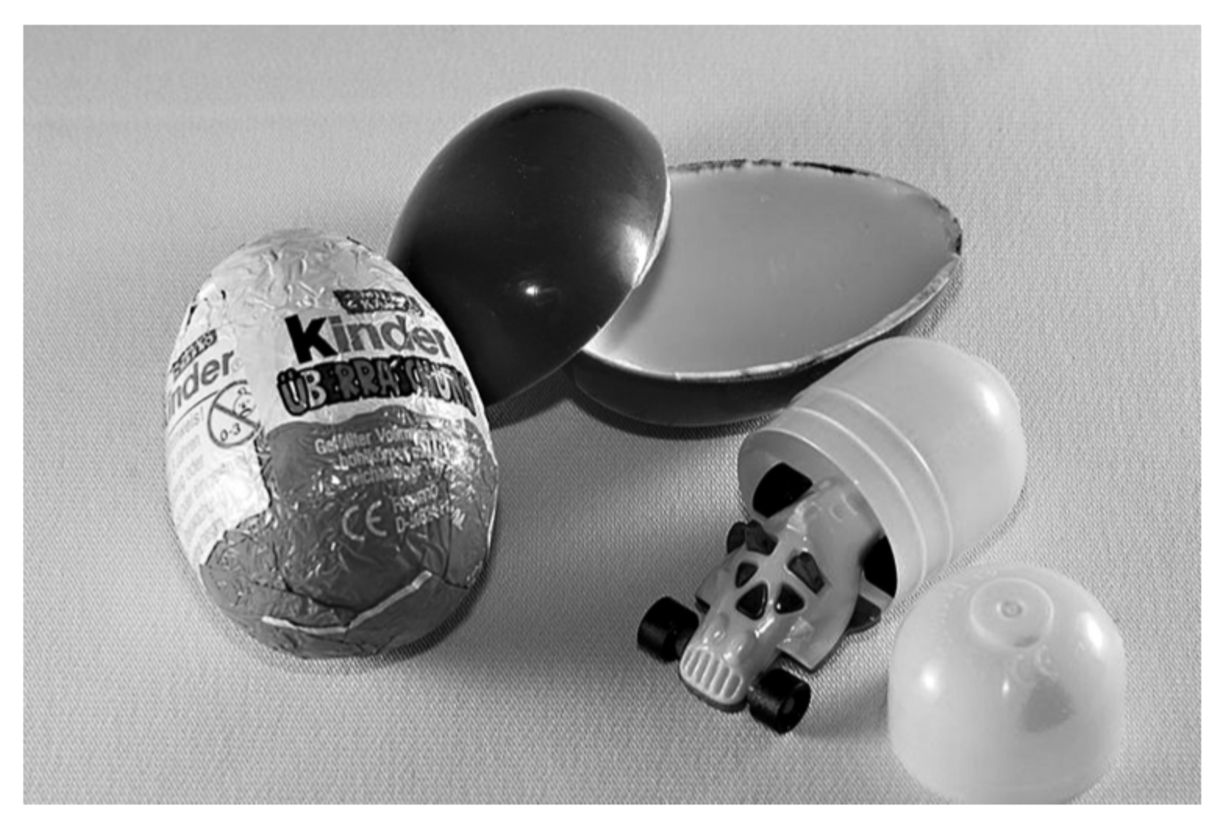
\includegraphics{../Bilder/Bild57-1.eps}}
\end{center}
\begin{scriptsize}\begin{singlespace}Bildquelle: https://de.wikipedia.org/wiki/Datei:Überraschungsei.jpg [01.06.2015] (Urheber: A. Kniesel, Lizenz: CC BY-SA 3.0)\end{singlespace}\end{scriptsize}

\subsection{Aufgabenstellung:}
\begin{enumerate}
	\item Bei der Qualitätskontrolle gelten Schokoladeneier, deren Masse um mehr als 0,5\,g vom Sollwert 20\,g abweichen, als Ausschuss. Bei einer Kontrolle wurden nach dem Zufallsprinzip 500 Schokoladeneier einer Produktionsserie ausgewählt und überprüft. Dabei wurden 15 als Ausschuss aussortiert.\leer
	
 Gib ein symmetrisches 90-\%-Konfidenzintervall für den relativen Anteil $p$ an Ausschusseiern in der gesamten Produktionsserie an!\leer

 Gib an, durch welche Maßnahme man die Breite des Konfidenzintervalls bei vorgegebenem Konfidenzniveau (Sicherheit) verringern kann!\leer

\item Der Hersteller überlegt, die gelbe Kapsel in Zukunft nur in Form eines Drehzylinders ohne aufgesetzte Halbkugeln zu produzieren. Das Volumen $V$ der Kapsel soll dabei unverändert bleiben, ebenso wie die Form des Schokoladeneies. Die Oberfläche $O(r)$ des angedachten Drehzylinders kann in Abhängigkeit vom Radius $r$ durch die Funktion $O$ mit der Gleichung $O(r)=2r²\pi+2\cdot V\cdot r^{-1}$ beschrieben werden. Der Radius $r$ darf dabei nur Werte im Bereich $(0\,cm; 1,9\,cm]$ annehmen, damit der Zylinder in das Schokoladenei passt.\leer

 Berechne die minimal mögliche Oberfläche der geplanten zylindrischen Kapsel!\leer

 Weise durch Differenzialrechnung nach, dass an der berechneten Stelle tatsächlich ein Minimum vorliegt!
						\end{enumerate}\leer
				
\antwort{
\begin{enumerate}
	\item \subsection{Lösungserwartung:} 
	
$h=0,03$

$0,03\,\pm\,1,645\cdot\sqrt{\frac{0,03\cdot(1-0,03)}{500}} \approx 0,03\,\pm\,0,013 \Rightarrow [0,017;0,043]$\leer

Mögliche Maßnahme:

Durch eine Erhöhung der Anzahl der kontrollierten Schokoladeneier auf mehr als 500 kann eine Verringerung der Breite des Konfidenzintervalls erreicht werden.
		
	\subsection{Lösungsschlüssel:}
	\begin{itemize}
		\item Ein Punkt für ein korrektes Intervall. Andere Schreibweisen des Ergebnisses (als Bruch oder Dezimalzahl) sind ebenfalls als richtig zu werten. 
		
		Toleranzintervall für den unteren Wert: $[0,017; 0,02]$ 
		
		Toleranzintervall für den oberen Wert: $[0,042; 0,05]$ 
		
		Die Aufgabe ist auch dann als richtig gelöst zu werten, wenn bei korrektem Ansatz das Ergebnis aufgrund eines Rechenfehlers nicht richtig ist. 
		\item Ein Punkt für eine (sinngemäß) korrekte Angabe der entsprechenden Änderung. Andere angeführte korrekte Maßnahmen sind ebenfalls als richtig zu werten.
	\end{itemize}
	
	\item \subsection{Lösungserwartung:}
			
			$O'(r)=4r\pi-72\cdot r^{-2}=4r\pi-\frac{72}{r²}$
	
	$4r\pi-\frac{72}{r²}=0$
	
	$r³=\frac{18}{\pi}$
	
	$r=\sqrt[3]{\frac{18}{\pi}} \Rightarrow r\approx 1,79$\,cm
	
	$O(1,79)\approx 60,4$\,cm$²$
	
	$O''(r)=4\pi+144\cdot r^{-3}=4\pi+\frac{144}{r³}$
	
	$O''(1,79)\approx 37,7>0$, daher liegt ein lokales Maximum vor.

	\subsection{Lösungsschlüssel:}
	
\begin{itemize}
	\item    Ein Punkt für eine korrekte Berechnung der minimalen Oberfläche, wobei die Einheit "`cm$²$"' nicht angeführt sein muss. 
	
	Toleranzintervall: $[60\,\text{cm}²; 61\,\text{cm}²] $ 
	
	Die Aufgabe ist auch dann als richtig gelöst zu werten, wenn bei korrektem Ansatz das Ergebnis aufgrund eines Rechenfehlers nicht richtig ist. 
	\item  Ein Punkt für einen korrekten Nachweis. Andere angeführte korrekte Nachweise sind ebenfalls als richtig zu werten. 
\end{itemize}

\end{enumerate}}
		\end{langesbeispiel}%
\hrule  \leer

\section{61 - MAT - WS 3.1, WS 3.2, WS 3.4,  - W�rfel mit unterschiedlichen Zahlen - Matura 2015/16 Haupttermin}

\begin{langesbeispiel} \item[0] %PUNKTE DES BEISPIELS
	
 Gegeben sind die Netze von drei fairen W�rfeln, deren Seitenfl�chen auf unterschiedliche Weise mit verschiedenen Zahlen beschriftet sind. (Ein W�rfel ist "`fair"', wenn die Wahrscheinlichkeit, nach einem Wurf nach oben zu zeigen, f�r alle Seitenfl�chen gleich gro� ist.)

\begin{center}
	\resizebox{0.9\linewidth}{!}{\psset{xunit=1.0cm,yunit=1.0cm,algebraic=true,dimen=middle,dotstyle=o,dotsize=4pt 0,linewidth=0.8pt,arrowsize=3pt 2,arrowinset=0.25}
\begin{pspicture*}(0.17804133915570747,4.040102465944372)(15.692206630376225,9.148214730906863)
\psline[linewidth=0.8pt](1.,7.)(1.,6.)
\psline[linewidth=0.8pt](1.,6.)(2.,6.)
\psline[linewidth=0.8pt](2.,6.)(2.,7.)
\psline[linewidth=0.8pt](2.,7.)(1.,7.)
\psline[linewidth=0.8pt](2.,6.)(3.,6.)
\psline[linewidth=0.8pt](3.,6.)(3.,5.)
\psline[linewidth=0.8pt](3.,5.)(4.,5.)
\psline[linewidth=0.8pt](4.,5.)(4.,6.)
\psline[linewidth=0.8pt](4.,6.)(5.,6.)
\psline[linewidth=0.8pt](5.,6.)(5.,7.)
\psline[linewidth=0.8pt](5.,7.)(4.,7.)
\psline[linewidth=0.8pt](4.,7.)(4.,8.)
\psline[linewidth=0.8pt](4.,8.)(3.,8.)
\psline[linewidth=0.8pt](3.,8.)(3.,7.)
\psline[linewidth=0.8pt](3.,7.)(2.,7.)
\psline[linewidth=0.8pt](3.,7.)(3.,6.)
\psline[linewidth=0.8pt](3.,7.)(4.,7.)
\psline[linewidth=0.8pt](3.,6.)(4.,6.)
\psline[linewidth=0.8pt](4.,7.)(4.,6.)
\psline[linewidth=0.8pt](5.94,6.97)(5.94,5.97)
\psline[linewidth=0.8pt](5.94,5.97)(6.94,5.97)
\psline[linewidth=0.8pt](6.94,5.97)(6.94,6.97)
\psline[linewidth=0.8pt](6.94,6.97)(5.94,6.97)
\psline[linewidth=0.8pt](6.94,5.97)(7.94,5.97)
\psline[linewidth=0.8pt](7.94,5.97)(7.94,4.97)
\psline[linewidth=0.8pt](7.94,4.97)(8.94,4.97)
\psline[linewidth=0.8pt](8.94,4.97)(8.94,5.97)
\psline[linewidth=0.8pt](8.94,5.97)(9.94,5.97)
\psline[linewidth=0.8pt](9.94,5.97)(9.94,6.97)
\psline[linewidth=0.8pt](9.94,6.97)(8.94,6.97)
\psline[linewidth=0.8pt](8.94,6.97)(8.94,7.97)
\psline[linewidth=0.8pt](8.94,7.97)(7.94,7.97)
\psline[linewidth=0.8pt](7.94,7.97)(7.94,6.97)
\psline[linewidth=0.8pt](7.94,6.97)(6.94,6.97)
\psline[linewidth=0.8pt](7.94,6.97)(7.94,5.97)
\psline[linewidth=0.8pt](7.94,6.97)(8.94,6.97)
\psline[linewidth=0.8pt](7.94,5.97)(8.94,5.97)
\psline[linewidth=0.8pt](8.94,6.97)(8.94,5.97)
\psline[linewidth=0.8pt](10.96,6.95)(10.96,5.95)
\psline[linewidth=0.8pt](10.96,5.95)(11.96,5.95)
\psline[linewidth=0.8pt](11.96,5.95)(11.96,6.95)
\psline[linewidth=0.8pt](11.96,6.95)(10.96,6.95)
\psline[linewidth=0.8pt](11.96,5.95)(12.96,5.95)
\psline[linewidth=0.8pt](12.96,5.95)(12.96,4.95)
\psline[linewidth=0.8pt](12.96,4.95)(13.96,4.95)
\psline[linewidth=0.8pt](13.96,4.95)(13.96,5.95)
\psline[linewidth=0.8pt](13.96,5.95)(14.96,5.95)
\psline[linewidth=0.8pt](14.96,5.95)(14.96,6.95)
\psline[linewidth=0.8pt](14.96,6.95)(13.96,6.95)
\psline[linewidth=0.8pt](13.96,6.95)(13.96,7.95)
\psline[linewidth=0.8pt](13.96,7.95)(12.96,7.95)
\psline[linewidth=0.8pt](12.96,7.95)(12.96,6.95)
\psline[linewidth=0.8pt](12.96,6.95)(11.96,6.95)
\psline[linewidth=0.8pt](12.96,6.95)(12.96,5.95)
\psline[linewidth=0.8pt](12.96,6.95)(13.96,6.95)
\psline[linewidth=0.8pt](12.96,5.95)(13.96,5.95)
\psline[linewidth=0.8pt](13.96,6.95)(13.96,5.95)
\rput[tl](1.4,6.6){1}
\rput[tl](2.4,6.6){2}
\rput[tl](3.4,6.6){1}
\rput[tl](4.4,6.6){2}
\rput[tl](3.4,7.6){3}
\rput[tl](3.4,5.6){3}
\rput[tl](6.3,6.6){-1}
\rput[tl](7.35,6.6){2}
\rput[tl](8.3,6.6){-1}
\rput[tl](9.35,6.6){2}
\rput[tl](8.35,7.6){5}
\rput[tl](8.35,5.6){5}
\rput[tl](11.4,6.6){0}
\rput[tl](12.4,6.6){0}
\rput[tl](13.4,6.6){6}
\rput[tl](13.4,5.6){6}
\rput[tl](13.4,7.6){0}
\rput[tl](14.4,6.6){6}
\rput[tl](2.6,8.665014922059061){W�rfel $A$}
\rput[tl](7.6,8.665014922059061){W�rfel $B$}
\rput[tl](12.6,8.665014922059061){W�rfel $C$}
\end{pspicture*}}
\end{center}



\subsection{Aufgabenstellung:}
\begin{enumerate}
	\item Herr Fischer wirft W�rfel $A$ zweimal. Die Zufallsvariable $X$ gibt die Summe der beiden geworfenen Zahlen an. Die Zufallsvariable $X$ kann die Werte 2,3,4,5 und 6 annehmen.
	
	Frau Fischer wirft die W�rfel $A$ und $B$. Die Zufallsvariable $Y$ gibt die Summe der beiden geworfenen Zahlen an.\leer
	
	\fbox{A} Gib f�r die Zufallsvariable $Y$ alle m�glichen Werte an!
	
	m�gliche Wert f�r $Y$: \rule{5cm}{0.3pt}
	
	Es gibt Werte der Zufallsvariablen, die bei Herrn Fischer wahrscheinlicher auftreten als bei Frau Fischer. Gib denjenigen Wert an, bei dem der Unterschied der beiden Wahrscheinlichkeiten am gr��ten ist, und berechne diesen Unterschied!
	
	\item Bei einem Spiel wird W�rfel $B$ dreimal geworfen. Der Einsatz des Spiels f�r eine Spielerin/einen Spieler betr�gt \EUR{2}. Die jeweilige Auszahlung ist von der Summe der drei geworfenen Zahlen abh�ngig und wird in der nachstehenden Tabelle teilweise angegeben
	
	\begin{center}
		\begin{tabular}{|c|c|}\hline
		\cellcolor[gray]{0.9}Summe der drei geworfenen Zahlen&\cellcolor[gray]{0.9}Auszahlung an die Spielerin/den Spieler\\ \hline
		positiv&0\\ \hline
		null&2\\ \hline
		negativ&?\\ \hline		
		\end{tabular}
	\end{center}

Eine Person spielt dieses Spiel f�nfmal. Berechne die Wahrscheinlichkeit, dass dabei genau zweimal die Summe der drei geworfenen Zahlen genau null ist!

 Berechne, welchen Betrag der Anbieter des Spiels f�r das W�rfeln einer negativen Summe h�chstens auszahlen darf, um langfristig mit keinem Verlust rechnen zu m�ssen! 

\item  Peter wirft den W�rfel $C$ 100-mal. Die Zufallsvariable $Z$ beschreibt die Anzahl der gew�rfelten Sechser.

 Berechne den Erwartungswert und die Standardabweichung von $Z$!

 Ermittle die Wahrscheinlichkeit, dass die Summe der geworfenen Zahlen gr��er als 350 ist!    
						\end{enumerate}\leer
				
\antwort{
\begin{enumerate}
	\item \subsection{L�sungserwartung:} 
	
m�gliche Werte f�r $Y$: $0, 1, 2, 3, 4, 5, 6, 7, 8$

Bei $Y$ hat jeder Wert die gleiche Wahrscheinlichkeit $\left(=\frac{1}{9}\right)$, bei $X$ hat 4 die gr��te Wahrscheinlichkeit $\left(=3\cdot\frac{1}{3}\cdot\frac{1}{3}=\frac{1}{3}\right)$. Der Unterschied ist bei 4 am gr��ten, er betr�gt $\frac{2}{9}$.

oder:

Die Wahrscheinlichkeit f�r 4 ist bei Herrn Fischer dreimal so gro� wie bei Frau Fischer.

	\subsection{L�sungsschl�ssel:}
	\begin{itemize}
		\item Ein Ausgleichspunkt f�r die vollst�ndige Angabe der korrekten Werte f�r $Y$. 
		\item Ein Punkt f�r die Angabe des gesuchten Wertes und einer korrekten Berechnung des Unterschieds.
	\end{itemize}
	
	\item \subsection{L�sungserwartung:}
			
	M�gliche Berechnung:
	
	Zufallsvariable $X$ = Anzahl der Spiele, bei denen die Summe der drei geworfenen Zahlen genau null ist.
	
	$P(\text{"`Summe der drei geworfenen Zahlen ist null"'})=p=\frac{1}{3}\cdot\frac{1}{3}\cdot\frac{1}{3}\cdot 3=\frac{1}{9}$
	
	Binomialverteilung mit den Parametern $n=5, k=2, p=\frac{1}{9}$
	
	$P(X=2)=\binom{5}{2}\cdot\left(\frac{1}{9}\right)�\cdot\left(\frac{8}{9}\right)�\approx 0,087 \Rightarrow$ Die gesuchte Wahrscheinlichkeit liegt bei ca. 8,7\,\%.
	
	M�gliche Berechnung:
	
	$x$ ... Auszahlung f�r das W�rfeln einer negativen Summe
	
	$2\cdot\frac{1}{9}+x\cdot\frac{1}{27}<2 \Rightarrow x<48$
	
	Die Auszahlung f�r das W�rfeln einer negativen Summe darf h�chstens \EUR{48} betragen, damit der Anbieter des Spiels langfristig mit keinem Verlust rechnen muss.

	\subsection{L�sungsschl�ssel:}
	
\begin{itemize}
	\item   Ein Punkt f�r die richtige L�sung. Andere Schreibweisen des Ergebnisses sind ebenfalls als richtig zu werten. 
	
	Toleranzintervall: $[0,08; 0,09]$ bzw. $[8\,\%; 9\,\%]$
	\item  Ein Punkt f�r die richtige L�sung, wobei die Einheit "`\EUR{ }"' nicht angegeben sein muss. Die Aufgabe ist auch dann als richtig gel�st zu werten, wenn bei korrektem Ansatz das Ergebnis aufgrund eines Rechenfehlers nicht richtig ist.

\end{itemize}

\item \subsection{L�sungserwartung:}
			
$n=100$ und $p=0,5$\leer

Erwartungswert: $E(Z)=50$

Standardabweichung: $\sqrt{V(Z)}=5$

M�gliche Berechnung (z.B. durch Approximation durch die Normalverteilung ohne Stetigkeitskorrektur):  

Die Summe ist gr��er als 350, wenn die Anzahl der Sechser mindestens 59 ist. Es ist m�glich, die (f�r die Anzahl der Sechser) zugrunde liegende Binomialverteilung mit $n=100$ und $p=0,5$ durch die Normalverteilung mit $\mu=50$ und $\sigma=5$ zu approximieren.

$P(Z\geq 59)\approx 0,036=36\,\%$

	\subsection{L�sungsschl�ssel:}
	
\begin{itemize}
	\item Ein Punkt f�r die Angabe der beiden korrekten Werte f�r den Erwartungswert und die Standardabweichung.
	\item Ein Punkt f�r die richtige L�sung, wobei Ergebnisse durch Berechnung mit Stetigkeitskorrektur oder exakt mittels Binomialverteilung ebenfalls als richtig zu werten sind. 
	
	Die Aufgabe ist auch dann als richtig gel�st zu werten, wenn bei korrektem Ansatz das Ergebnis aufgrund eines Rechenfehlers nicht richtig ist. 
	
	Toleranzintervall: $[0,035; 0,045]$ bzw. $[3,5\,\%; 4,5\,\%]$
\end{itemize}

\end{enumerate}}
		\end{langesbeispiel}%
\hrule  \leer

\section{64 - MAT - AG 4.1, AG 3.3, AG 3.4, WS 4.1 - Pong - Matura 2015/16 1. Nebentermin}

\begin{langesbeispiel} \item[0] %PUNKTE DES BEISPIELS
	
Das 1972 vom Unternehmen Atari veröffentlichte \textit{Pong} wurde zum ersten weltweit populären Videospiel. (Quelle: http://de.wikipedia.org/wiki/Pong)

Das Spielprinzip von \textit{Pong} ist wie folgt: Ein Punkt ("`Ball"') bewegt sich auf dem Bildschirm entlang geradliniger Bahnen hin und her. Jede/r der beiden Spieler/innen steuert einen senkrechten Strich ("`Schläger"'), den sie/er mit einem Drehknopf ("`Joystick"') nach oben und unten verschieben kann. 

Lässt man den Ball am Schläger vorbei, erhält die Gegnerin / der Gegner einen Punkt.

Das Spielfeld, in dem sich der Ball und die Schläger bewegen, hat eine Breite von 800 Pixeln und eine Höhe von 600 Pixeln (ein Pixel ist ein quadratischer Bildpunkt). Vereinfachend wird angenommen, dass der Ball als Pixel dargestellt wird. 

Wenn der Ball den oberen bzw. unteren Spielfeldrand oder einen Schläger berührt, dann wird er von dort reflektiert. Dabei gilt das Reflexionsgesetz; dieses besagt: $\alpha=\beta$ (vgl. die unten abgebildete Grafik).

Man kann sich das Spielfeld als Ebene mit Koordinatensystem vorstellen. Der Bildpunkt $(1|1)$ liegt dann in der linken unteren Ecke, der Bildpunkt $(800|600)$ in der rechten oberen Ecke.

Auf dem Schirm wird das Bild alle 0,02 Sekunden neu generiert. Der Geschwindigkeitsvektor $\vec{v}=\binom{v_x}{v_y}$ das Balls gibt an, um wie viele Pixel sich der Ball von einem Bildaufbau zum nächsten in horizontaler Richtung $\left(v_x\right)$ und in vertikaler Richtung $\left(v_y\right)$ weiterbewegt hat.

\begin{center}
	\resizebox{0.5\linewidth}{!}{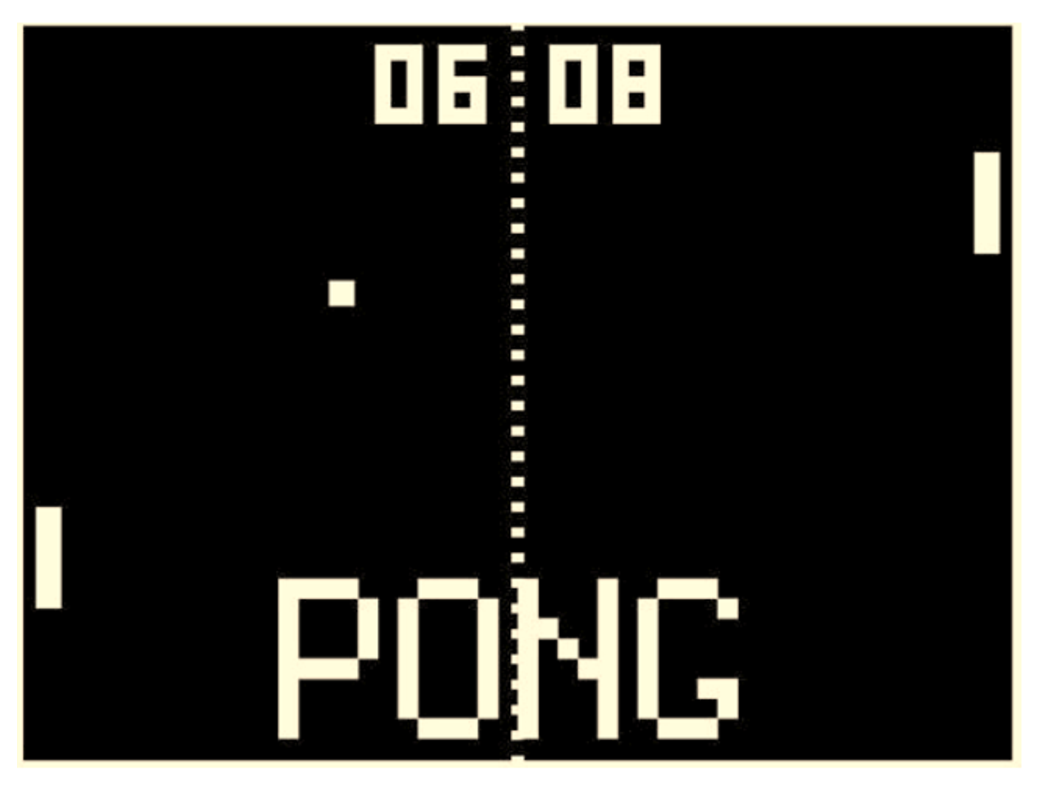
\includegraphics{../_database/Bilder/Bild64-1.eps}}
\end{center}
\begin{scriptsize} Bildquelle: http://www.overclockers.at/games\_forum/euer-erstes-computerspiel\_237146/page\_2 [15.10.2015]. \end{scriptsize}

\begin{center}
	\resizebox{0.5\linewidth}{!}{\newrgbcolor{qqwuqq}{0. 0.39215686274509803 0.}
\psset{xunit=1.0cm,yunit=1.0cm,algebraic=true,dimen=middle,dotstyle=o,dotsize=4pt 0,linewidth=0.8pt,arrowsize=3pt 2,arrowinset=0.25}
\begin{pspicture*}(0.66,5.447272727272732)(8.9,8.537922077922087)
\multips(0,5)(0,1.0){4}{\psline[linestyle=dashed,linecap=1,dash=1.5pt 1.5pt,linewidth=0.4pt,linecolor=lightgray]{c-c}(0.66,0)(8.9,0)}
\multips(0,0)(1.0,0){9}{\psline[linestyle=dashed,linecap=1,dash=1.5pt 1.5pt,linewidth=0.4pt,linecolor=lightgray]{c-c}(0,5.447272727272732)(0,8.537922077922087)}
\psaxes[labelFontSize=\scriptstyle,xAxis=true,yAxis=true,Dx=1.,Dy=1.,ticksize=-2pt 0,subticks=2]{->}(0,0)(0.66,5.447272727272732)(8.9,8.537922077922087)
\psplot[linewidth=0.8pt]{0.66}{8.9}{(--56.-0.*x)/7.}
\psline[linewidth=0.8pt]{->}(5.,8.)(8.,6.)
\psline[linewidth=0.8pt]{->}(2.,6.)(5.,8.)
\pscustom[linewidth=0.8pt,linecolor=qqwuqq,fillcolor=qqwuqq,fillstyle=solid,opacity=0.1]{
\parametricplot{-0.5880026035475675}{0.0}{1.4*cos(t)+5.|1.4*sin(t)+8.}
\lineto(5.,8.)\closepath}
\pscustom[linewidth=0.8pt,linecolor=qqwuqq,fillcolor=qqwuqq,fillstyle=solid,opacity=0.1]{
\parametricplot{3.141592653589793}{3.7295952571373605}{1.4*cos(t)+5.|1.4*sin(t)+8.}
\lineto(5.,8.)\closepath}
\rput[bl](5.8,7.5){\qqwuqq{$\beta$}}
\rput[bl](3.9,7.58){\qqwuqq{$\alpha$}}
\end{pspicture*}}
\end{center}

\subsection{Aufgabenstellung:}
\begin{enumerate}
	\item In einer konkreten Spielsituation hat der Ball beim Aufprall auf den oberen Spielfeldrand einen Geschwindigkeitsvektor von $\vec{v}=\binom{4}{7}$ Pixeln pro Bildaufbau.
	
	\fbox{A} Gib denjenigen Winkel $\alpha$ an, unter dem der Ball auf den Spielfeldrand trifft!
	
	$\alpha$= \rule{5cm}{0.3pt}
	
	Die Komponenten des Geschwindigkeitsvektors sind immer ganzzahlig. Nehmen Sie an, dass die Summe der Beträge der Komponenten nicht größer als 20 sein darf.
	
	Der Ball wird am oberen Spielfeldrand unter dem Winkel $\beta$ reflektiert. Welchen kleinstmöglichen Wert $\beta_\text{min}$ kann unter diesen Voraussetzungen der Winkel $\beta$ annehmen? Gib $\beta_\text{min}$ an!
	
	$\beta_\text{min}$= \rule{5cm}{0.3pt}
	
	\item In einem anderen Spielverlauf befindet sich der Ball im Punkt $(401|301)$ und sein Geschwindigkeitsvektor ist dabei $\vec{v}=\binom{2}{-3}$ Pixel pro Bildaufbau.
	
	Gib an, wie viele \textit{Sekunden} es dauert, bis der Ball am unteren Spielfeldrand reflektiert wird.
	
	Nach dieser Reflexion bewegt sich der Ball entlang einer Geraden bis zum nächsten Auftreffen auf den Schläger oder den Spielfeldrand.
	
 Gib eine Parameterdarstellung dieser Geraden an! 

\item Zwei Kinder, Nicola und Florian, spielen über einen längeren Zeitraum oft gegeneinander \textit{Pong}. Von 45 Spielen gewinnt Nicola 31-mal, Florian gewinnt 14-mal.
 
		Gib auf Basis dieser Information ein symmetrisches $95-\%-$Konfidenzintervall für Nicolas Gewinnwahrscheinlichkeit an!
		
		Erkläre, wieso es nicht sinnvoll ist, ein 100-\%-Konfidenzintervall zu bestimmen!
\end{enumerate}
\antwort{
\begin{enumerate}
	\item \subsection{Lösungserwartung:} 
	
$\tan(\alpha)=\frac{7}{4}=1,74$

$\alpha\approx 60,26^\circ$

Unter diesen Bedingungen lautet der Geschwindigkeitsvektor $\vec{v}= \binom{\pm\,19}{\pm\,1}$ Pixel pro Bildaufbau. Für den Winkel $\beta_\text{min}$ gibt das in jedem Fall:

 $\tan(\beta_\text{min})=\frac{1}{19}$

 $\beta_\text{min}\approx 3,01^\circ$

	\subsection{Lösungsschlüssel:}
	\begin{itemize}
		\item Ein Ausgleichspunkt für die richtige Lösung, wobei die Einheit "`Grad"' nicht angegeben sein muss. Eine korrekte Angabe der Lösung in einer anderen Einheit ist ebenfalls als richtig zu werten. 
		
		Toleranzintervall: $[6011^\circ; 60,3^\circ]$
		\item Ein Punkt für die richtige Lösung, wobei die Einheit "`Grad"' nicht angegeben sein muss. Eine korrekte Angabe der Lösung in einer anderen Einheit ist ebenfalls als richtig zu werten. 
		
		Toleranzintervall: $[3^\circ; 3,02^\circ]$
	\end{itemize}
	
	\item \subsection{Lösungserwartung:}
			
	$301-3n=1 \Rightarrow n=100$
	
	$100\cdot 0,02=2$
	
	Es dauert zwei Sekunden, bis der Ball am unteren Spielfeldrand reflektiert wird.\leer
	
	$g: X=\binom{601}{1}+s\cdot\binom{2}{3}$

	\subsection{Lösungsschlüssel:}
	
\begin{itemize}
	\item Ein Punkt für die richtige Lösung. 
	
	Toleranzintervall: $[2\,\text{s}; 2,02\,\text{s}]$
	\item Ein Punkt für eine korrekte Parameterdarstellung bzw. Gleichung der Geraden. Äquivalente Parameterdarstellungen bzw. Gleichungen sind als richtig zu werten. 
\end{itemize}

\item \subsection{Lösungserwartung:}
			
$n=45, h=\frac{31}{45}$

$\frac{31}{45}\,\pm\,1,96\cdot\sqrt{\frac{\frac{31}{45}\cdot\frac{14}{45}}{45}}\approx 0,689\,\pm\,0,135 \Rightarrow [0,554;0,824]$\leer

Mögliche Erklärungen:

Es ist nicht sinnvoll, ein 100-\%-Konfidenzintervall zu bilden, da die Intervallgrenzen dann 0\,\% bis 100\.\% wären, man hätte also keinen Informationsgewinn. 

 oder:  

 Ein 100-\%-Konfidenzintervall erstreckt sich über den gesamten Definitionsbereich.
	\subsection{Lösungsschlüssel:}
	
\begin{itemize}
	\item Ein Punkt für ein korrektes Intervall. Andere Schreibweisen des Ergebnisses (als Bruch oder in Prozent) sind ebenfalls als richtig zu werten. 
	
	Toleranzintervall für den unteren Wert: $[0,54; 0,56]$ 
	
	Toleranzintervall für den oberen Wert: $[0,81; 0,83]$ 
	
	Die Aufgabe ist auch dann als richtig gelöst zu werten, wenn bei korrektem Ansatz das Ergebnis aufgrund eines Rechenfehlers nicht richtig ist. 
	\item Ein Punkt für eine (sinngemäß) korrekte Erklärung.
\end{itemize}
\end{enumerate}}
		\end{langesbeispiel}%
\hrule  \leer

\section{65 - MAT - WS 2.1, WS 3.4, WS 2.3 - Roulette - Matura 2015/16 1. Nebentermin}

\begin{langesbeispiel} \item[0] %PUNKTE DES BEISPIELS
	
Beim Gl�cksspiel \textit{Roulette} versucht man, diejenige Zahl bzw. Gruppe von Zahlen zu erraten, die durch den Wurf einer Kugel in die Roulettemaschine bestimmt wird. 

Beim \textit{franz�sischen Roulette} besteht die Roulettemaschine aus einer in eine Sch�ssel eingelassenen, drehbaren Scheibe mit 36 abwechselnd roten und schwarzen Nummernf�chern sowie einem 37., gr�n gekennzeichneten Fach f�r die Null (vgl. Abbildung 1). Die Roulettescheibe wird in Bewegung gesetzt und die Kugel wird gegen die Drehrichtung in die Roulettemaschine geworfen. Dabei wird kein Nummernfach bevorzugt und es gibt keine M�glichkeit, das Ergebnis (etwa durch "`geschicktes"' Werfen) zu beeinflussen. 

Ziel ist es, in jedem einzelnen Spiel im Vorhinein zu erraten, in welchem Nummernfach die Kugel zu liegen kommen wird. 

Auf dem Spielfeld (vgl. Abbildung 2) werden die Spieleins�tze (Jetons) platziert. Beispielsweise sind die Felder mit der "`1"' und der "`7"' rot ("`rouge"'), die Felder mit der "`4"' und der "`6"' schwarz ("`noir"').

\meinlr{\resizebox{1\linewidth}{!}{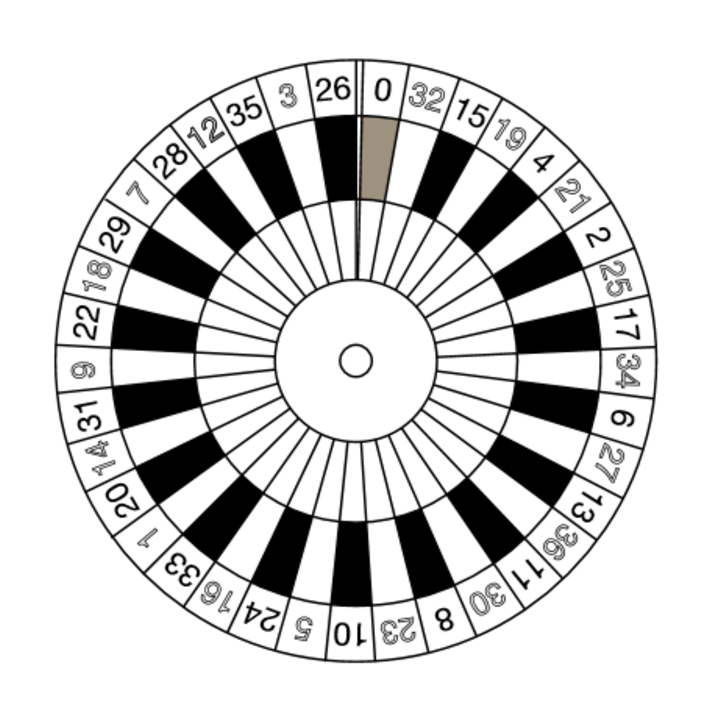
\includegraphics{../Bilder/Bild65-1.eps}}

Abbildung 1

\begin{scriptsize}\begin{singlespace}Quelle:http://www.rouletteplay.com/images/\\
software\_logos\_small/european-roulette-wheel.gif [23.03.2016]\end{singlespace}\end{scriptsize}}{\resizebox{0.8\linewidth}{!}{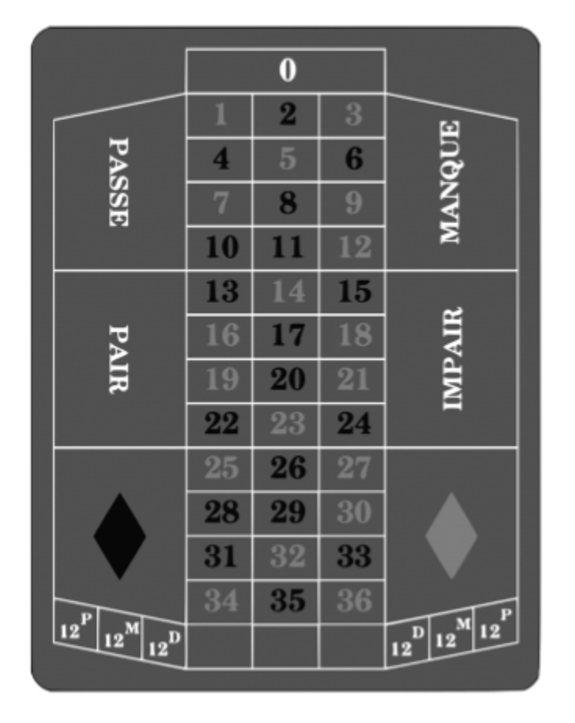
\includegraphics{../Bilder/Bild65-2.eps}}

Abbildung 2

\begin{scriptsize}\begin{singlespace}Quelle:http://commons.wikimedia.org/wiki/\\
File:Roulette\_frz.png [23.03.2016]\end{singlespace}\end{scriptsize}}
 

\subsection{Aufgabenstellung:}
\begin{enumerate}
	\item Jemand argumentiert: "`Wenn die Kugel bei f�nf Spielen hintereinander jedes Mal auf ein rotes Feld gefallen ist, f�llt die Kugel beim 6. Spiel mit h�herer Wahrscheinlichkeit auf ein schwarzes Feld als auf ein rotes, da bei einer l�ngeren Spielserie dieselben H�ufigkeiten f�r 'Rouge' und 'Noir' zu erwarten sind."' Gib an, ob diese Argumentation richtig oder falsch ist, und begr�nde deine Entscheidung!\leer
	
	An einem Roulettetisch werden an einem Abend 100 Spiele gespielt.
	
	\fbox{A} Berechne die Wahrscheinlichkeit, dass die Kugel dabei h�chstens 40-mal in ein rotes Nummernfach f�llt!\leer
	
	\item In der folgenden Tabelle sind einige Wettm�glichkeiten sowie die jeweiligen Gewinnquoten angef�hrt:\leer
	
	\begin{tabular}{|l|c|}\hline
	\cellcolor[gray]{0.9}Wettart&\cellcolor[gray]{0.9}Gewinnquote\\ \hline
	Rouge: Die Kugel f�llt in ein rotes Nummernfach.&1:1\\ \hline
	Noir: Die Kugel f�llt in ein schwarzes Nummernfach.&1:1\\ \hline
	$12^\text{P}$: erstes Dutzend (Zahlen 1 bis 12)&2:1\\ \hline
	$12^\text{M}$: mittleres Dutzend (Zahlen 13 bis 24)&2:1\\ \hline
	$12^\text{D}$: letztes Dutzend (Zahlen 25 bis 36)&2:1\\ \hline
	Plein: Man setzt auf eine der 37 Zahlen&35:1\\ \hline
	\multicolumn{1}{|p{10cm}|}{Cheval: Man setzt auf zwei auf dem Spielfeld horizontal oder vertikal benachbarte Zahlen, z.B. 2 und 5 oder 8 und 9.}&17:1\\ \hline	
	\end{tabular}\leer
	
 Eine Gewinnquote von $2:1$ bedeutet beispielsweise, dass im Falle eines Gewinns der Einsatz und zus�tzlich das Doppelte des Einsatzes ausbezahlt wird. Im Falle eines Verlustes verliert man den Einsatz.

 Als Bankvorteil bezeichnet man bei Gl�cksspielen den erwarteten Verlust der Spielerin/des Spielers bezogen auf ihren/seinen Einsatz.

Eine Spielerin setzt \EUR{10} auf $12^\text{M}$. 

Berechne den Bankvorteil in Prozent des Einsatzes! 
 
Gib an, ob der in Prozent angegebene Bankvorteil gr��er wird, kleiner wird oder gleich bleibt, wenn die Spielerin/der Spieler bei einem Einsatz von \EUR{$a$} eine Cheval-Variante w�hlt!  

Begr�nde deine Entscheidung!


	
\end{enumerate}
\antwort{
\begin{enumerate}
	\item \subsection{L�sungserwartung:} 
	
Die Argumentation ist falsch. Da die einzelnen Spiele unabh�ngig voneinander sind, gilt auch f�r das sechste Spiel (unabh�ngig von den vorherigen Spielausg�ngen):

$P(\text{"`Rouge"'})=P(\text{"`Noir"'})=\frac{18}{37}$\leer

M�gliche Berechnung (z.B. durch Approximation durch die Normalverteilung ohne Stetigkeitskorrektur):  

Die binomialverteilte Zufallsvariable $X$ beschreibt, wie oft die Kugel in ein rotes Nummernfach f�llt.

$n=100, p=\frac{18}{37}$

$P(X\leq 40)\approx 0,0418$ 

	\subsection{L�sungsschl�ssel:}
	\begin{itemize}
		\item  Ein Punkt f�r die Angabe, dass die Argumentation nicht richtig ist, und f�r eine (sinngem��) korrekte Begr�ndung.
		\item  Ein Ausgleichspunkt f�r die richtige L�sung, wobei Ergebnisse durch Berechnung mit Stetigkeitskorrektur oder exakt mittels Binomialverteilung ebenfalls als richtig zu werten sind. Andere Schreibweisen des Ergebnisses (in Prozent) sind ebenfalls als richtig zu werten. 
		
		Toleranzintervall: $[0,03; 0,06]$  
		
		Die Aufgabe ist auch dann als richtig gel�st zu werten, wenn bei korrektem Ansatz das Ergebnis aufgrund eines Rechenfehlers nicht richtig ist. 
	\end{itemize}
	
	\item \subsection{L�sungserwartung:}
			
	M�gliche Berechnung:
	
	Bei $12^\text{M}$ erh�lt die Spielerin bei einem Einsatz von \EUR{10} mit der Wahrscheinlichkeit $\frac{12}{37}$ einen Gewinn von \EUR{20}.
	
	$\frac{12}{37}\cdot 20-\frac{25}{37}\cdot 10\approx -0,27$
	
	D.h., der erwartete Verlust betr�gt ca. \EUR{0,27}.
	
	Bankvorteil: \EUR{0,27} bzw. 2,7\,\% des Einsatzes\leer
	
	Cheval bei einem Einsatz von \EUR{$a$}:
	
	erwarteter Gewinn: $\frac{2}{37}\cdot 17\cdot a-\frac{35}{37}\cdot a=-\frac{1}{37}\cdot a\approx -0,027\cdot a$
	
	Der Bankvorteil bleibt mit ca. 2,7\,\% des Einsatzes gleich.
	
	\subsection{L�sungsschl�ssel:}
	
\begin{itemize}
	\item Ein Punkt f�r die richtige L�sung, wobei diese sowohl in Prozentangabe als auch als Geldbetrag als richtig zu werten ist. 
	
	Toleranzintervall: [\EUR{0,27}; \EUR{0,30}] bzw. $[2,7\,\%; 3\,\%]$ 
	\item Ein Punkt f�r die Angabe, dass der Bankvorteil gleich bleibt, und f�r eine (sinngem��) korrekte Begr�ndung.  
\end{itemize}

\end{enumerate}}
		\end{langesbeispiel}%
\hrule  \leer

\section{68 - MAT - WS 1.2, WS 1.3, WS 1.4 - Nettomonatseinkommen - Matura 2015/16 2. Nebentermin}

\begin{langesbeispiel} \item[0] %PUNKTE DES BEISPIELS
	
Das Nettomonatseinkommen erwerbstätiger Personen hängt von sozioökonomischen Faktoren wie Alter, Staatsangehörigkeit, Schulbildung, Beschäftigungsausmaß und beruflicher Stellung ab. Die nachstehende Tabelle zeigt Daten zu den Nettomonatseinkommen unselbständig Erwerbstätiger in Österreich im Jahresdurchschnitt 2010 in Abhängigkeit von sozioökonomischen Faktoren. Alle folgenden Aufgabenstellungen beziehen sich auf diese Daten des Jahres 2010.\leer

\begin{tiny}
\begin{tabular}{|C{1.4cm}|C{1.4cm}|C{1.4cm}|C{1.4cm}|C{1.4cm}|C{1.4cm}|C{1.4cm}|C{1.4cm}|}\hline
\multirow{3}{1.1cm}{Merkmale}&\multicolumn{1}{C{1.1cm}|}{\multirow{2}{1.1cm}{unselbst- ständig Erwerbstätige}}&\multicolumn{1}{C{1.1cm}|}{\multirow{2}{1.1cm}{arithme- tisches Mittel}}&\multirow{2}{1.4cm}{\centering$10\,\%$}&\multicolumn{3}{c|}{Quartile}&\multirow{2}{1.1cm}{\centering$90\,\%$}\\ \cline{5-7}
&&&&$25\,\%$&$50\,\%$ (Median)&$75\,\%$& \\ \cline{2-8}
&\multicolumn{1}{C{1.4cm}|}{\mbox{in 1000} \mbox{Personen}}&in Euro&\multicolumn{5}{c|}{verdienen weniger als oder gleich viel wie ... Euro} \\ \hline
\end{tabular}

\begin{tabular}{p{1.4cm}C{1.4cm}C{1.4cm}C{1.4cm}C{1.4cm}C{1.4cm}C{1.4cm}C{1.4cm}}
\textbf{Insgesamt}&3\,407,9&1\,872,7&665,0&1\,188,0&1\,707&2\,303,0&3\,122,0\\\leer

\textbf{Alter}&&&&&&&\\
15-19 Jahre&173,5&799,4&399,0&531,0&730,0&1\,020,0&1\,315,0\\
20-29 Jahre&705,1&1\,487,0&598,0&1\,114,0&1\,506,0&1\,843,0&2\,175,0\\
30-39 Jahre&803,1&1\,885,7&770,0&1\,252,0&1\,778,0&2\,306,0&2\,997,0\\
40-49 Jahre&1\,020,4&2\,086,1&863,0&1\,338,0&1\,892,0&2\,556,0&3\,442,0\\
50-59 Jahre&632,8&2\,205,0&893,0&1\,394,0&1\,977,0&2\,779,0&3\,710,0\\
60+ Jahre&73,0&2\,144,7&258,0&420,0&1\,681,0&3\,254,0&4\,808,0\\
&&&&&&&\\
\multicolumn{3}{l}{\textbf{Höchste abgeschlossene Schulbildung}}&&&&&\\
Pflichtschule&523,4&1\,183,0&439&677,0&1\,104,0&1\,564,0&1\,985,0\\
Lehre&1\,385,2&1\,789,3&833,0&1\,303,0&1\,724,0&2\,143,0&2\,707,0\\
BMS&454,4&1\,777,1&733,0&1\,199,0&1\,677,0&2\,231,0&2\,824,0\\
Höhere Schule&557,2&2\,061,6&590,0&1\,218,0&1\,824,0&2\,624,0&3\,678,0\\
Universität&487,7&2\,723,4&1\,157,0&1\,758,0&2\,480,0&3\,376,0&4\,567,0\\
&&&&&&&\\
\multicolumn{3}{l}{\textbf{Berufliche Stellung}}&&&&&\\
Lehrlinge&134,2&775,3&466,0&551,0&705,0&930,0&1\,167,0\\
Angestellte(r)&1\,800,3&2\,018,1&705,0&1\,222,0&1\,771,0&2\,489,0&3\,550,0\\
Arbeiter(in)&1\,030,9&1\,539,3&627,0&1\,135,0&1\,554,0&1\,922,0&2\,274,0\\
Beamte und Vertragsbedienstete&442,5&2\,391,4&1\,377,0&1\,800,0&2\,295,0&2\,848,0&3\,492,0
\end{tabular}
\begin{singlespace}Datenquelle: Statistik Austria (Hrsg.) (2012). Arbeitsmarktstatistik. Jahresergebnisse 2011. Mikrozensus-Arbeitskräfteerhebung. 
 Wien: Statistik Austria. S. 81 (adaptiert)\end{singlespace}
\end{tiny}

\subsection{Aufgabenstellung:}
\begin{enumerate}
	\item Zeichne in der nachstehenden Grafik ein Diagramm, das die Medianeinkommen der 20- bis 59-Jährigen darstellt! Verwende dafür die auf die Hunderterstelle gerundeten Medianeinkommen.
	
	\begin{center}
		\resizebox{0.8\linewidth}{!}{\newrgbcolor{uququq}{0.25098039215686274 0.25098039215686274 0.25098039215686274}
\psset{xunit=2.0cm,yunit=0.0001cm,algebraic=true,dimen=middle,dotstyle=o,dotsize=4pt 0,linewidth=0.8pt,arrowsize=3pt 2,arrowinset=0.25}
\begin{pspicture*}(-0.7735499280941546,-6798.3471820682125)(4.846644372997255,67316.8397144404)
\multips(0,0)(0,10000.0){8}{\psline[linestyle=dashed,linecap=1,dash=1.5pt 1.5pt,linewidth=0.4pt,linecolor=lightgray]{c-c}(0,0)(4.846644372997255,0)}
\multips(0,0)(1,0){6}{\psline[linestyle=dashed,linecap=1,dash=1.5pt 1.5pt,linewidth=0.4pt,linecolor=lightgray]{c-c}(0,0)(0,67316.8397144404)}
\psaxes[labelFontSize=\scriptstyle,xAxis=true,yAxis=true,labels=none,Dx=1.,Dy=10000.,ticksize=-2pt 0,subticks=2]{->}(0,0)(0.,0.)(4.846644372997255,67316.8397144404)
\begin{scriptsize}
\rput[tl](4.438293735441856,-1568.8084472780674){Alter}
\rput[tl](0.25,-1000){$20-29$}
\rput[tl](1.25,-1000){$30-39$}
\rput[tl](2.25,-1000){$40-49$}
\rput[tl](3.25,-1000){$50-59$}
\rput[tl](-0.4,1000){$1\,000$}
\rput[tl](-0.4,11000){$1\,200$}
\rput[tl](-0.4,21000){$1\,400$}
\rput[tl](-0.4,31000){$1\,600$}
\rput[tl](-0.4,41000){$1\,800$}
\rput[tl](-0.4,51000){$2\,000$}
\rput[tl](-0.4,61000){$2\,200$}
\rput[tl](0.18285024933822672,66054.53726121518){Euro}
\end{scriptsize}
\end{pspicture*}}
	\end{center}
	
	Ist es anhand der Daten in der gegebenen Tabelle möglich, die Nettomonatseinkommen der 20- bis 29-Jährigen und der 30- bis 39-Jährigen in Boxplots (Kastenschaubildern) gegenüberzustellen? Begründe deine Antwort!
	
	\item Jemand hat das arithmetische Mittel aller Nettomonatseinkommen anhand der arithmetischen Mittel der sechs Altersklassen folgendermaßen berechnet:
	
	$\frac{799,4+1\,487,0+1\,885,7+2\,086,1+2\,205,0+2\,144,7}{6}\approx 1\,768,0$
	
	In der gegebenen Tabelle ist allerdings für das arithmetische Mittel aller Einkommen der Wert 1 872,7 angegeben. 
	
	Begründe, warum die oben angeführte Rechnung nicht das richtige Ergebnis liefert, und gib den richtigen Ansatz für die Berechnung an! \leer
	
	Bei der Altersklasse 60+ ist das arithmetische Mittel der Nettomonatseinkommen deutlich (um fast \EUR{500}) größer als das Medianeinkommen dieser Altersklasse. Gib eine daraus ableitbare Schlussfolgerung im Hinblick auf sehr niedrige bzw. sehr hohe Nettomonatseinkommen in dieser Altersklasse an!
	
	\item \fbox{A} Gib die Werte des 1. und des 3. Quartils der Nettomonatseinkommen der unselbstständig Erwerbstätigen mit Pflichtschulabschluss als höchste abgeschlossene Schulbildung an!
	
	1. Quartil: \rule{3cm}{0.3pt}
	
	3. Quartil: \rule{3cm}{0.3pt}\leer
	
	Der Interquartilsabstand ist die Differenz von 3. und 1. Quartil. 
	
	Ein Experte behauptet: "`Mit zunehmender höchster abgeschlossener Schulbildung, die über einen Pflichtschulabschluss hinausgeht, nimmt auch der Interquartilsabstand der Nettomonatseinkommen zu."' 
	
	Verifiziere oder widerlege diese Behauptung und verwende dazu die Daten in der gegebenen Tabelle!
 
	\item Die Daten in der gegebenen Tabelle zeigen, dass ungefähr 53\,\% der unselbständig Erwerbstätigen Angestellte und ungefähr 30\,\% Arbeiter/innen sind. 
	
	In einem Kommentar zum Arbeitsmarktbericht ist zu lesen: "`Der relative Anteil der Angestellten ist um ungefähr 23\,\% höher als der relative Anteil der Arbeiter/innen."' Ist diese Aussage richtig? Begründe deine Antwort! 
	
	Überprüfe folgende Aussagen über Nettomonatseinkommen anhand der Daten in der gegebenen Tabelle! Kreuze die beiden zutreffenden Aussagen an!\leer
	
	\multiplechoice[5]{  %Anzahl der Antwortmoeglichkeiten, Standard: 5
					L1={Angestellte verdienen im Durchschnitt um über \EUR{500} mehr als Arbeiter/innen.},   %1. Antwortmoeglichkeit 
					L2={Höchstens ein Viertel der Arbeiter/innen verdient mehr als \EUR{1.922}. },   %2. Antwortmoeglichkeit
					L3={Die Spannweite des Nettomonatseinkommens kann anhand der Daten in der Tabelle nicht exakt angegeben werden.},   %3. Antwortmoeglichkeit
					L4={Drei Viertel der Lehrlinge verdienen mindestens \EUR{930}.},   %4. Antwortmoeglichkeit
					L5={Genau die Hälfte der Beamten und Vertragsbediensteten verdient exakt \EUR{1.800}.},	 %5. Antwortmoeglichkeit
					L6={},	 %6. Antwortmoeglichkeit
					L7={},	 %7. Antwortmoeglichkeit
					L8={},	 %8. Antwortmoeglichkeit
					L9={},	 %9. Antwortmoeglichkeit
					%% LOESUNG: %%
					A1=2,  % 1. Antwort
					A2=3,	 % 2. Antwort
					A3=0,  % 3. Antwort
					A4=0,  % 4. Antwort
					A5=0,  % 5. Antwort
					}

\end{enumerate}

\antwort{
\begin{enumerate}
	\item \subsection{Lösungserwartung:} 

Mögliches Diagramm:

\begin{center}
		\resizebox{0.8\linewidth}{!}{\newrgbcolor{uququq}{0.25098039215686274 0.25098039215686274 0.25098039215686274}
\psset{xunit=2.0cm,yunit=0.0001cm,algebraic=true,dimen=middle,dotstyle=o,dotsize=4pt 0,linewidth=0.8pt,arrowsize=3pt 2,arrowinset=0.25}
\begin{pspicture*}(-0.7735499280941546,-6798.3471820682125)(4.846644372997255,67316.8397144404)
\multips(0,0)(0,10000.0){8}{\psline[linestyle=dashed,linecap=1,dash=1.5pt 1.5pt,linewidth=0.4pt,linecolor=lightgray]{c-c}(0,0)(4.846644372997255,0)}
\multips(0,0)(1,0){6}{\psline[linestyle=dashed,linecap=1,dash=1.5pt 1.5pt,linewidth=0.4pt,linecolor=lightgray]{c-c}(0,0)(0,67316.8397144404)}
\psaxes[labelFontSize=\scriptstyle,xAxis=true,yAxis=true,labels=none,Dx=1.,Dy=10000.,ticksize=-2pt 0,subticks=2]{->}(0,0)(0.,0.)(4.846644372997255,67316.8397144404)
\pspolygon[linewidth=0.8pt,linecolor=uququq,fillcolor=uququq,fillstyle=solid,opacity=0.69](0.,0.)(0.,25000.)(1.,25000.)(1.,0.)
\pspolygon[linewidth=0.8pt,linecolor=uququq,fillcolor=uququq,fillstyle=solid,opacity=0.69](1.,0.)(1.,40000.)(2.,40000.)(2.,0.)
\pspolygon[linewidth=0.8pt,linecolor=uququq,fillcolor=uququq,fillstyle=solid,opacity=0.69](2.,0.)(2.,45000.)(3.,45000.)(3.,0.)
\pspolygon[linewidth=0.8pt,linecolor=uququq,fillcolor=uququq,fillstyle=solid,opacity=0.69](3.,0.)(3.,50000.)(4.,50000.)(4.,0.)
\begin{scriptsize}
\rput[tl](4.438293735441856,-1568.8084472780674){Alter}
\rput[tl](0.25,-1000){$20-29$}
\rput[tl](1.25,-1000){$30-39$}
\rput[tl](2.25,-1000){$40-49$}
\rput[tl](3.25,-1000){$50-59$}
\rput[tl](-0.4,1000){$1\,000$}
\rput[tl](-0.4,11000){$1\,200$}
\rput[tl](-0.4,21000){$1\,400$}
\rput[tl](-0.4,31000){$1\,600$}
\rput[tl](-0.4,41000){$1\,800$}
\rput[tl](-0.4,51000){$2\,000$}
\rput[tl](-0.4,61000){$2\,200$}
\rput[tl](0.18285024933822672,66054.53726121518){Euro}
\end{scriptsize}
\end{pspicture*}}
	\end{center}
 
Die Gegenüberstellung der Nettomonatseinkommen in Boxplots (Kastenschaubildern) ist anhand der gegebenen Daten nicht möglich, da die niedrigsten und die höchsten Nettomonatseinkommen (Minimum und Maximum) in der Tabelle nicht angegeben sind.

	\subsection{Lösungsschlüssel:}
	\begin{itemize}
		\item Ein Punkt für ein korrektes Diagramm.
		\item Ein Punkt für eine (sinngemäß) richtige Begründung. 
	\end{itemize}
	
	\item \subsection{Lösungserwartung:}
			
Mögliche Begründung:

Die angeführte Rechnung ist falsch, da die Anzahl der Erwerbstätigen in den einzelnen Altersklassen nicht berücksichtigt ist.

Ein richtiger Ansatz lautet:

$\frac{799,4\cdot 173,5+1\,487\cdot 705,1+1\,885,7\cdot 803,1+2\,086,1\cdot 1\,020,4+2\,205\cdot 632,8+2\,144,7\cdot 73}{3\,407,9}$\leer

Mögliche Begründung:

In der Altersklasse 60+ weichen die sehr hohen  Nettomonatseinkommen viel stärker vom Medianeinkommen ab als die sehr niedrigen Einkommen.
	
	\subsection{Lösungsschlüssel:}
	
\begin{itemize}
	\item Ein Punkt für eine (sinngemäß) richtige Begründung und einen korrekten Ansatz.
	\item Ein Punkt für eine (sinngemäß) richtige Begründung. 
\end{itemize}

\item \subsection{Lösungserwartung:}
			
1. Quartil: \EUR{677,0}

3. Quartil: \EUR{1.564,0}\leer

Die Behauptung ist richtig, wie die folgenden Interquartilsabstände zeigen:

Lehrabschluss: \EUR{840}

BMS-Abschluss: \EUR{1.032}

Abschluss einer höheren Schule: \EUR{1.406}

Universitätsabschluss: \EUR{1.618}
	
	\subsection{Lösungsschlüssel:}
	
\begin{itemize}
	\item Ein Ausgleichspunkt für die Angabe beider korrekten Werte.
	\item Ein Punkt für eine (sinngemäß) richtige Begründung. 
\end{itemize}

\item \subsection{Lösungserwartung:}
			
Die Aussage ist nicht richtig.

Mögliche Begründungen:

Für diesen Vergleich muss der relative Anteil (in Prozent) der Arbeiter/innen als Grundwert verwendet werden.

oder:

In der Aussage wurde ein relativer Zuwachs (in Prozent) mit einem Zuwachs von Prozentpunkten verwechselt.
	
	\subsection{Lösungsschlüssel:}
	
\begin{itemize}
	\item Ein Punkt für die Angabe, dass die Aussage nicht richtig ist, und eine (sinngemäß) richtige Begründung. Eine richtige Berechnung des relativen Anteils (ca. 75\,\% mehr Angestellte) ist auch als richtig zu werten. 
	\item Ein Punkt ist genau dann zu geben, wenn ausschließlich die beiden laut Lösungserwartung richtigen Aussagen angekreuzt sind.
\end{itemize}

\end{enumerate}}
		\end{langesbeispiel}%
\hrule  \leer

\section{73 - MAT - AG 2.1, FA 2.5, WS 2.2, WS 3.2, WS 4.1 - Buccolam - Matura 2016/17 Haupttermin}

\begin{langesbeispiel} \item[0] %PUNKTE DES BEISPIELS
	
Buccolam ist ein flüssiges Arzneimittel zur Behandlung akuter, länger anhaltender Krampfanfälle bei Personen, die mindestens drei Monate alt und jünger als 18 Jahre sind (im Folgenden "`Kinder"'). Es enthält als Wirkstoff Midazolam, ein stark wirksames Beruhigungsmittel. Im Rahmen einer klinischen Studie wurde Buccolam 440 Kindern mit Krampfanfällen verabreicht. Bei 22 Kindern traten dabei als Nebenwirkung Übelkeit und Erbrechen auf. Bei 308 Kindern verschwanden sichtbare Zeichen der Krampfanfälle innerhalb von 10 Minuten nach Verabreichung des Medikaments.

\subsection{Aufgabenstellung:}
\begin{enumerate}
	\item Es gibt vier Arten von Buccolam-Spritzen mit der dem jeweiligen Altersbereich entsprechenden Midazolam-Dosis:
	
	\begin{center}
		\begin{tabular}{|l|l|l|}\hline
		\cellcolor[gray]{0.9}Altersbereich&\cellcolor[gray]{0.9}Midazolam-Dosis&\cellcolor[gray]{0.9}Farbe des Etiketts\\ \hline
		bis $<1$ Jahr&2,5\,mg&Gelb\\ \hline
		1 Jahr bis $<5$ Jahre&5\,mg&Blau\\ \hline
		5 Jahre bis $<10$ Jahre&7,5\,mg&Violett\\ \hline
		10 Jahre bis $<18$ Jahre&10\,mg&Orange\\ \hline		
		\end{tabular}
	\end{center}
	
	\begin{scriptsize}\begin{singlespace}Datenquelle: http://www.ema.europa.eu/docs/de\_DE/document\_library/EPAR\_-\_Product\_ Information/human/002267/WC500112310.pdf [02.12.2016].
 \end{singlespace}\end{scriptsize}
	
	Diese Spritzen beinhalten je nach Altersbereich eine Lösung mit der entsprechenden Midazolam-Dosis. Zum Beispiel beinhalten die Spritzen mit gelbem Etikett eine Lösung mit einem Volumen von 0,5 ml. 
	
	Allgemein besteht zwischen dem Volumen $V$ (in ml) einer Lösung und der Midazolam-Dosis $D$ (in mg) ein direkt proportionaler Zusammenhang.\leer
	
 Beschreiben den Zusammenhang zwischen dem Volumen $V$ einer Lösung und der Midazolam-Dosis $D$ mithilfe einer Gleichung!\leer

 Gib an, ob zwischen dem Alter (in Jahren) der Patientin/des Patienten und der zu verabreichenden Midazolam-Dosis ein linearer Zusammenhang besteht, und begründe deine Entscheidung anhand der in der obigen Tabelle angegebenen Daten!\leer

\item Die relative Häufigkeit $H$ von Nebenwirkungen nach Verabreichung eines Medikaments wird folgendermaßen klassifiziert:

\begin{center}
	\begin{tabular}{|l|l|}\hline
	häufig&$0,01\leq H<0,1$\\ \hline
	gelegentlich&$0,001\leq H<0,01$\\ \hline
	selten&$0,0001\leq H<0,001$\\ \hline
	sehr selten&$H<0,0001$\\ \hline	
	\end{tabular}
\end{center}
\begin{scriptsize}\begin{singlespace}Datenquelle: https://www.vfa.de/de/patienten/patientenratgeber/ratgeber031.html [02.12.2016] (adaptiert).\end{singlespace}\end{scriptsize}

\fbox{A} Gib an, wie die relative Häufigkeit von Nebenwirkungen der Art "`Übelkeit und Erbrechen"' bei der Verabreichung von Buccolam gemäß der in der Einleitung erwähnten klinischen Studie klassifiziert werden müsste!\leer

 In der Packungsbeilage von Buccolam wird die Häufigkeit der Nebenwirkung "`Hautausschlag"' mit "`gelegentlich"' angegeben. 

Die Zufallsvariable $X$ beschreibt, bei wie vielen von den 440 im Rahmen der Studie mit Buccolam behandelten Kindern die Nebenwirkung "`Hautausschlag"' auftritt, und kann als binomialverteilte Zufallsvariable mit dem Parameter $p=0,01$ sowie dem Erwartungswert $\mu$ und der Standardabweichung $\sigma$ angenommen werden. 

Gib an, bei wie vielen Kindern in der erwähnten Studie die Nebenwirkung "`Hautausschlag"' auftreten darf, damit die Anzahl der davon betroffenen Kinder im Intervall $[\mu-\sigma;\mu+\sigma]$ liegt!

\item Der tatsächliche Anteil derjenigen Patientinnen/Patienten, bei denen sichtbare Zeichen der Krampfanfälle innerhalb von 10 Minuten nach der Medikamentenverabreichung verschwinden, wird mit $p$ bezeichnet. 

Ermittle für $p$ anhand der in der Einleitung angegebenen Daten der klinischen Studie ein symmetrisches Konfidenzintervall mit dem Konfidenzniveau $\gamma=0,95$! \leer

 In einer anderen Studie zur Wirksamkeit von Buccolam wurden $n_1$ Kinder untersucht. Die Ergebnisse führten mit derselben Methodik zu dem symmetrischen Konfidenzintervall  $[0,67; 0,73]$ mit dem Konfidenzniveau $\gamma_1$. 

Begründe, warum die Werte  $n_1<400$  und  $\gamma_1=0,99$  nicht die Grundlage zur Berechnung dieses Konfidenzintervalls gewesen sein können

\end{enumerate}

\antwort{
\begin{enumerate}
	\item \subsection{Lösungserwartung:} 

$V(D)=0,2\cdot D$

Zwischen dem Alter (in Jahren) der Patientin/des Patienten und der zu verabreichenden Midazolam-Dosis besteht kein linearer Zusammenhang.\leer

Mögliche Begründung:  Bei einem linearen Zusammenhang würden z. B. 3-jährige Kinder eine niedrigere Dosis als 4-jährige Kinder erhalten. Laut Tabelle ist dies nicht der Fall.

	\subsection{Lösungsschlüssel:}
	\begin{itemize}
		\item Ein Punkt für eine korrekte Gleichung. Äquivalente Gleichungen sind als richtig zu werten.
		\item Ein Punkt für eine richtige Entscheidung und eine korrekte Begründung. Andere korrekte Begründungen (z. B. mithilfe einer Skizze oder mit einem Hinweis auf das Vorliegen einer unstetigen Funktion) sind ebenfalls als richtig zu werten.
	\end{itemize}
	
	\item \subsection{Lösungserwartung:}
	
	Da bei 22 von 44 Kindern die Nebenwirkung "`Übelkeit und Erbrechen"' auftrat, beträgt die relative Häufigkeit $\frac{22}{440}=0,05$.
	
	Wegen $0,01\leq 0,05<0,1$ würde sich für die Nebenwirkung "`Übelkeit und Erbrechen"' die Klassifizierung "`häufig"' ergeben.\leer
	
	Mögliche Vorgehensweise:
	
	$\mu=4,4$ $\sigma\approx 2,09 \Rightarrow [\mu-\sigma;\mu+\sigma]\approx [2,31;6,49]$
	
	Die Nebenwirkung "`Hautausschlag"' muss demnach bei mindestens drei und darf bei höchstens sechs Kindern der erwähnten Studie auftreten.
	
	\subsection{Lösungsschlüssel:}
	
\begin{itemize}
	\item Ein Ausgleichspunkt für eine korrekte Klassifizierung.   
	\item Ein Punkt für die richtige Lösung. 
\end{itemize}

\item \subsection{Lösungserwartung:}
	
	$n=440, h=0,7$
	
	$0,7\,\pm\,1,96\sqrt{\frac{0,7\cdot 0,3}{440}}\approx 0,7\,\pm\,0,04 \Rightarrow [0,66;0,74]$\leer
	
	Die Werte $n_1<400$ und $\gamma_1=0,99$ würden zu einem wesentlich breiteren Konfidenzintervall führen und können daher nicht die Grundlage zur Berechnung gewesen sein.	
	\subsection{Lösungsschlüssel:}
	
\begin{itemize}
	\item  Ein Punkt für ein korrektes Intervall. Andere Schreibweisen des Ergebnisses (als Bruch oder in Prozent) sind ebenfalls als richtig zu werten. 
	
	Toleranzintervall für den unteren Wert: $[0,65; 0,66]$ 
	
	Toleranzintervall für den oberen Wert: $[0,74; 0,75]$ 
	
	Die Aufgabe ist auch dann als richtig gelöst zu werten, wenn bei korrektem Ansatz das Ergebnis aufgrund eines Rechenfehlers nicht richtig ist. 
	\item Ein Punkt für eine (sinngemäß) korrekte Begründung.
\end{itemize}

\end{enumerate}}
		\end{langesbeispiel}%
\hrule  \leer

\section{76 - MAT - AG 2.1, AN 1.3, AN 3.2, AN 3.3, AN 4.2, FA 1.4, FA 1.7, FA 2.6, WS 1.3 - Laufband - BIFIE Aufgabensammlung}

\begin{langesbeispiel} \item[0] %PUNKTE DES BEISPIELS
	
Ein Laufband ist ein Sportger�t, auf dem verschiedene Lauftrainingsprogramme absolviert werden k�nnen.

Bei einem individuell erstellen, 30-min�tigen Trainingsprogramm �ndert sich die Laufbahngeschwindigkeit alle zwei Minuten. Die von der Zeit $t$ (in min) abh�ngigen Laufbahngeschwindigkeiten (in km/h) sind Funktionswerte an bestimmten Stellen der Funktion $f$ mit $f(t)=0,0008\cdot t�-0,05\cdot t�+1,1\cdot t+5$.

Die Laufbahngeschwindigkeit w�hrend der ersten beiden Minuten entspricht dem Funktionswert $f(0)$, die Geschwindigkeit in den beiden darauffolgenden Minuten dem Wert $f(2)$ usw. F�r die Berechnung wird vereinfacht angenommen, dass sich die Laufbandgeschwindigkeit innerhalb sehr kurzer Zeit �ndert.

Die nachstehende Abbildung zeigt modellhaft die Entwicklung der Laufbahngeschwindigkeit in den ersten zehn Minuten des Trainings, wobei $v(t)$ die Geschwindigkeit des Laufbands zum Zeitpunkt $t$ angibt. Das Training beginnt zum Zeitpunkt $t=0$.

\begin{center}
	\resizebox{0.7\linewidth}{!}{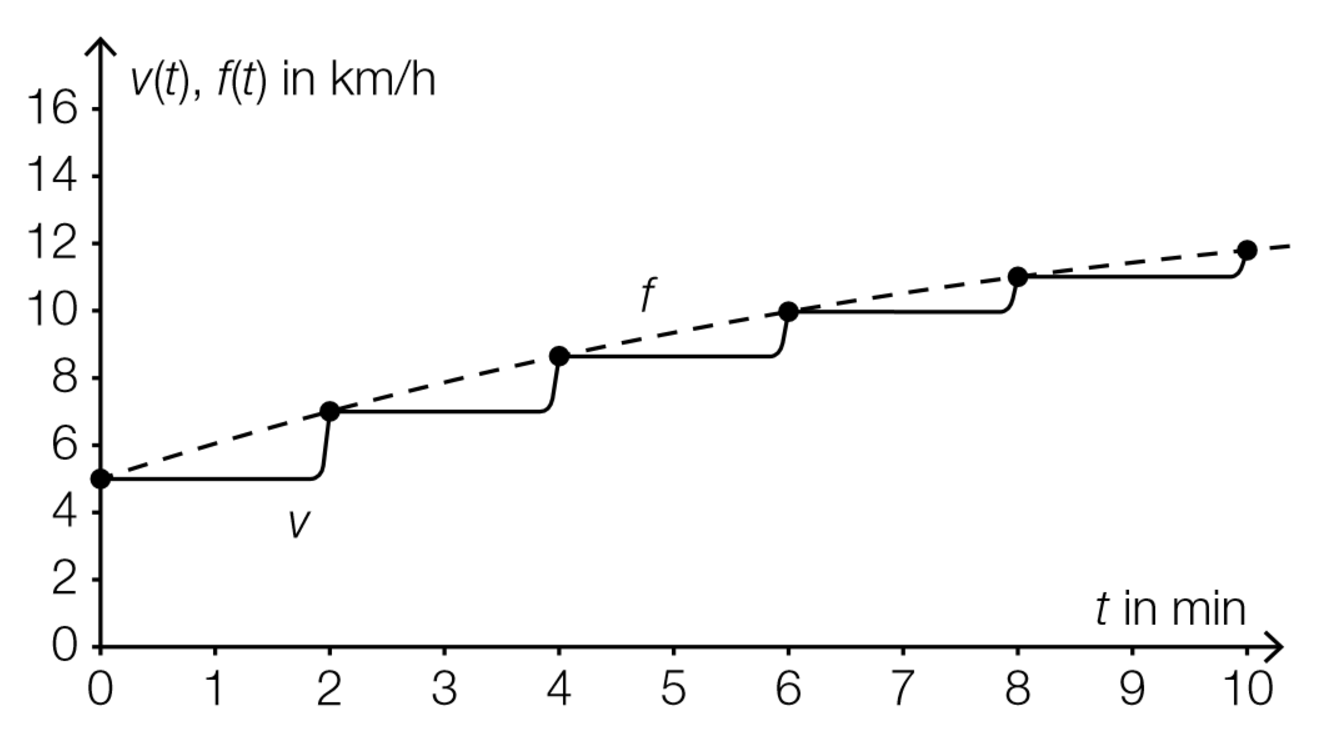
\includegraphics{../Bilder/Bild76-1.eps}}
\end{center}

\subsection{Aufgabenstellung:}
\begin{enumerate}
	\item Gib einen Ausdruck an, mit dem das arithmetische Mittel der Laufbandgeschwindigkeiten w�hrend des 30-min�tigen Trainingsprogramms berechnet werden kann, und ermittle diesen Wert!\leer
	
	Begr�nde, warum das arithmetische Mittel der Laufbandgeschwindigkeiten der mittleren Geschwindigkeit $\bar{v}$ w�hrend des 30-min�tigen Trainingsprogramms entspricht!
	
	Berechne unter Verwendung der mittleren Geschwindigkeit $\bar{v}$ die w�hrend des 30-min�tigen Trainingsprogramms bew�ltigte Strecke!
	
	\item Gib die minimale und die maximale Geschwindigkeit des Laufbands w�hrend des 30-min�tigen Trainingsprogramms an!\leer
	
	$v_\text{min}=$ \rule{5cm}{0.3pt}\,km/h\leer
	
	$v_\text{max}=$ \rule{5cm}{0.3pt}\,km/h\leer
	
	Begr�nde, warum zu den Zeitpunkten $t_{\text{min}}$ und $t_{\text{max}}$, zu denen die minimale bzw. die maximale Geschwindigkeit des Laufbands in dem 30-minptigen Trainingsprogramm erreicht wird, $f'(t_{\text{min}})\neq 0$ und $f'(t_\text{max})\neq 0$ gilt!\leer
	
	\item Gib den Wert von $v'(1)$ an und interpretiere diesen Wert (mit Angabe der Einheit) im gegebenen Kontext!\leer
	
	$v'(1)=$ \rule{5cm}{0.3pt}\leer
	
	Beschreibe anhand des Graphen in der Einleitung, wie der Graph der Ableitungsfunktion $v'$ im Intervall $[0;30]$ verlaufen m�sste!\leer
	
	\item Die in den ersten zehn Trainingsminuten zur�ckgelegte Wegl�nge kann n�herungsweise mit dem Integral $\frac{1}{60}\cdot\int^{10}_0{f(t)}$d$t$ berechnet werden.
	
	Berechne diesen N�herungswert und erl�uter die Bedeutung des Faktors $\frac{1}{60}$!\leer
	
	Gib die absolute Abweichung des berechneten N�herungswertes von der tats�chlich zur�ckgelegten Wegl�nge w�hrend der ersten zehn Minuten in Metern an!	\leer
	
	\item Unter bestimmten Voraussetzungen ist der Energiebedarf einer Person bei einem Lauftraining direkt proportional zur Masse der Person (in kg) und zur zur�ckgelegten Wegl�nge (in km).

Die nachstehende Tabelle zeigt den Energiebedarf (in kcal) einer 80\,kg schweren Person bei einem Lauftraining in Abh�ngigkeit von der Dauer $t$ des Trainings. Die Person l�uft mit einer konstanten Geschwindigkeit von 10\,km/h.

\begin{center}
	\begin{tabular}{|l|l|l|l|l|}\cline{2-5}
	\multicolumn{1}{c|}{}&$t=15$\,min&$t=30$\,min&$t=45$\,min&$t=60$\,min\\ \hline
	Energiebedarf in kcal&194&388&582&776\\ \hline	
	\end{tabular}
\end{center}

Zeige anhand der Tabellenwerte die direkte Proportionalit�t des Energiebedarfs zur zur�ckgelegten Wegstrecke und berechne den Proportionalit�tsfaktor $k$!

Beim Lauftraining wird die Geschwindigkeit h�ufig als "`Tempo"' in min/km umschrieben. Berechne f�r die unten angef�hrten Geschwindigkeiten unter Verwendung des Proportionalit�tsfaktors $k$ f�r eine 90\,kg schwere Person jeweils das Tempo und den Energiebedarf (in kcal) f�r die angegebene Zeitdauer!

\begin{center}
	\begin{tabular}{|p{3cm}|p{3cm}|p{3cm}|p{3cm}|}\hline
	\multirow{2}{2cm}{Geschwindigkeit in km/h}&\multirow{2}{2cm}{Tempo in min/km}&\multirow{2}{2cm}{Energiebedarf in 15\,min}&\multirow{2}{2cm}{Energiebedarf in 30\,min}\\
	&&&\\ \hline \hline
	\multicolumn{1}{|c|}{7,5}&\multicolumn{1}{c|}{8}&&\\ \hline
	\multicolumn{1}{|c|}{10}&&&\\ \hline
	\multicolumn{1}{|c|}{12}&&&\\ \hline	
	\end{tabular}
\end{center}
\end{enumerate}

\antwort{
\begin{enumerate}
	\item \subsection{L�sungserwartung:} 

$\bar{v}=\frac{1}{15}\cdot(f(0)+f(2)+f(4)+...+f(28)\approx 11,57$

Das arithmetische Mittel der Laufbahngeschwindigkeiten betr�gt 11,57\,km/h\leer

Das Arithmetische Mittel entspricht der mittleren Geschwindigkeit w�hrend des 30-min�tigen Trainingsprogramms, weil die Geschwindigkeiten $v(0),...,v(28)$ in gleich langen Zeitintervallen (2\,min) jeweils konstant sind.\leer

zur�ckgelegte Wegl�nge: $0,5\,\text{h}\cdot 11,57\,\text{km/h}=5,785$\,km

	\item \subsection{L�sungserwartung:}
	
	$v_\text{min}=5$\,km/h
	
	$v_\text{max}=14,16$\,km/h\leer
	
	$t_\text{min}$ und $t_\text{max}$ sind keine lokalen Extremstellen der Funktion $f$, weshalb die 1. Ableitung von $f$ an diesen Stellen nicht null ist.

\item \subsection{L�sungserwartung:}
	
$v'(1)=0$

M�gliche Interpretationen:

Die Beschleunigung (momentane Geschwindigkeits�nderung) des Laufbands nach 1 Minute betr�gt 0\,m/s$�$.

oder:

Das Laufband (die L�uferin/der L�ufer) bewegt sich w�hrend der ersten 2 Minuten mit konstanter Geschwindigkeit, d.h., seine Beschleunigung ist zum Zeitpunkt $t=1$\,min gleich null.\leer

Der Graph von $v'$ w�rde auf der 1. Achse verlaufen und nur zu den Zeitpunkten der Geschwindigkeits�nderungen $(t=2, t=4, t=6,...)$ sehr hohe Werte annehmen.

\item \subsection{L�sungserwartung:}
	
$\frac{1}{60}\cdot\int^{10}_0{f(t)}$d$t\approx 1,506$

zur�ckgelegte Wegl�nge: ca. 1,51\,km\leer

M�gliche Begr�ndungen:

Der Faktor $\frac{1}{60}$ ist erforderlich, um die Geschwindigkeiten von km/h in km/min umzurechnen, da die Zeiten (Intervallgrenzen) in Minuten gegeben sind (1\,h=60\,min).

oder:

Der Faktor $\frac{1}{60}$ ist erforderlich, um die pro Stunde zur�ckgelegten Wegstrecken auf die pro Minute zur�ckgelegten Wegstrecken umzurechnen.\leer

F�r die tats�chlich zur�ckgelegte Wegl�nge gilt:

$\frac{2}{60}\cdot(f(0)+f(2)+f(4)+f(6)+f(8))\approx 1,388$\,km

$\Rightarrow$ Der N�herungswert f�r die Wegl�nge weicht um ca. 118\,m vom exakten Wert ab.

\item \subsection{L�sungserwartung:}
	
$194=k\cdot 80\cdot 2,5$

$k=0,97$\leer

Bei der doppelten/dreifachen/vierfachen Laufzeit wird die doppelte/dreifache/vierfache Strecke zur�ckgelegt und auch der Energiebedarf ist doppelt/dreimal/viermal so gro�.

\begin{center}
	\begin{tabular}{|p{3cm}|p{3cm}|p{3cm}|p{3cm}|}\hline
	\multirow{2}{2cm}{Geschwindigkeit in km/h}&\multirow{2}{2cm}{Tempo in min/km}&\multirow{2}{2cm}{Energiebedarf in 15\,min}&\multirow{2}{2cm}{Energiebedarf in 30\,min}\\
	&&&\\ \hline \hline
	\multicolumn{1}{|c|}{7,5}&\multicolumn{1}{c|}{8}&\cellcolor[gray]{0.7}163,7&\cellcolor[gray]{0.7}327,4\\ \hline
	\multicolumn{1}{|c|}{10}&\cellcolor[gray]{0.7}6&\cellcolor[gray]{0.7}218,25&\cellcolor[gray]{0.7}436,5\\ \hline
	\multicolumn{1}{|c|}{12}&\cellcolor[gray]{0.7}5&\cellcolor[gray]{0.7}261,9&\cellcolor[gray]{0.7}523,8\\ \hline	
	\end{tabular}
\end{center}

\end{enumerate}}
		\end{langesbeispiel}%
\hrule  \leer

\section{K1 - QW.bqw - 78 - dsadadad - MC - dadsa}

\begin{langesbeispiel}\item[1] %PUNKTE DER AUFGABE
dsada

\antwort{Themen: QW.bqw (1.)}
\end{langesbeispiel}%
\hrule  \leer

\section{83 - MAT - WS 4.1, AN 1.2, AN 1.3, WS 1.3, WS 1.2 - Wachstumskurve von Kindern - Matura NT 1 16/17}

\begin{langesbeispiel} \item[6] %PUNKTE DES BEISPIELS

Um die Entwicklung der K�rperh�he und der Masse eines Kinder kontrollieren zu k�nnen, sind im Mutter-Kind-Pass die Perzentielenkurven f�r K�rperh�hen (Gr��e) und Masse angegeben (K�rperh�he in cm, Masse in kg). Perzentile teilen die K�rperh�hen und Massen der Kinder in Prozent-Bereiche auf. Liegt ein Wert auf dem 10. Wachstumsperzentil, so sind 10\,\% der Kinder des ausgew�hlten Alters kleiner oder gleich dem angegebenen Wert und 90\,\% gr��er oder gleich dem angegebenen Wert.

Es ist �blich, alle Werte zwischen dem 3. und dem 97. Perzentil als "`normal"' zu bezeichnen. Das folgende Diagramm zeigt die Wachstums- und K�rpermassekurven f�r Buben im Alter von 0 bis 18 Jahren:

\begin{center}
\resizebox{0.8\linewidth}{!}{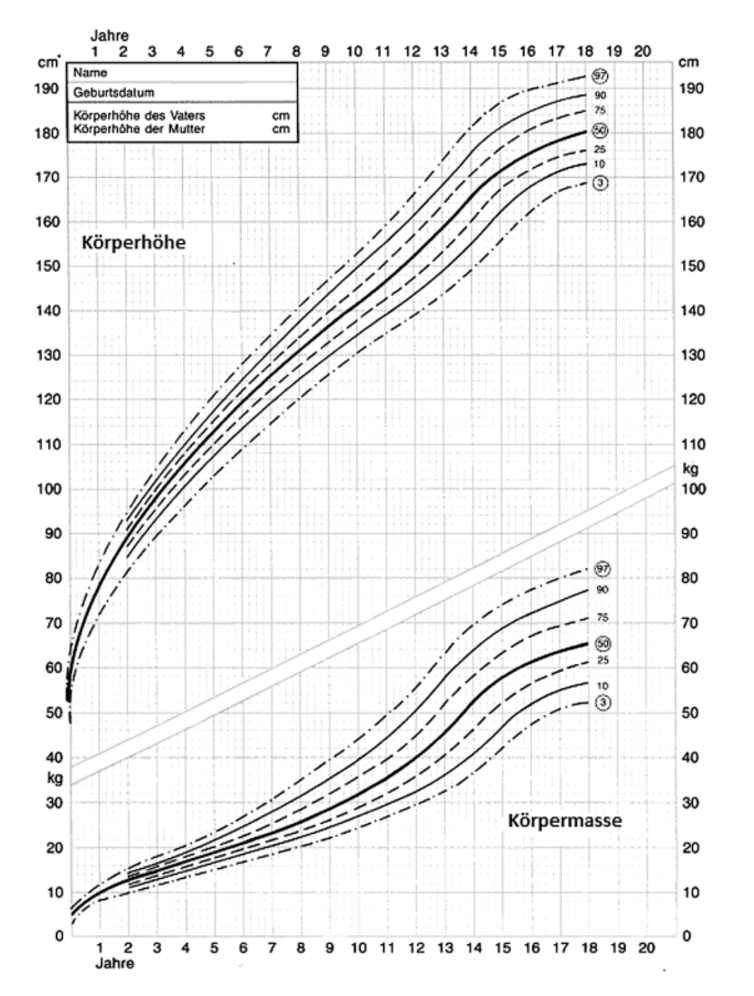
\includegraphics{../Bilder/Bild83-1.eps}}
\end{center}

\subsection{Aufgabenstellung:}
\begin{enumerate}
	\item Ein Schularzt untersucht eine zuf�llige Stichprobe von 8-j�hrigen Buben aus seinem Schulbezirk und erhebt unter anderem deren K�rpermassen (in kg). Anhand der Ergebnisse dieser Messung erstellt er f�r den Anteil der 8-j�hrigen Buben aus einem Schulbezirk, deren K�rpermasse im "`Normalbereich"' $[20\,\text{kg};35\,\text{kg}]$ liegt, das symmetrische Konfidenzintervall $[0,8535;0,9465]$ mit dem Konfidenzniveau $\gamma=0,95$.\leer
	
	Gib den Unterschied des der Berechnung zugrundeliegenden Stichprobenanteils zum Anteil der 8-j�hrigen Buben mit einer K�rpermasse im "`Normalbereich"' laut Diagramm in Prozentpunkten an!\leer
	
	Berechne die Anzahl der bei dieser Stichprobe gemessenen 8-j�hrigen Buben!\leer
	
	\item Angenommen, f�r ein bestimmtes Kind sind die K�rperh�hen $g(1),g(2),g(3),...$ zum ersten, zweiten, dritten usw. Geburtstag bekannt.
	
	Gib verbal oder als Formel an, wie sich die durchschnittliche Wachstumsgeschwindigkeit dieses Kindes in dem dreij�hrigen Zeitraum zwischen dem 6. und dem 9. Geburtstag bestimmen l�sst.\leer
	
	Betrache das Gr��enwachstum auf dem 50. Perzentil nach dem 8. Lebenjahr. Gib das ungef�hre Alter von Buben an, bei dem deren momentane Wachstumsgeschwindigkeit am gr��ten ist!\leer
	
	\item Gib an, welcher statistischen Kennzahl derjenige Wert entspricht, den man auf dem 50. Perzentil ablesen kann.\leer
	
	Erl�utere, welche Schwierigkeiten auftreten, wenn man aus dem angegebenen Diagramm ein Kastenschaubild (Boxplot) zur Darstellung der K�rperh�hen von 8-j�hrigen Buben erstellen m�chte!
	
	\end{enumerate}

\antwort{
\begin{enumerate}
	\item \subsection{L�sungserwartung:} 

Stichprobenanteil: 0,9

Anteil laut Diagramm: 0,94

Unterschied: 4 Prozentpunkte\leer

M�gliche Berechnung:

$0,9465=0,9+1,96\cdot\sqrt{\dfrac{0,9\cdot (1-0,9)}{n}}\Rightarrow\approx 160$ Buben
\subsection{L�sungsschl�ssel:}
\begin{itemize}
	\item Ein Punkt f�r die richtige L�sung.
	\item Ein Punkt f�r die richtige L�sung.
	
	Toleranzintervall: $[155\text{ Buben};165\text{ Buben}]$
	
	Die Aufgabe ist auch dann als richtig gel�st zu werten, wenn bei korrektem Ansatz das Ergebnis aufgrund eines Rechenfehlers nicht richtig ist.
\end{itemize}

	\item \subsection{L�sungserwartung:}

Die durchschnittliche Wachstumsgeschwindigkeit in diesem Zeitraum entspricht einem Drittel der Gr��enzunahme.

oder:

$\frac{g(9)-g(6)}{3}$\leer

Das ungef�hre Alter von Buben, bei dem deren momentane Wachstumsgeschwindigkeit am gr��ten ist, liegt bei ca. 13 Jahren.

\subsection{L�sungsschl�ssel:}
\begin{itemize}
	\item Ein Punkt f�r eine (sinngem��) korrekte Antwort bzw. eine richtige Formel. �quivalente Formeln sind als richtig zu werten.	
	\item Ein Punkt f�r die richtige L�sung, wobei die Einheit "`Jahre"' nicht angef�hrt sein muss.
	
	Toleranzintervall: $[12\text{ Jahre};14\text{ Jahre}]$
\end{itemize}

\item \subsection{L�sungserwartung:}

Die statistische Kennzahl, die demjenigen Wert entspricht, den man auf dem 50. Perzentil ablesen kann, ist der Median.

Die Schwierigkeiten bestehen darin, dass man zwar das 1. und das 3. Quartil sowie den Median, jedoch weder Minimum noch Maximum ablesen kann (und auch keine Informationen bez�glich Ausrei�ern hat).

\subsection{L�sungsschl�ssel:}
\begin{itemize}
	\item Ein Ausgleichspunkt f�r das Anf�hren der korrekten statistischen Kennzahl.
	\item Ein Punkt f�r eine (sinngem��) korrekte Erl�uterung.
\end{itemize}
\end{enumerate}}
		\end{langesbeispiel}%
\hrule  \leer

\section{86 - MAT - AG 2.1, FA 1.4, FA 2.2, FA 2.4, WS 1.1, WS 1.4 - Human Development Index - Matura 2016/17 2. NT}

\begin{langesbeispiel} \item[0] %PUNKTE DES BEISPIELS
Der Human Development Index ($HDI$) der Vereinten Nationen ist ein Wohlstandsindikator für Länder, der eine Messung des Entwicklungsstandes des jeweiligen Landes ermöglichen sollte.
Der $HDI$ beinhaltet drei dimensionslose Größen (Lebenserwartungsindex ($LEI$), Bildungsindex ($BI$)
und Einkommensindex ($EI$)) und wird mit der Formel $HDI=\sqrt[3]{LEI \cdot BI \cdot EI}$ berechnet.

Dimensionslos bedeutet, dass diese Größen keine Einheiten haben.\leer

Für die Berechnung des Indizes $LEI$ und $EI$ gilt seit 2010:

$LEI=\frac{LE-20}{85-20}$, wobei $LE$ die Lebenserwartung zum Zeitpunkt der Geburt in Jahren beschreibt

$EI=\frac{\ln(B)-\ln(100)}{\ln(75\,000)-\ln(100)}$, wobei $B$ das Bruttonationaleinkommen pro Kopf in US-Dollar (immer zu Jahresbeginn) beschreibt.\leer

Das Entwicklungsprogramm der Vereinten Nationen unterteilt die Länder nach dem Wert des $HDI$ seit 2009 in vier Entwicklungskategorien:


\renewcommand{\arraystretch}{1.5}
\begin{center}
\begin{tabular}{c|c} \hline
\rowcolor{lightgray} Entwicklungskategorie eines Landes & Wert des $HDI$ \\ \hline
$E_1$ & $\leq 0,8$ \\ \hline
$E_2$ & $[0,7; 0,8)$ \\ \hline
$E_3$ & $[0,55; 0,7)$ \\ \hline
$E_4$ & $< 0,55$ \\ \hline
\end{tabular}
\end{center}
\tiny Datenquelle: Deutsche Gesellschaft für die Vereinten
Nationen (Hrsg.): Bericht über die menschliche Entwicklung
2015. Arbeit und menschliche Entwicklung. Berlin:
Berliner Wissenschafts-Verlag 2015, S. 240 \normalsize


Der $HDI$ einer Region in einem bestimmten Jahr ergibt sich aus dem arithmetischen Mittel der $HDI$s der zu dieser Region zählenden Länder. \leer

Die Entwicklung des $HDI$ verschiedener Regionen zwischen 1980 und 2011 ist nachstehend abgebildet.

\begin{center}
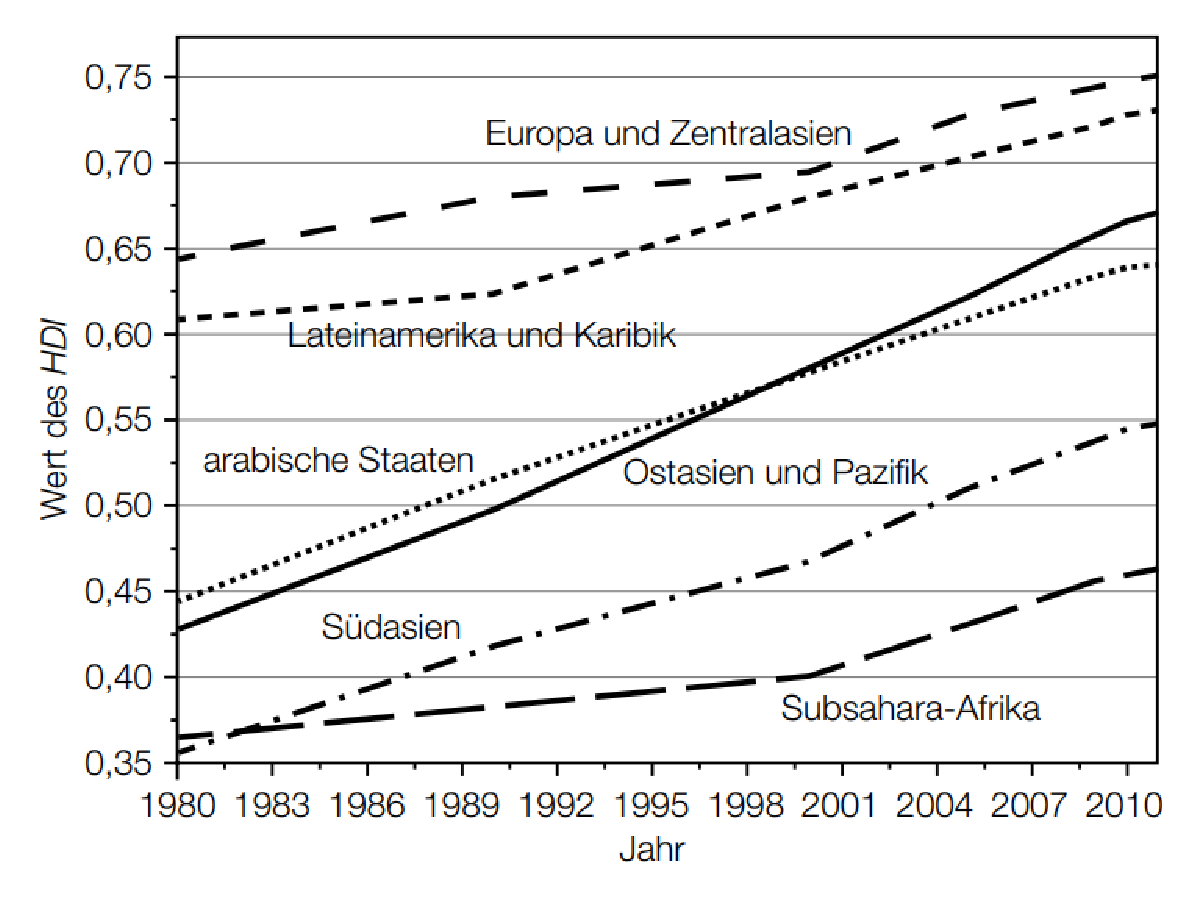
\includegraphics[width=0.7\textwidth]{../Bilder/Bild86-1.eps}
\end{center}
\begin{singlespace}
\tiny Datenquelle: https://de.wikipedia.org/wiki/
Index\_der\_menschlichen\_Entwicklung\#/
media/File:Human-Development-IndexTrends-2011.svg
[08.06.2017]. \normalsize
\end{singlespace}

\subsection{Aufgabenstellung:}

\begin{enumerate}
	\item Für Österreich wurde im Human Development Report für das Jahr 2013 die Lebenserwartung mit $LE = 81,1$ Jahren und der Bildungsindex mit $BI = 0,819$ angegeben. Die nachstehende Abbildung zeigt für die Jahre 2000 bis 2013 (jeweils zu Jahresbeginn) das Bruttonationaleinkommen Österreichs pro Kopf in US-Dollar.
	
\begin{center}
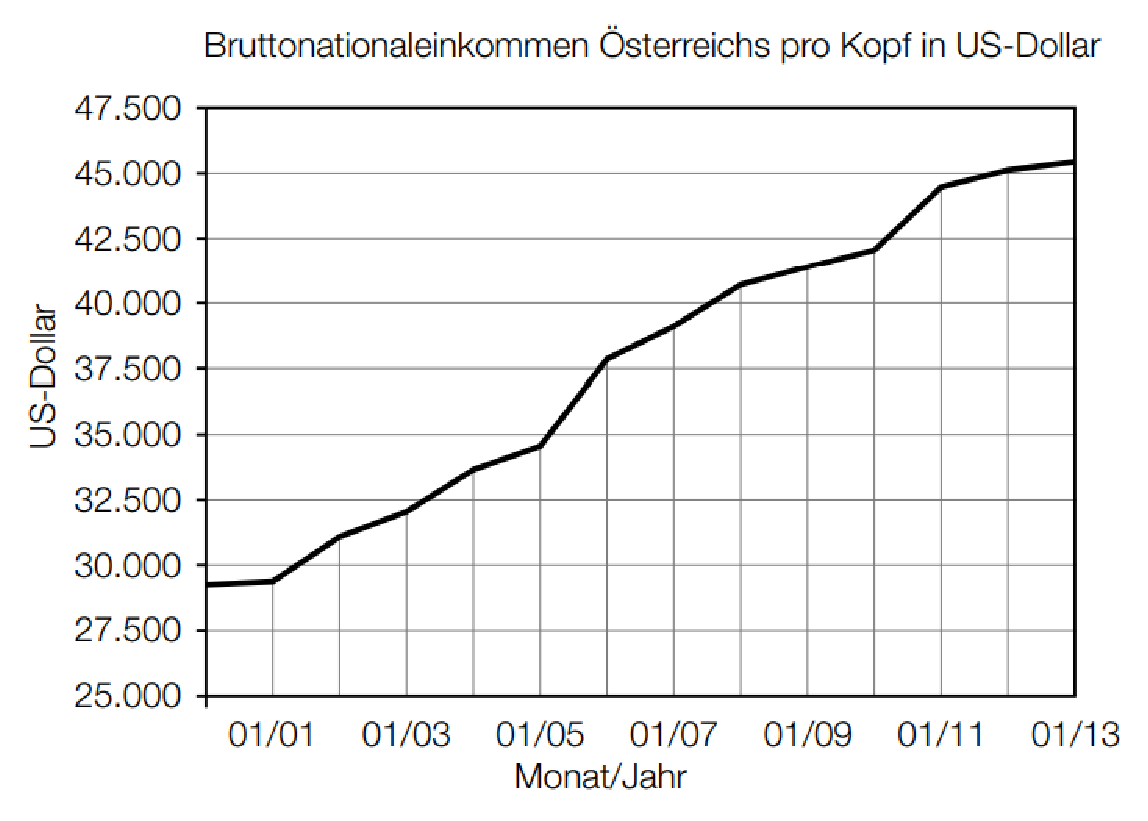
\includegraphics[width=0.6\textwidth]{../Bilder/Bild86-2.eps}
\end{center}	
\tiny Datenquelle: http://www.factfish.com/de/statistik/bruttonationaleinkommen [08.06.2017]. \normalsize

Ermittle für das Jahr 2013 den $HDI$ von Österreich $(=HDI_{2013})$!\leer

Der $HDI$ von Österreich für das Jahr 2013 $(HDI_{2013})$ war um ca. 2,5\,\% größer als der $HDI$ von Österreich für das Jahr 2008 $(HDI_{2008})$. Gib eine Gleichung an, die diesen Zusammenhang beschreibt, und berechne den $HDI_{2008}$!

\item Die jährliche Entwicklung des $HDI$ der Region "`arabische Staaten"' kann im Zeitraum von 1980 bis 2010 näherungsweise durch eine lineare Funktion $H$ mit der Gleichung $H(t) = k \cdot t + d$ mit $k, d \in \mathbb R$ und $t$ in Jahren beschrieben werden, wobei $H(0)$ dem Wert des Jahres 1980 entspricht.\leer

Bestimme die Werte der Parameter $k$ und $d$!\leer

Begründen Sie anhand der entsprechenden Abbildung, in welcher Region/in welchen Regionen die mittlere jährliche Zunahme des $HDI$ im Zeitraum von 1980 bis 2010 am ehesten jener der
Region "`arabische Staaten"' entsprach!

\item \fbox{A} Ermittle aus der entsprechenden Abbildung diejenige Jahreszahl, ab der die Region "`Lateinamerika und Karibik"' die Entwicklungskategorie $E_2$ aufweist!\leer

Gilt ab diesem Zeitpunkt sicher, dass ungefähr die Hälfte der zu dieser Region zählenden Länder
eine Entwicklungskategorie $E_2$ aufweist? Begründe deine Antwort!	
\end{enumerate}

\antwort{
\begin{enumerate}
	\item \subsubsection{Lösungserwartung:}

$LEI=\dfrac{81,1-20}{85-20}=0,94$

$EI\approx \dfrac{\ln(45\,400)-\ln(100)}{\ln(75\,000)-\ln(100)}\approx 0,924$

$HDI_{2013}=\sqrt[3]{0,94\cdot 0,819 \cdot 0,924} \approx 0,893$

$HDI_{2013}=HDI_{2008}\cdot 1,025$

$HDI_{2008}\approx 0,871$

\subsubsection{Lösungsschlüssel}

- Ein Punkt für die richtige Lösung.
Toleranzintervall: $[0,88; 0,91]$
Die Aufgabe ist auch dann als richtig gelöst zu werten, wenn bei korrektem Ansatz das Ergebnis
aufgrund eines Rechenfehlers nicht richtig ist.
- Ein Punkt für eine korrekte Gleichung und die richtige Lösung. Äquivalente Gleichungen sind
als richtig zu werten.
Toleranzintervall: $[0,85; 0,89]$

\item \subsubsection{Lösungserwartung:}

$k=\dfrac{0,64-0,44}{30}=0,006\dot{6}$

$d=0,44$

In der Region "`Südasien"' entsprach die mittlere jährliche Zunahme des HDI im Zeitraum 1980 bis 2010 am ehesten jener der Region "`arabische Staaten"'.

Mögliche Begründung:\\
Die Sekanten durch die Punkte $(1980|0,44)$ und $(2010|0,64)$ sowie $(1980|0,36)$ und $(2010|0,54)$ verlaufen annähernd parallel zueinander. 

\subsubsection{Lösungsschlüssel:}

- Ein Punkt für die Angabe der beiden korrekten Werte.
Toleranzintervall für $k$: $[0,005; 0,01]$
Toleranzintervall für $d$: $[0,43; 0,45]$
- Ein Punkt für die Angabe der Region "`Südasien"' und für eine (sinngemäß) korrekte Begründung.

\item \subsubsection{Lösungserwartung:}

Ab dem Jahr 2004 weist die Region "`Lateinamerika und Karibik"' die Entwicklungskategorie $E_2$
auf.\leer

Nein, es gilt nicht als sicher, dass ab diesem Zeitpunkt ungefähr die Hälfte der zu dieser Region
zählenden Länder die Entwicklungskategorie $E_2$ aufweist.


Mögliche Begründung:
Wenn eine sehr kleine Anzahl an Ländern mit sehr hohen HDI-Werten einer großen Anzahl an
Ländern mit niedrigen $HDI$-Werten $(< 0,7)$ gegenübersteht, kann dennoch das arithmetische
Mittel der $HDI$s größer als $0,7$ sein, ohne dass ungefähr die Hälfte der zu dieser Region zählenden
Länder die Entwicklungskategorie $E_2$ aufweist.

\subsubsection{Lösungsschlüssel:}

- Ein Ausgleichspunkt für die richtige Lösung.
Toleranzintervall: $[2003; 2005]$
- Ein Punkt für eine richtige Antwort und eine korrekte Begründung. Andere korrekte Begründungen
(z.B. anhand sinnvoller Zahlenbeispiele oder mit der Feststellung, dass das arithmetische
Mittel nicht notwendigerweise der Median sein muss) sind ebenfalls als richtig zu
werten.

\end{enumerate}
}

		
\end{langesbeispiel}%
\hrule  \leer

\section{87 - MAT - AN 3.2, AN 3.2, AN 4.3, AN 4.2, WS 3.2 - Dichtefunktion und Verteilungsfunktion - Matura 2016/17 2. NT}

\begin{langesbeispiel} \item[3] %PUNKTE DES BEISPIELS
						Es sei $X$ eine Zufallsvariable, f�r die sich die Wahrscheinlichkeit, dass $X$ in einem Intervall $I$ liegt, mithilfe einer sogenannten Dichtefunktion $f$ folgenderma�en ermitteln l�sst:
						
						$P(a\leq X\leq b)=\displaystyle\int^b_a f(x)$d$x$ f�r alle $a,b\in I$ mit $a\leq b$
						
						In diesem Fall gilt f�r die Verteilungsfunktion $F:F(x)=P(X\leq x)$ f�r alle $x\in\mathbb{R}$, d.h. insbesondere $F(b)-F(a)=P(a\leq X\leq b)$ f�r $a,b\in I$ und $a\leq b$.
						
						Die nachstehende Grafik zeigt den Graphen einer Dichtefunktion $f$ mit $f(x)=k\cdot\sin(x)$ f�r $x\in[0;c]$, wobei $k\in\mathbb{R}, k>0$ und $f(c)=0$ gilt. F�r $x\neq[0;c]$ gilt: $f(x)=0$.
						
						\begin{center}
							\resizebox{0.8\linewidth}{!}{\psset{xunit=4.0cm,yunit=4.0cm,algebraic=true,dimen=middle,dotstyle=o,dotsize=5pt 0,linewidth=1.6pt,arrowsize=3pt 2,arrowinset=0.25}
\begin{pspicture*}(-0.1490384615384615,-0.1384157660521301)(3.2980769230769234,1.2816274634456448)
\psaxes[labelFontSize=\scriptstyle,xAxis=true,yAxis=true,labels=y,Dx=0.2,Dy=1.,yticksize=-2pt 0,xticksize=0]{->}(0,0)(0.,0.)(3.2980769230769234,1.2816274634456448)[x,140] [f(x),-40]
\psplot[linewidth=2.pt,plotpoints=200]{0}{3.14}{0.5*SIN(x)}
\antwort{\psplot[linewidth=2.pt,plotpoints=200]{0}{3.14}{-1.0/2.0*COS(x)+0.5}}
\rput[tl](3.1153846153846154,-0.03075905912269592){c}
\rput[tl](2.331730769230769,0.5075244755244751){$f$}
\antwort{\rput[tl](2.394230769230769,1.0406815003178636){$F$}}
\end{pspicture*}}
						\end{center}

				\subsection{Aufgabenstellung:}
\begin{enumerate}
	\item Gib f�r die gegebenen Dichtefunktion $f$ den Funktionswert $F(0)$ der zugeh�rigen Verteilungsfunktion $F$ an und begr�nde, warum $F(c)=1$ ist!\leer
	
	$F(0)=$\,\antwort[\rule{3cm}{0.3pt}]{0}
	
	Skizziere in der oben stehenden Grafik den Graphen der zugeh�rigen Verteilungsfunktion $F$ und beschreibe das Kr�mmungsverhalten von $F$ im Intervall $[0;c]$!
	
	\item Gib an, durch welche Eigenschaft von $f$ der Wert des Parameters $k$ festgelegt ist, und berechne den Wert von $k$!
	
	Gib einen Term der zugeh�rigen Verteilungsfunktion $F$ im Intervall $[0;c]$ an!\leer
	
	$F(x)=$\,\antwort[\rule{3cm}{0.3pt}]{$-0,5\cdot\cos(x)+0,5$}
	
	\item F�r ein Ereignis $E$ gilt: $P(E)=1-P(X\leq c-a)$ f�r ein beliebiges $a\in[0;c]$.
	
	\fbox{A} Beschreibe dieses Ereignis $E$ verbal!
	
	Stelle f�r $a\leq\frac{c}{2}$ die Wahrscheinlichkeit $P(a\leq X\leq c-a)$ in nachstehender Grafik als Fl�che dar und begr�nde den Zusammenhang \\ \mbox{$P(a\leq X\leq c-a)=1-2\cdot P(X\leq a)$} anhand dieser Darstellung!
	
	\begin{center}
		\resizebox{0.8\linewidth}{!}{\psset{xunit=4.0cm,yunit=4.0cm,algebraic=true,dimen=middle,dotstyle=o,dotsize=5pt 0,linewidth=1.6pt,arrowsize=3pt 2,arrowinset=0.25}
\begin{pspicture*}(-0.1490384615384615,-0.1384157660521301)(3.2980769230769234,1.2816274634456448)
\psaxes[labelFontSize=\scriptstyle,xAxis=true,yAxis=true,labels=y,Dx=0.2,Dy=1.,yticksize=-2pt 0,xticksize=0]{->}(0,0)(0.,0.)(3.2980769230769234,1.2816274634456448)[x,140] [f(x),-40]
\psplot[linewidth=2.pt,plotpoints=200]{0}{3.14}{0.5*SIN(x)}
\rput[tl](3.1153846153846154,-0.0307){c}
\rput[tl](2.331730769230769,0.5075244755244751){$f$}
\antwort{\pscustom[linewidth=0.8pt,fillcolor=black,fillstyle=solid,opacity=0.1]{\psplot{1.0471975511965976}{2.0943951023931953}{0.5*SIN(x)}\lineto(2.0943951023931953,0)\lineto(1.0471975511965976,0)\closepath}
\rput[tl](1.0144230769230769,-0.0307){$a$}
\rput[tl](2.0,-0.0307){$c-a$}}
\end{pspicture*}}
	\end{center}
	
						\end{enumerate}\leer
				
\antwort{
\begin{enumerate}
	\item \subsection{L�sungserwartung:}
	$F(c)=1$ bzw. $P(X\leq c)=1$, d.h., die Wahrscheinlichkeit, dass $X$ einen Wert kleiner gleich $c$ annimmt, betr�gt 100\,\%, da $f(x)=0$ f�r $x>c$.
	
	Skizze: siehe oben.
	
	Bis zum lokalen Maximum von $f$ ist die Funktion $F$ linksgekr�mmt, danach ist die Funktion $F$ rechtsgekr�mmt.
	
	\subsection{L�sungsschl�ssel:}
	
	- Ein Punkt f�r die richtige L�sung und eine (sinngem��) korrekte Begr�ndung.
	
	- Ein Punkt f�r eine korrekte Skizze und eine (sinngem��) korrekte Beschreibung des Kr�mmungsverhaltens der Funktion $F$. Die Skizze ist als korrekt zu betrachten, wenn das korrekte Kr�mmungsverhalten des Graphen von $F$ in der Skizze klar erkennbar ist und die Wendestelle von $F$ dabei bei $x=\frac{c}{2}$ liegt. F�r $x>c$ muss der Graph von $F$, sofern er in diesem Bereich skizziert ist, waagrecht verlaufen.
	
	\item \subsection{L�sungserwartung:}
	
	Der Wert von $k$ ist durch die Eigenschaft $F(c)=1$ festgelegt, d.h., der Inhalt der vom Graphen von $f$ und der $x$-Achse im Intervall $[0;c]$ eingeschlossenen Fl�che muss 1 sein. Da die rechte Nullstelle bei $x=\pi$ liegt und somit $c=\pi$ ist, muss gelten:
	
	$\displaystyle\int^\pi_0\,k\cdot\sin(x)$d$x=1 \Rightarrow k=0,5$
	
	M�gliche Vorgehensweise:
	
	$F(x)=-0,5\cdot\cos(x)+C$
	
	$F(0)=0 \Rightarrow C=0,5$
	
	$F(x)=-0,5\cdot\cos(x)+0,5$
	
	\subsection{L�sungsschl�ssel:}
	
	- Ein Punkt f�r eine (sinngem��) korrekte Angabe, welche Eigenschaft von $f$ den Wert von $k$ festlegt, und f�r die richtige L�sung.
	
	- Ein Punkt f�r einen korrekten Term. �quivalente Terme sind als richtig zu werten.
	
	\item \subsection{L�sungserwartung:}
	
	Das Ereignis $E$ beschreibt, dass die Zufallsvariable $X$ einen Wert annimmt, der gr��er (oder gleich) $c-a$ ist.
	
	Grafik siehe oben
	
	M�gliche Begr�ndung:
	
	Wegen der Symmetrie der Dichtefunktion gilt: $P(X\leq a)=P(x\geq c-a)$.
	
	Aus $F(c)=1$ folgt: $P(a\leq X\leq c-a)=1-P(X\leq a)-P(X\geq c-a)=1-2\cdot P(X\leq a)$.
	
	\subsection{L�sungsschl�ssel:}
	
	- Ein Ausgleichspunkt f�r eine (sinngem��) korrekte Beschreibung.
	
	- Ein Punkt f�r eine korrekte Darstellung der Wahrscheinlichkeit als Fl�che, wobei die beiden Grenzen symmetrisch zur Stelle des Maximums der Funktion $f$ liegen m�ssen, und eine korrekte Begr�ndung. Andere korrekte Begr�ndungen sind ebenfalls als richtig zu werten.
		\end{enumerate}}		
	
		\end{langesbeispiel}%
\hrule  \leer

\end{document}